% This is the Reed College LaTeX thesis template. Most of the work
% for the document class was done by Sam Noble (SN), as well as this
% template. Later comments etc. by Ben Salzberg (BTS). Additional
% restructuring and APA support by Jess Youngberg (JY).
% Your comments and suggestions are more than welcome; please email
% them to cus@reed.edu
%
% See http://web.reed.edu/cis/help/latex.html for help. There are a
% great bunch of help pages there, with notes on
% getting started, bibtex, etc. Go there and read it if you're not
% already familiar with LaTeX.
%
% Any line that starts with a percent symbol is a comment.
% They won't show up in the document, and are useful for notes
% to yourself and explaining commands.
% Commenting also removes a line from the document;
% very handy for troubleshooting problems. -BTS

% As far as I know, this follows the requirements laid out in
% the 2002-2003 Senior Handbook. Ask a librarian to check the
% document before binding. -SN

%%
%% Preamble
%%
% \documentclass{<something>} must begin each LaTeX document

\documentclass[oneside]{report}
\usepackage{Suthesis-2e}
% Packages are extensions to the basic LaTeX functions. Whatever you
% want to typeset, there is probably a package out there for it.
% Chemistry (chemtex), screenplays, you name it.
% Check out CTAN to see: http://www.ctan.org/
%%
\usepackage{graphicx,latexsym}
\usepackage{amsmath}
\usepackage{amssymb,amsthm}
\usepackage{longtable,booktabs,setspace}
\usepackage{chemarr} %% Useful for one reaction arrow, useless if you're not a chem major
\usepackage[hyphens]{url}
% Added by CII
\usepackage[draft]{hyperref}
\usepackage{lmodern}
\usepackage{float}
\floatplacement{figure}{H}
% End of CII addition
\usepackage{rotating}

% Next line commented out by CII
%%% \usepackage{natbib}
% Comment out the natbib line above and uncomment the following two lines to use the new
% biblatex-chicago style, for Chicago A. Also make some changes at the end where the
% bibliography is included.
%\usepackage{biblatex-chicago}
%\bibliography{thesis}


% Added by CII (Thanks, Hadley!)
% Use ref for internal links
\renewcommand{\hyperref}[2][???]{\autoref{#1}}
\def\chapterautorefname{Chapter}
\def\sectionautorefname{Section}
\def\subsectionautorefname{Subsection}
% End of CII addition

% Added by CII
\usepackage{caption}
\captionsetup{width=5in}
% End of CII addition

% \usepackage{times} % other fonts are available like times, bookman, charter, palatino

% Syntax highlighting #22

% Added by KM to include latex packages
	\usepackage{array}
	\usepackage{float}
	\usepackage{tabularx}
	\usepackage{longtable}
	\usepackage{afterpage}
	\usepackage{threeparttable}

% To pass between YAML and LaTeX the dollar signs are added by 
\setstretch{1.6}
\begin{document}
\title{Polite language reflects competing social goals}
\author{Erica J. Yoon}
% The month and year that you submit your FINAL draft TO THE LIBRARY (May or December)
\date{May 2019}
\dept{Psychology}
\principaladviser{Michael C. Frank}
\firstreader{Ellen Markman}
\secondreader{Noah Goodman}
  \thirdreader{Hyowon Gweon} %if needed

% if you're writing a thesis in an interdisciplinary major,
% uncomment the line below and change the text as appropriate.
% check the Senior Handbook if unsure.
%\thedivisionof{The Established Interdisciplinary Committee for}
% if you want the approval page to say "Approved for the Committee",
% uncomment the next line
%\approvedforthe{Committee}

% Added by CII
%%% Copied from knitr
%% maxwidth is the original width if it's less than linewidth
%% otherwise use linewidth (to make sure the graphics do not exceed the margin)
\makeatletter
\def\maxwidth{ %
  \ifdim\Gin@nat@width>\linewidth
    \linewidth
  \else
    \Gin@nat@width
  \fi
}
\makeatother

\renewcommand{\contentsname}{Contents}
% End of CII addition

\setlength{\parskip}{0pt}

% Added by CII

\providecommand{\tightlist}{%
  \setlength{\itemsep}{0pt}\setlength{\parskip}{0pt}}




\beforepreface
\prefacesection{Abstract}
We use polite speech on a daily basis. From ``thanks'' and ``please'' to
``your dress is cute'' to ``these cookies could use a bit of salt,''
people often produce polite utterances that are indirect or even false
to some degree. Why do people speak politely? This thesis proposes a
goal-based account of polite speech, that polite speech arises from a
set of competing social goals: the speaker's desire to transfer
information in the most truthful and informative manner possible
(``informational goal''), and to abide by social norms and expectations
and/or maintain the interactants' \emph{face} or public self-image
(``pro-social goal'') and/or present herself as a particular kind of
individual (e.g., kind, helpful person; ``self-presentational goal'').
In Chapter 1, I provide an overview of this integrative theoretical
framework that aims to unify previous theoretical accounts of polite
speech and explain existing empirical studies on understanding and
production of polite speech in adults and children. In Chapter 2, I
provide a computational model that formalizes the notion of goals as
utilities that speakers try to maximize through language use, and show
that this model successfully captures adults' predictions and judgments
for polite lies and indirect speech. Then I present two sets of
empirical studies looking at the development of polite language
understanding: 2- to 4-year-old children's judgments for polite requests
(Chapter 3) and 5- to 8-year-old children's judgments for polite lies
versus blunt truths (Chapter 4). Overall, the work presented in this
thesis reveals how adults and children's understanding of polite speech
reflects their understanding of speaker goals to be informative and
social.

\prefacesection{Dedication}
FIXME
%\prefacesection{}
%This thesis is dedicated to 
\prefacesection{Acknowledgments}
FIXME

\afterpreface


\chapter*{Introduction}\label{intro}
\addcontentsline{toc}{chapter}{Introduction}

We use and hear polite speech on a daily basis, ranging from simple
words of apology (``sorry'') or gratitude (``thanks'') to compliments
(``I love your dress!'') and requests (``Can you please open the
window?''). Adults and even young children spontaneously produce
requests in polite forms (Axia \& Baroni, 1985; H. H. Clark \& Schunk,
1980). Speakers exhibit politeness strategies even while arguing,
preventing unnecessary offense to their interactants (Holtgraves, 1997).
Listeners even attribute ambiguous speech to a polite desire to hide a
truth that could hurt another's self-image (e.g., Bonnefon, Feeney, \&
Villejoubert, 2009). In fact, it is difficult to imagine human speech
that efficiently conveys only the truth. Intuitively, politeness is one
prominent characteristic that differentiates human speech from
stereotyped robotic communication, which may try to follow rules to say
``please'' or ``thank you'' yet still lack genuine politeness.

Although language users use polite speech on a daily basis, explaining
why we use polite speech or how we understand it is not as
straightforward as it first seems. While very simple polite utterances
can be produced from straightforward rules (e.g., say ``sorry'' when you
did something bad to someone), When speakers want to tell the listener
to ``close the window,'' they often use a more roundabout way and say
``can you please close the window?'' When people see that their
interactant is wearing a new outfit that they think is hideous, they
might still say ``Your dress looks gorgeous!'' As such, polite
utterances often seem to misrepresent their intended message or conceal
the truth, which shows that polite speech violates a critical principle
of cooperative communication: exchanging information efficiently and
accurately (Grice, 1975).

If politeness only gets in the way of effective information transfer,
why be polite? Clearly, there are social concerns, and most linguistic
theories assume utterance choices are motivated by these concerns,
couched as either polite maxims (G. Leech, 1983), social norms (Ide,
1989), or aspects of a speaker and/or listener's identity, known as
\emph{face} (P. Brown \& Levinson, 1987; Goffman, 1967). All of these
theories use different approaches to explain polite language, and some
are even framed as counterarguments to existing theories (e.g., see
Watts, 2003, and @matsumoto1988 for counterarguments to some issues in
P. Brown \& Levinson (1987)). One possible commonality among these
theories however, is that they all describe ways in which language
communication deviates from certain expected utterances or conversations
due to speakers' social concerns.

In this thesis, my goal is to offer an integrative theoretical framework
that aims to unify these existing theories, and provide empirical
evidence in support of this framework. Specifically, I argue for a
\emph{goal-based} theory of polite speech: that polite utterances arise
from competing social goals that speakers have, such as their desires to
convey information as truthfully and efficiently as possible
(``informational goal''), to make the listeners feel happy and respected
and thereby boost or maintain their face (``prosocial goal''), and to
present speakers themselves in a good light (e.g., that they are kind
and helpful; ``presentational goal''). Speakers then have to consider
the tradeoff between these goals, and think about which goal to
prioritize and how much to do so to determine their utterance.

For example, imagine that Alice and Bob are having a conversation and
Bob asks for Alice's feedback on his cookies that he baked (``How did
you like my cookies?'') and Alice thinks the cookies tasted bad and
salty (Figure~\ref{fig:schematic-overview}, top panel). Alice's
utterance would differ depending on her goals: whether she wants to
prioritize informational goal or telling the truth to Bob; social goal
or making Bob feel happy; or presentational goal or presenting Alice
herself in a good light that she is kind (Predictions of this specific
scenario will be explained in detail in Chapter 2).

The contents of this dissertation will be as follows, as shown in Figure
1: In Chapter 1 (top panel of Figure~\ref{fig:schematic-overview}) I
present an integrative goal-based framework that aims to explain polite
speech based on the idea that it reflects a tradeoff between competing
social goals that speakers have. Then using this framework, I will
explain existing empirical studies on understanding and production of
polite speech in adults and children. Chapters 2-4 describe a set of
computational and empirical studies of children and adult's
understanding of polite language (bottom panels of
Figure~\ref{fig:schematic-overview}) . In Chapter 2, I provide a
computational model that formalizes the notion of goals as utilities
that speakers try to maximize through language use, and show that this
model successfully captures adults' predictions and judgments for polite
lies and indirect speech. Then I present two sets of empirical studies
looking at the development of polite language understanding: Chapter 3
examines 2- to 4-year-old children's judgments for polite requests, and
Chapter 4 looks at 5- to 8-year-old children's judgments for polite lies
versus blunt truths.
\begin{figure}[!t]

{\centering 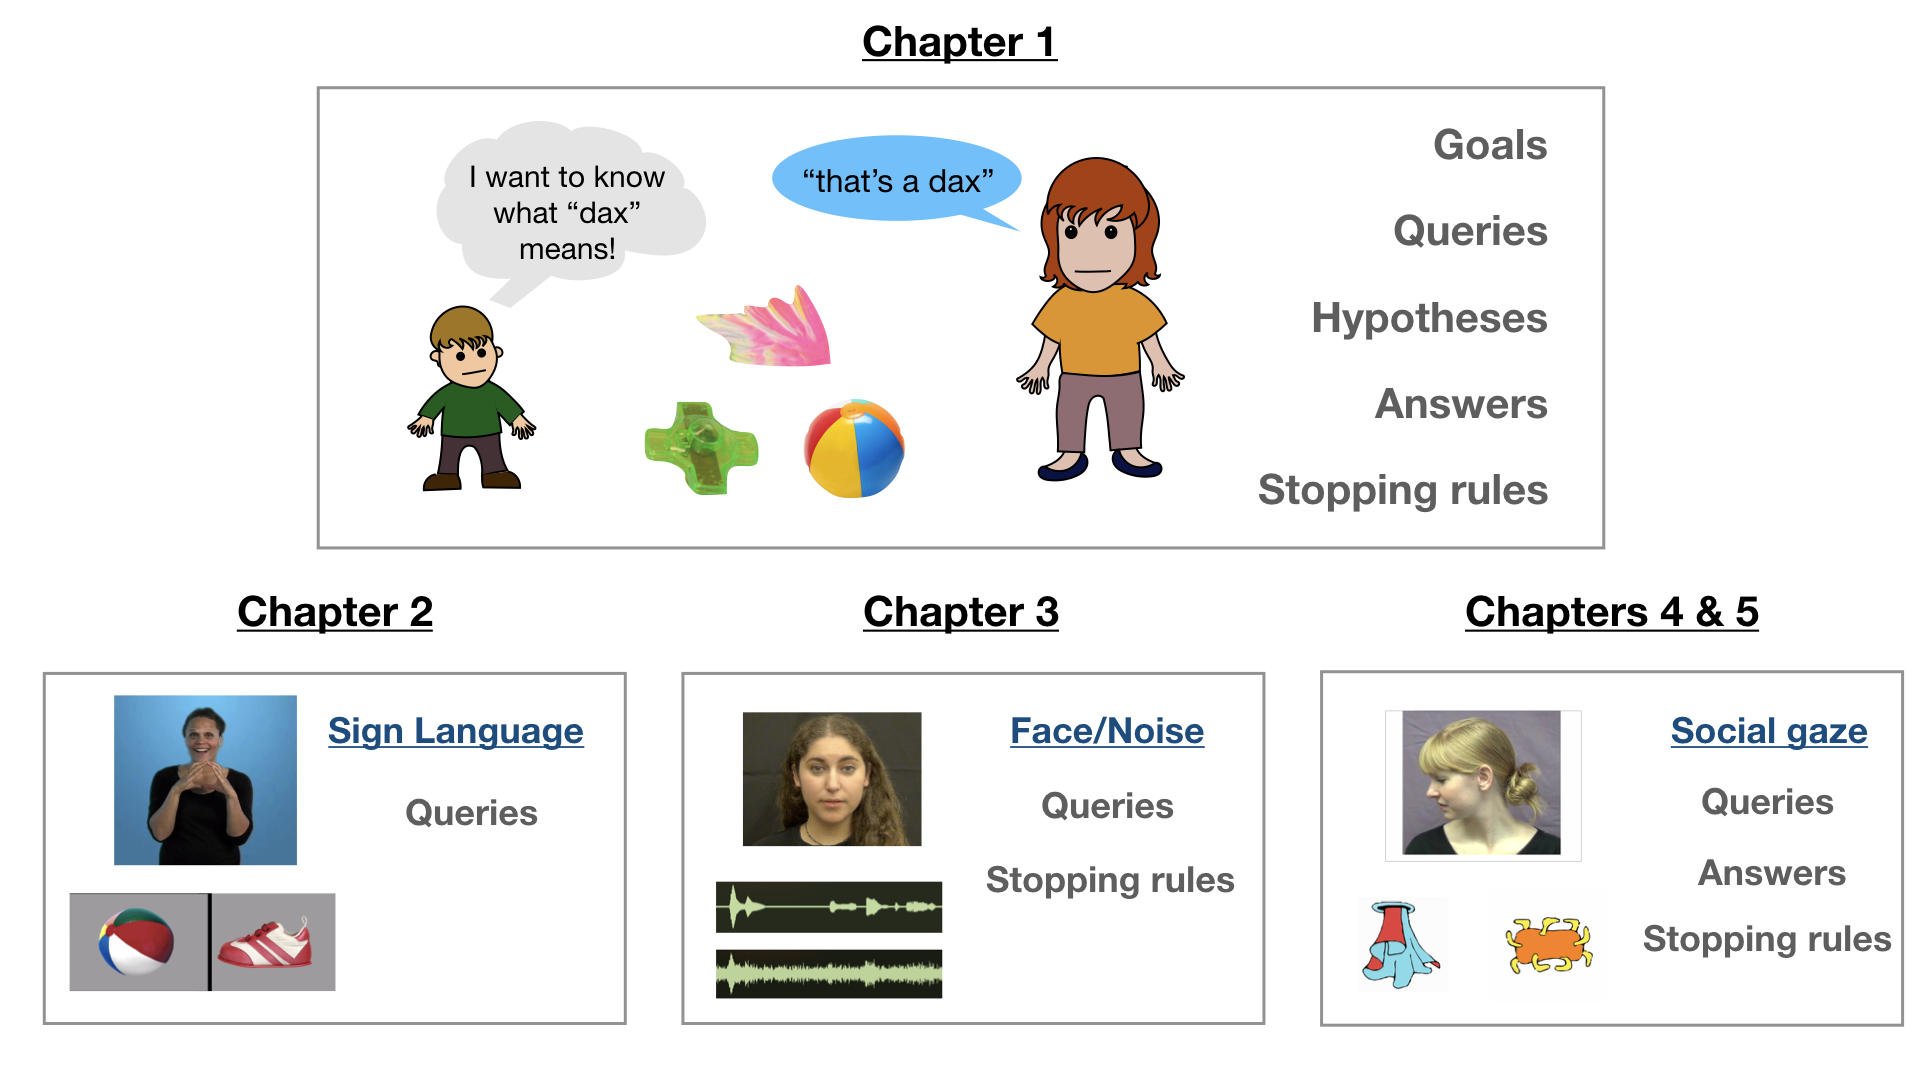
\includegraphics[width=0.9\linewidth]{/Users/ejyoon/Documents/Documents/Research/dissertation/index/chapter_child_rmds/Intro/figs/schematic_overview} 

}

\caption[Schematic overview of the dissertation content.]{The upper panel shows a schematic overview of an integrative framework of polite language understanding based on competing social goals. The lower panels show different studies examining adults' and children's understanding of different component goals (and possible tradeoffs between them) that correspond to each chapter of the dissertation.}\label{fig:schematic-overview}
\end{figure}
\chapter{Children's information seeking within social learning
contexts}\label{childrens-information-seeking-within-social-learning-contexts}

\chaptermark{Information seeking within social contexts}

\section{Introduction}\label{introduction}

Early cognitive development is remarkable. Consider that children,
despite limitations on their processing capabilities and ambiguity in
the input, rapidly acquire new lexical concepts, eventually reaching an
adult vocabulary ranging from 50,000 to 100,000 words (P. Bloom, 2002).
And they accomplish this all while also developing motor skills,
learning social norms, and building causal knowledge. How can we explain
the children's prodigious learning abilities?

Social learning accounts point out that children do not solve these
problems on their own. Instead, they are typically surrounded by
parents, other knowledgeable adults, or older peers -- all of whom are
likely to know more than they do and want to facilitate their learning.
Social learning accounts also emphasize how social contexts can
bootstrap children's learning via several, distinct mechanisms. For
example, work on early language acquisition shows that social partners
provide input that is tuned to children's cognitive abilities (Eaves Jr,
Feldman, Griffiths, \& Shafto, 2016; Fernald \& Kuhl, 1987), that guides
children's attention to important features in the world (Yu \& Ballard,
2007), and increases levels of sustained attention, which results in
better learning outcomes (P. K. Kuhl, 2007; Yu \& Smith, 2016).

Social contexts can also change the inferences that support children's
learning from evidence. Recent work in the fields of concept learning
and causal intervention suggests that the presence of another person
engages a set of psychological reasoning where the learner thinks about
\emph{why} other people performed specific actions. The critical insight
comes from knowing that another person has intentionally selected
examples, which allows children to make stronger inferences that speed
learning (Bonawitz \& Shafto, 2016; Frank, Goodman, \& Tenenbaum, 2009;
Shafto, Goodman, \& Griffiths, 2014). For example, children learn at
different rates after observing the same evidence depending on whether
they thought the actions that generated that evidence were accidental
(less informative) or intentionally selected (more informative).
Moreover, adults and children will make even stronger inferences if they
believe that another person selected their actions with the goal of
helping them to learn (i.e., teaching) (Shafto, Goodman, \& Frank,
2012b).

However, children are not passive recipients of information -- from
people or the world. Instead, they actively select behaviors -- for
example, asking questions or choosing where to allocate visual attention
-- that can change the content, pacing, and sequence of their learning
experience. Recent theories of cognitive development have proposed the
metaphor of the ``child as a scientist'' and characterized early
learning as a process of exploration and hypothesis testing following
principles of the scientific method (Gopnik, Meltzoff, \& Kuhl, 1999; L.
Schulz, 2012). Moreover, empirical work across a variety of domains --
education (Grabinger \& Dunlap, 1995), machine learning (Castro et al.,
2009; Settles, 2012), and cognitive science (D. B. Markant \& Gureckis,
2014) -- has directly compared learning trajectories in self-directed
contexts (active learning) as compared to settings where the learner has
less control (passive learning). The upshot of this work is that active
contexts often lead to faster learning because of enhanced attention and
arousal or because learners select information that is closely linked to
their current goals, uncertainty, and skill (see Gureckis \& Markant
(2012) for a review).

Thus, children are capable of selecting actions to support their
learning, and a large body of work shows that social partners can create
particularly rich contexts for learning. Empirical work within each
framework, however, has often focused on the separate effects of active
or social processes. This approach, however, does not reflect the
ecological context in which language acquisition unfolds. That is,
children acquire their first language from interactions with other
people where they have the opportunity to select actions -- where to
look, where to point, what question to ask -- that influence the content
and pacing of the experience. The mismatch between the existing
empirical work and children's natural learning environments highlights
the need for integration across the active and social theoretical
accounts.

But how can we integrate these two proposals, which often include
definitional issues and a lack of formal foundations? In this chapter, I
present an integrated account of active learning within social contexts,
arguing that it represents an important step for theories of early
cognitive development. To connect the active and social learning
proposals, I use the computational frameworks of Optimal Experiment
Design (Emery \& Nenarokomov, 1998; Lindley, 1956) and Bayesian models
of social reasoning (Goodman \& Frank, 2016). The key insight is that
the presence of another person can modulate the \emph{availability} and
\emph{usefulness} of different actions that the active learner could
select. Specifically, social interactions can shape learners' goals,
hypotheses, actions, answers, and decisions about when to stop gathering
information.

In addition to the theoretical account, this chapter provides concrete
definitions of active and social learning to clarify the behaviors and
phenomena that the account aims to address
(\protect\hyperlink{scope}{Part I}). Then, I briefly review the
framework of Optimal Experiment Design (OED)
(\protect\hyperlink{oed}{Part II}), highlighting how it can be can be
used to formalize human information seeking behaviors. I also discuss
the empirical evidence for OED-like reasoning in both adults' and
children's learning. Finally, I conclude by presenting the integrative
account of how social contexts can shape information seeking
(\protect\hyperlink{active_social}{Part III}). In the final section, I
also highlight a series of new links between the social and active
accounts, which present a way forward for empirical work that sheds
light on how children's active learning operates over fundamentally
social input.

\hypertarget{scope}{\section{Part I: Learning from others and learning
on your own}\label{scope}}

A diverse set of scholars, theories, and empirical work has considered
the contributions of active and social processes to children's learning.
One consequence of this range of approaches is that the terms ``active''
and ``social'' have become associated with a variety of meanings. Thus,
before integrating the two accounts, it is worth defining what I mean by
active learning and social contexts. By providing clear definitions,
this section aims to clarify the behaviors and phenomena that the
integrative account attempts to explain.

\subsection{Social learning}\label{social-learning}

Learning can be social in a variety of ways. First, children could learn
with another person present but without attending to or directly
interacting with them. Research in social psychology shows that the mere
presence of other people can facilitate the performance of simple tasks
and impair the performance of complex tasks (N. B. Cottrell, Wack,
Sekerak, \& Rittle, 1968; Uziel, 2007). Second, children could learn by
looking to others as a guide and observing or imitating their behavior.
Children's capacity for faithful imitation has been argued to be a
critical feature separating human from non-human learning (Call,
Carpenter, \& Tomasello, 2005). Finally, children could both attend to
the person and directly interact with them, entering a communicative
learning context that engages psychological reasoning processes that
alter the course of learning (Frank \& Goodman, 2014; Goodman \& Frank,
2016; Shafto et al., 2012b).

For the integrative account discussed in this chapter, I define a social
context as a learning environment where another agent is present. This
definition includes all of the social learning behaviors -- observation,
imitation, and learning from direct interaction -- mentioned above. This
broad definition highlights the diverse pathways through which social
information could interact with children's active learning. Moreover,
this definition captures the variety of contexts in which children
develop, i.e., in some cultures children experience high amounts of
child-centered interactions while in others they are often expected to
learn through observation of older peers and adults (Rogoff et al.,
1993).

Social learning theories emphasize that children's rapid conceptual
development is facilitated by the uniquely human capacity to transmit
and acquire information from other people. A primary benefit of learning
from others is that children gain access to knowledge that has
accumulated over many generations; information that would be too complex
for any individual to figure out on their own (Boyd, Richerson, \&
Henrich, 2011). In addition to the cumulative effects, social contexts
facilitate in-the-moment learning since more knowledgeable others can
provide input that is most useful for children (Kline, 2015; Shafto et
al., 2012b) and communicate information that is likely to generalize to
other contexts (Csibra \& Gergely, 2009).

There is a large body of empirical work showing the effects of social
input in a variety of domains, including language acquisition, causal
learning, and concept learning. For example, newborn infants prefer to
look at face-like patterns compared to other abstract configurations
(Farroni, Csibra, Simion, \& Johnson, 2002; Johnson, Dziurawiec, Ellis,
\& Morton, 1991), to listen to speech over non-speech (Vouloumanos \&
Werker, 2007), their mother's voice over a stranger's (DeCasper, Fifer,
Oates, \& Sheldon, 1987), and infant-directed speech over adult-directed
speech (Cooper \& Aslin, 1990; Fernald \& Kuhl, 1987; Pegg, Werker, \&
McLeod, 1992). Moreover, these attentional biases lead to differential
learning in the presence of another person. 4-month-olds show better
memory for faces that gazed directly at them (Farroni, Massaccesi,
Menon, \& Johnson, 2007), for an object if an adult gazed at that object
during learning (Cleveland, Schug, \& Striano, 2007; Reid \& Striano,
2005), and perform better at tasks such as segmenting words from
infant-directed speech compared to adult-directed speech (Thiessen,
Hill, \& Saffran, 2005). P. K. Kuhl (2007) refer to these effects as
``social gating'' phenomena since the presence of another person
activates or enhances children's underlying learning mechanisms.

In addition to enhancing attention and memory, social contexts can
facilitate learning by generating useful information tailored to the
child's current developmental stage (Vygotsky, 1987). Empirical work
shows that caregivers alter their communication style when speaking to
children (e.g.,exaggerating prosody, reducing speed), which in turn can
help children learn vowel sounds (Adriaans \& Swingley, 2017; De Boer \&
Kuhl, 2003), segment the speech stream (Fernald \& Mazzie, 1991;
Thiessen et al., 2005), recognize familiar words (Singh, Nestor, Parikh,
\& Yull, 2009) and learn new lexical concepts (Graf Estes \& Hurley,
2013). Additional evidence comes from studies of early vocab development
showing that infants will produce more speech-like sounds when
interacting with caregivers who provide contingent responses (Goldstein
\& Schwade, 2008). Goldstein \& Schwade (2008) propose that social input
was particularly useful because the responses were closer in time,
making it easier for children to compare any discrepancies between their
vocalization and the target speech sound. Finally, converging support
comes from research on children's early word learning, which shows that
social partners can reduce the complexity of the visual scene by
selecting actions -- gazing, pointing, holding -- that make a single
object dominant in the visual field (Yu \& Smith, 2013; Yu, Ballard, \&
Aslin, 2005) and by producing labels for objects that children are
already attending to (Tomasello \& Farrar, 1986).

Another feature of social interactions is that other people's actions
are not random; instead, people tend to intentionally select actions to
accomplish some goal (e.g., to communicate information). Moreover, if
children are sensitive to \emph{why} someone took action, they can use
this information to facilitate learning. Recent empirical and modeling
work has formalized this idea as a process of belief updating in
Bayesian models of cognition (Frank \& Goodman, 2014; Goodman \& Frank,
2016; Shafto et al., 2012b). For example, adults are more likely to
think that pressing two buttons is necessary to activate a toy if that
action was demonstrated by someone who knew how the toy worked as
compared to someone accidentally pressing both buttons (Goodman, Baker,
\& Tenenbaum, 2009). Shafto et al. (2012b) interpret these results as a
psychological reasoning process: ``if the other person were
knowledgeable and wanted to generate the effect, then he would perform
both actions.'' This finding also suggests that learners assume that
others' goal-directed behaviors will be efficient and that they should
avoid performing unnecessary actions.

Similar effects of psychological reasoning on inference occur in word
learning (Frank \& Goodman, 2014; Xu \& Tenenbaum, 2007b), selective
trust in testimony (Shafto, Eaves, Navarro, \& Perfors, 2012a), tool use
(Sage \& Baldwin, 2011), and concept learning (Shafto et al., 2014).
Moreover, there is evidence that even young learners' inferences are
sensitive to the presence of goal-directed behaviors. For example, J. M.
Yoon, Johnson, \& Csibra (2008) showed that 8-month-olds tend to encode
an object's identity when a communicative point directed their
attention, but they will encode an object's spatial location if directed
by a non-communicative reach. Also, Senju \& Csibra (2008) found that
infants are more likely to follow another person's gaze when relevant,
communicative cues accompanied it (e.g., infant-directed speech or
direct eye contact).

Finally, several accounts of cultural learning argue that an assumption
of \emph{generalizability} is fundamental to social learning via
communication, allowing for the accumulation of cultural knowledge
across generations (Boyd et al., 2011; Csibra \& Gergely, 2009; Kline,
2015). In these explanations, adults generate ostensive signals such as
direct gaze, infant-directed speech, and infant-directed actions, which,
in turn, direct infants' attention and bias them to expect generalizable
information. Experimental work testing predictions of this ``Natural
Pedagogy'' hypothesis shows that children tend to think that information
presented in communicative contexts is generalizable (Butler \& Markman,
2012; J. M. Yoon et al., 2008), and corpus analyses show that generic
language (e.g., ``birds fly'') is common in everyday adult-child
conversations (Gelman, Goetz, Sarnecka, \& Flukes, 2008).

The work on social learning reviewed in this section highlight several
points that are important for theories of cognitive development. First,
from an early age, children are surrounded by other people who know more
than they do and can provide useful learning opportunities. Second,
children are motivated to interact with other people, and these
interactions engage and guide attention to relevant information.
Finally, social contexts can trigger a set of psychological reasoning
mechanisms that lead to stronger inferences, allowing children to get
more information out of the same evidence.

Children, however, are not passive recipients of information from the
world or other people. Instead, they actively process their input and
select behaviors that change learning experiences. A literature on
children's active learning has developed alongside social learning
theories.

\subsection{Active learning}\label{active-learning}

Learning can also be active in a variety of ways. First, a child could
be physically active, and these actions could change the way they
process information. Research on embodied cognition has explored the
effects of action experience on infants' learning (see Kontra,
Goldin-Meadow, \& Beilock (2012) for a review), showing results such as
infants who physically hold and manipulate objects will outperform a
control group on measures of object attention and exploration (Needham,
Barrett, \& Peterman, 2002 ). Second, active learning could refer to
children's active internal monitoring and processing of incoming
information. For example, young learners do not just accept other
people's claims and will reject answers that conflict with their
knowledge (Pea, 1982), and children engage in self-generated
explanations that can lead to changes in how they process and retain the
same incoming information (Lombrozo, 2006). Finally, active learning
could refer to a decision-making process where children take actions
that control the sequence and pace of their learning experiences.

For the integrative account discussed here, I focus on active learning
effects that arise via children's decisions about what action to take
next. The critical assumption is that active learners take actions that
maximize the amount of information they can get while minimizing the
costs of effort and time. By limiting the account to active decisions, I
do not aim to ignore the importance of other types of active learning;
instead, the goal is to constrain the space of connections between
active and social learning theories. Moreover, children's action
selection captures a rich set of behaviors, including pointing, eye
movements, verbal question asking, and causal interventions. Finally,
focusing on active decisions connects work on children's learning to a
rich tradition of computational and experimental research in the fields
of machine learning, decision theory, and statistics.

The idea that children's actions are important for cognitive development
has also been an influential aspect of both classic (Berlyne, 1960;
e.g., Bruner, 1961; Piaget \& Cook, 1952) and modern (Gopnik et al.,
1999; L. Schulz, 2012) theories of learning. Moreover, the effects of
active processes have been studied in education (Grabinger \& Dunlap,
1995; Prince, 2004), machine learning (Ramirez-Loaiza, Sharma, Kumar, \&
Bilgic, 2017; Settles, 2012), and cognitive psychology (Castro et al.,
2009; Chi, 2009). A common thread across these diverse bodies of work is
that active contexts lead to different (and often more rapid) learning
outcomes because they (a) enhance learners' attention and memory and (b)
allow learners to structure experiences that are tuned to their own
goals, beliefs, and capabilities (see D. B. Markant, Ruggeri, Gureckis,
\& Xu (2016) for a review).

One compelling example of how to explore the effects of self-directed
choice comes from D. Markant, DuBrow, Davachi, \& Gureckis (2014)'s
study on ``deconstructed'' active learning. Adults were asked to
memorize the identities and locations of objects hidden in a grid and
given different levels of control. They could select: (1) next location
to search, (2) item to reveal, (3) duration of the trial, or (4) time
between trials. D. Markant et al. (2014) also included a ``yoked''
control group who saw the same training data that was generated by the
active learning group, thus equating the experience while varying the
level of control. Across all conditions, there was a memory advantage
for active control, providing evidence for the benefits of being able to
coordinate the timing of information with internal attentional
processes.

Research on language comprehension also has varied levels of active
control to tease apart attentional vs.~informational effects. For
example, Schober \& Clark (1989) asked participants to use language to
direct another person on how to arrange a set of geometric objects (that
did not have familiar labels) in a 4x4 matrix. Critically, the listener
could either: (1) talk to the director, (2) listen to a recorded
conversation and pause the recording, or (3) listen to the recording but
not stop it. Adults who participated in conversation performed better
than participants in both passive listening contexts. Moreover, the
capacity to control the timing of the recording did not improve
accuracy, suggesting that active participation in conversation provides
an informational advantage such that people could clarify intended
meanings before misunderstandings became an issue for later
comprehension.

Developmental experiments have also found active learning advantages.
For example, Ruggeri, Markant, Gureckis, \& Xu (2016) showed that
control over the timing of new information led to better spatial memory
in 6- to 8-year-olds (Ruggeri et al., 2016); Partridge, McGovern, Yung,
\& Kidd (2015) showed similar effects in the domain of word learning
(see also Kachergis, Yu, \& Shiffrin (2013) for evidence in adults); and
L. Schulz (2012) found that active learning supports preschoolers'
understanding of new causal structures. Finally, 16-month-olds show
better memory for objects they pointed to compared to an object that
they had not actively engaged with (Begus, Gliga, \& Southgate, 2014)
(see also Stahl \& Feigenson (2015)) and adults tend to produce more
labels for objects that their infants point to (Z. Wu \& Gros-Louis,
2015), providing additional evidence that even young infants can
generate actions that elicit information to support their learning.

Research on infants' selective visual attention provides a final
compelling example of children's capacity to select useful information.
For example, Kidd, Piantadosi, \& Aslin (2012) found that 7- and
8-month-olds' prefer to direct gaze at stimuli with intermediate levels
of complexity, looking away when the stimulus was either highly
predictable or highly surprising (see also Kidd, Piantadosi, \& Aslin
(2014) for evidence in the auditory domain). Moreover, Gerken, Balcomb,
\& Minton (2011) found that 17-month-olds increase attention to a stream
of input that was learnable but would disengage if the input did not
have any consistent structure to extract.

\subsection{The scope of the integrative
account}\label{the-scope-of-the-integrative-account}

In sum, the empirical work reviewed above shows that both social and
active processes can influence learning by enhancing attention/memory,
changing inferential processes, and by generating useful learning input.
The rest of this chapter presents an integrative account that I scope to
focus on children's active learning \emph{decisions} within social
contexts. I argue that this is a useful step forward because it allows
researchers to ask how specific pieces of social learning affect
separate underlying components of decision making.

One major challenge for integrating these two proposals is the large
number of factors that could influence how active learning interacts
with social reasoning, which in turn creates an extensive space of
possibilities for researchers to test. One way to constrain this problem
is to use a formal model of information seeking that take an
ideal-observer approach (Geisler, 2003). The ideal-observer model
defines the structure of the learning task and asks how well learners
can take advantage of the information in the environment. This approach
pushes researchers to explicitly specify the processes of active and
social learning as separable, underlying components, which can then
become targets for empirical work.

Research in cognitive psychology has used the ideal-observer approach to
understand human active learning. One particularly useful model has been
a formal account of scientific reasoning named Optimal Experiment Design
(OED). The OED model was initially designed to help scientists select
the best experiment from the set of possible experiments, where ``best''
means the experiment leading to the most information gained. Researchers
have used this formalization to ask whether people's information-seeking
behaviors match predictions from OED models.

Moreover, OED has the benefit of using the same mathematical framework
as recently-developed Bayesian models of social learning, teaching, and
communication (Frank et al., 2009; Goodman \& Frank, 2016; Shafto et
al., 2012a). These parallel formalizations suggest a productive way to
integrate active and social learning theories. This point is the primary
focus of the integrative account that I present in
\protect\hyperlink{active_social}{Part III} of this chapter. Before
discussing the details of the account, I briefly review the OED
formalization and evidence for OED-like reasoning in human information
seeking.

\hypertarget{oed}{\section{Part II: A formal account of active
learning}\label{oed}}

Optimal Experiment Design (OED) (Emery \& Nenarokomov, 1998; Lindley,
1956; Nelson, 2005) is a statistical framework for quantifying the
usefulness of experiments. Lindley (1956) described the approach as a
transition from viewing statistics as binary decision making to a
practice of gathering information about the ``state of nature''
(p.~987). The concrete proposal is to design studies that maximize
expected information gain (a measure borrowed from Information Theory
and discussed in more detail below) and continue to collect data until
the information gained reaches a pre-determined threshold.

The OED approach allows scientists to make design choices that maximize
the effectiveness of their experiments, reducing inefficiency and cost.
Consider the following toy example borrowed from Ouyang, Tessler, Ly, \&
Goodman (2016) where a researcher is interested in designing the best
experiment to figure out whether people think a coin is fair or biased
(i.e., a trick coin). Here the researcher's hypotheses correspond to
different models of the coin {[}\(M_{fair}: Bernoulli(p = 0.5)\){]} and
{[}\(M_{bias}: Bernoulli(p)\) where \(p \sim Uniform(0,1)\){]} and the
experiments correspond to different sequences of coin flips that she
could select as stimuli. Imagine that the researcher has limited time or
resources and can only show a sequence of four coin flips, creating a
space of 16 possible experiments. An OED model allows the researcher to
select the best experiment that maximally differentiates the two
hypotheses. For example, OED provides an answer to the question: how
much better would it be to use {[}\(HHHH\){]} versus {[}\(HTHT\){]}?
Here, {[}\(HHHH\){]} is more informative because both the bias and the
fair coin models make the same predictions for the {[}\(HTHT\){]}
experiment, meaning I would not learn much from this test.
\begin{figure}[!t]

{\centering 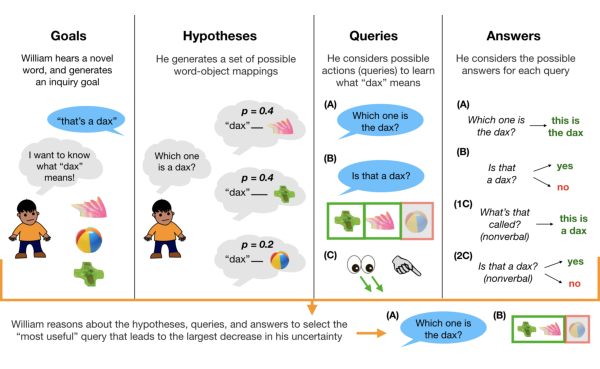
\includegraphics[width=0.9\linewidth]{erica_yoon_dissertation_files/figure-latex/word-learn-schematic-1} 

}

\caption[Schematic of an active word learning context.]{Schematic of an active word learning context using the decomposition of Optimal Experiment Design. Social input (hearing a new word) triggers an inquiry goal. Then the learner considers potential hypotheses for the candidate word-object links, weighting each hypothesis by its prior probability. In this case, the learner thinks that the new word is less likely to refer to the familiar object BALL. Next, he considers possible queries (actions) and the potential outcomes of those actions. In the word learning context, the child must direct queries towards a social partner, which provides the learner with more possible queries: both verbal (questions) and nonverbal (eye gaze; pointing). If the learner selects the action to maximize expected utility, then he would ask the most informative question, which removes all uncertainty for the meaning of 'Dax' -- 'What's that called?' If he does select the relatively less informative action of asking about a single object, he would be unlikely to ask about the familiar object BALL since there is less information to be gained from this query based on his prior beliefs.}\label{fig:word-learn-schematic}
\end{figure}
Nelson, McKenzie, Cottrell, \& Sejnowski (2010) demonstrate the
usefulness of taking an OED approach for differentiating competing
theories of information seeking in adults' category learning. They
created an OED model of their task, which included the design choices
(what combination of features to show participants) and the relevant
behavioral hypotheses (the different theories of category learning).
They used the model to simulate the outcomes of using different stimulus
sets, and selected the stimuli for which the competing theories made
different predictions, and thus speeded the rate of learning from their
experiments.

Coenen, Nelson, \& Gureckis (2017) provide a thorough review of the OED
framework and its links to human information seeking. They describe the
four parts of an OED model, which are necessary to compute the expected
value of an action: (1) hypotheses, (2) queries, (3) a generative model
of the types of answers that each query could elicit, and (4) a way to
score each answer with respect to the learning goal. There are also two
components that are external to the utility computation but important
for an account of human inquiry. First, having a learning goal, which
instantiates the process of reasoning about hypotheses, questions, and
answers. And second, having a stopping rule, which refers to a threshold
that causes the learner to stop seeking information and generate an
action. In Part III, I define each component of the OED model, and in
the Appendix for this chapter I provide the mathematical details of the
OED account.

\subsection{Evidence of OED-like reasoning in human
behavior}\label{evidence-of-oed-like-reasoning-in-human-behavior}

A growing body of psychological research has used the OED framework as a
metaphor for active learning. The proposal is that when people make
decisions, they engage in a similar process of evaluating the usefulness
of different actions relative to their learning goals. Using this
evaluation process, learners can then select behaviors that maximize the
potential for gaining information. One of the successes of the OED
account is that it can capture a wide range of information seeking
behaviors, including verbal question asking (Ruggeri \& Lombrozo, 2015),
planning interventions in causal learning tasks (C. Cook, Goodman, \&
Schulz, 2011), and decisions about where to look during scene
understanding (Najemnik \& Geisler, 2005).
(Figure~\ref{fig:word-learn-schematic} shows a schematic overview of how
OED principles shape the learning process for the task of word
learning.)

One compelling example of OED-like behavior is Nelson (2005)`s study of
eye movements during concept learning. Their model combined Bayesian
probabilistic learning, which represents current knowledge as a
probability distribution over concepts, with an OED model that
calculated the usefulness of different patterns of eye movements for the
goal of learning about the novel concepts. Nelson (2005) showed that an
OED model could predict a shift in participants' distribution of visual
fixations as they became more familiar with the target concepts. Early
in learning, when the concepts were unfamiliar, the model generated a
broader, less efficient distribution of fixations to explore all
candidate features. However, after the model began to learn the target
concepts, eye movement patterns shifted to become more efficient and
focused on a single stimulus dimension to maximize accuracy. This shift
from exploratory to efficient eye movements matched adult performance,
suggesting that human information seeking was well-adapted to the
structure of the learning problem and the uncertainty in the task.

Developmental work has also used OED models to ask whether children are
capable of selecting useful behaviors that maximize learning goals. For
example, Legare, Mills, Souza, Plummer, \& Yasskin (2013) found that 4-
to 6-year-old children consistently asked yes/no questions to figure out
the identity of an object hidden in a box. Children produced a high
proportion of questions that generated useful, constraining information
(e.g., ``Is it red?'') as opposed to questions that provided redundant
information (see also Mills, Legare, Grant, \& Landrum (2011); Mills,
Legare, Bills, \& Mejias (2010)). Moreover, children can generate
efficient actions to learn about the causal structure of objects. For
example, C. Cook et al. (2011) found that preschoolers could design
useful tests that successfully distinguished between competing
hypotheses for how to activate a music box, even showing the capacity to
reason about a decision that would influence future learning
opportunities.

Although the OED approach provides a formal account of information
seeking behaviors, there are several ways in which it falls short as an
explanation of self-directed learning. Coenen et al. (2017) argue that
OED models make several critical assumptions about the learner and the
learning task, including (1) the hypotheses/questions/answers under
consideration, (2) that people are actually engaging in some expected
utility computation in order to maximize the goal of knowledge
acquisition, and (3) that the learner has sufficient cognitive
capacities to carry out the calculations.

In the next section, I argue that the limitations of the OED approach
can be productively reconstrued as opportunities for understanding how
learning from other people could scaffold children's active learning. I
focus on integrating research and theory on social learning with the
five critical components of the OED model: goals, hypotheses, questions,
answers, and stopping rules (see Figure~\ref{fig:integrative-schematic}
for a schematic overview of the active-social learning account).

\hypertarget{active_social}{\section{Part III: Information seeking
within social contexts}\label{active_social}}

Why connect active learning processes with social learning effects?
First, children do not re-invent knowledge of the world, and while they
can learn a tremendous amount from their actions, much of their
generalization and abstraction is shaped by input from other people.
Moreover, social learning can be the only way to learn something (e.g.,
first language acquisition). Finally, children are often surrounded by
parents, other adults, and older peers -- all of whom may know more
about the world than they do, creating contexts where the opportunity
for social learning is ubiquitous.

Second, there is a body of empirical work showing that active learning
can be biased and ineffective in systematic ways. For example, work by
Klahr \& Nigam (2004) found that elementary school-aged children were
less effective at discovering the principles of well-controlled
experiments from their self-directed learning, but were capable of
learning these principles from direct instruction. D. B. Markant \&
Gureckis (2014) showed that active exploration provided no benefit over
passive input in category learning when there was a mismatch between the
target concept and adults' prior hypotheses going into the learning
task. And McCormack, Bramley, Frosch, Patrick, \& Lagnado (2016) found
that 6-7 year-olds showed no benefit from active interventions on a
causal system compared to observing another person perform the
interventions.

In a comprehensive review of the self-directed learning literature,
Gureckis \& Markant (2012) point out the learner's understanding of the
task determines the quality of active exploration: if the representation
is weak, then self-directed learning will be biased and ineffective.
Coenen et al. (2017) pursue this line of argument even further,
proposing a set of specific challenges for research on active learning.
Here is a sample of those open questions that are most relevant to the
ideas in this chapter:
\begin{itemize}
\tightlist
\item
  What triggers inquiry behaviors in the first place?
\item
  How do people construct a set of hypotheses?
\item
  How do people generate a set of queries?
\item
  What makes an answer good?
\item
  How do people generate and weight possible answers to their queries?
\item
  How does learning from answers affect query selection and belief
  change?
\end{itemize}
\noindent
In this section, I argue that ideas from research on social learning can
address these challenges. I start with the OED model and use it as a
conceptual tool to integrate social contexts and active learning. The
contribution of this formalization is that it makes the different
components of active learning explicit while highlighting the aspects
that might be particularly challenging for young learners. Moreover, the
``challenges'' to the OED account can be reconstrued as opportunities
for understanding the benefits of learning from other people. In each of
the following sub-sections, I define the challenge for active learning,
discuss how social contexts could address it, and highlight prior or
future empirical work that connects active and social learning accounts.
\begin{figure}[!t]

{\centering 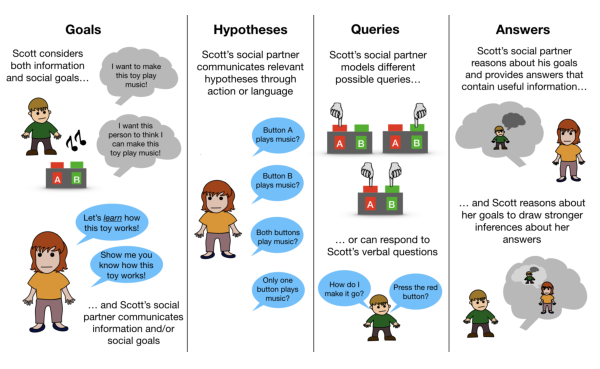
\includegraphics[width=0.9\linewidth]{erica_yoon_dissertation_files/figure-latex/integrative-schematic-1} 

}

\caption[Schematic of the integrative account of active learning within a social context.]{Schematic of active learning within a social context. Each panel shows how social information could influence a different component of the active learning process. These social effects occur in-the-moment of learning or over developmental time. Also, the cause of the social effect varies from the mere presence of another person to triggering a sophisticated psychological reasoning process about others' goal-directed behaviors. Note that the panels correspond to the different sub-sections in Part III of this chapter.}\label{fig:integrative-schematic}
\end{figure}
\subsection{Goals}\label{goals}

In the OED framework, an inquiry goal refers to the underlying
motivation for information seeking. Researchers often operationalize
these goals as a search for the target hypothesis amongst a set of
candidate hypotheses. Some examples of inquiry goals that children might
hold are:
\begin{itemize}
\tightlist
\item
  What is this speaker referring to? (word learning)
\item
  What types of objects are called ``daxes?'' (category learning)
\item
  How does this toy work? (causal learning)
\item
  Is this person reliable? (selective learning)
\end{itemize}
\noindent
Specifying learning goals is essential since without them the learner
will struggle to evaluate whether an action leads to progress. Coenen et
al. (2017) illustrate this point by saying,
\begin{quote}
The importance of such goals is made clear by the fact that in
experiments designed to evaluate OED principles, participants are
usually instructed on the goal of a task and are often incentivized by
some monetary reward tied to achieving that goal. Similarly, in
developmental studies, children are often explicitly asked to answer
specific questions, solve a particular problem, or choose between a set
of actions. (p.~32-33)
\end{quote}
\noindent
Characterizing children's goals, however, is not trivial since they
could consider a range of goals at any moment with no guarantee that
learning progress is one of them. One line of theorizing about the OED
hypothesis argues that useful information seeking should only occur in
the presence of precise tasks and goals. Consider the example of a
parent handing their child a new toy with several buttons on it and
saying, ``Let's figure out how this toy works!'' In this case, it
becomes possible to ask whether the child selects actions that are more
or less useful for increasing their knowledge of the toy's causal
structure.

This example illustrates how other people can trigger learning goals.
Empirical work shows how the actions of a social partner can increase
children's tendency to detect their uncertainty (see Lyons \& Ghetti
(2010) for a review). The upshot of this research is that children's
ability to realize when they do not know something is relatively slow to
develop. For example, Markman (1979) showed that elementary school-aged
children were unable to detect apparent inconsistencies in written
paragraphs (e.g., ``fish can't see without light, and there's no light
at the bottom of the ocean, but some fish at the bottom of the ocean
only know their food by its color.''). Interestingly, if the
experimenter gave children an explicit warning or challenge to find a
problem with the essay, then they were more likely to monitor their
uncertainty and asked more clarifying questions. This finding can be
reconstrued as an effect of the social context, shifting children's
expectations, highlighting the learning goal, and facilitating their
information seeking actions. Converging evidence comes Kim, Paulus,
Sodian, \& Proust (2016), who showed that 3- to 4-year-olds are more
likely to monitor their uncertainty about the contents of an opaque box
when they were told that they would have to teach another person about
the contents of the box (see also Lombrozo (2006)). In this case, the
anticipation of social interaction may have increased children's
tendency to focus on their goal to learn the identity of the objects.

In addition to triggering inquiry goals, social partners can directly
communicate the \emph{value} of learning goals relative to the other
goals that children may pursue. This connection draws on theoretical and
empirical work exploring how children's environments can shape their
intuitive frameworks for processing information and generating goals
(Dweck \& Leggett, 1988). Under these accounts, children's beliefs about
the malleability of traits influence whether they focus on taking
actions that increase their competence (prioritize learning) or that
demonstrate their fixed abilities (prioritize performing). Empirical
work shows that when adults use language to emphasize a learning goal
(e.g., ``If you pick the task in this box, you'll probably learn a lot
of new things.'' vs. ``If you pick this box, although you won't learn
new things, it will really show me what kids can do.''), then children
tend to select the more difficult task {[}elliott1988goals{]}. Moreover,
both lab-based experiments and observational work provide evidence that
the language adults use when praising children influences their tendency
to adopt inquiry goals (Cimpian, Arce, Markman, \& Dweck, 2007;
Gunderson et al., 2013).

While social partners can emphasize learning, the presence of another
person can also engage learners' psychological reasoning about their
mental states. This reasoning process can then elicit social goals that
take priority over learning goals. Consider the ``Goals'' panel of the
schematic active-social learning context shown in
Figure~\ref{fig:integrative-schematic}. If the learner is worried about
what his social partner thinks of him, then he might prioritize actions
that reduce the chance of appearing unknowledgeable and choose not to
ask about the novel objects. Moreover, he could seek out easy tasks that
demonstrate his competence at the expense of selecting actions that help
him learn. The OED framework typically focuses on informational goals
with progress measured as a reduction in uncertainty over candidate
hypotheses. However, recent empirical and modeling work has begun to
move beyond information-specific utility functions to include other
goals that learners may hold (e.g., saving time, money, or cognitive
resources) {[}meder2012information{]}.

Recent work in modeling pragmatic communication\footnote{Rational Speech
  Act (RSA) framework for pragmatic reasoning. The RSA approach models
  language comprehension and production as, ``a process of recursive
  reasoning about what speakers would have said, given a set of
  communicative goals'' (p.819) (Goodman \& Frank, 2016)} provides a way
to integrate social goals within the OED framework. For example, E. J.
Yoon, Tessler, Goodman, \& Frank (2017) modeled speakers' decisions to
use polite speech as opposed to direct speech (e.g., indirect language
such as ``we don't think that dress looks phenomenal on you'' as opposed
to ``It looks terrible'') as a tradeoff between maximizing informational
and social goals, showing that speakers are balancing these two when
deciding what to say.

In both OED and RSA, people are assumed to select actions that maximize
utility, but the politeness model allows social information to play a
role in the utility computation. Future research could adapt this
utility-theoretic approach and model the effects of social contexts as
changes to the weight children place on social goals, which, in turn,
leads to selecting easier tasks where they can appear competent (see E.
J. Yoon, MacDonald, Asaba, Gweon, \& Frank (2018) for an example of this
type of approach). This integration builds on the goal-orienting
accounts reviewed above (Dweck \& Leggett, 1988) since behavior is as an
output of a mixture of goals as opposed to children holding either a
performance or a learning goal.

Another open question about learning goals is how often children
experience contexts where these goals are apparent or emphasized in
their everyday experience. We do not yet have a reliable estimate of the
prevalence of situations that would lead children to generate learning
goals. One exception, however, is research on \emph{guided
participation} by Rogoff et al. (1993) provides evidence that parents
from a diverse set of cultural backgrounds produce high rates of
structuring and goal-orienting behaviors during activities such as
cooking, shopping, or working. It is interesting to consider whether
variability in children's exposure to goal-orienting behaviors could
influence children's tendency to generate learning goals spontaneously.

\subsection{Hypotheses}\label{hypotheses}

Once children have a learning goal, the next step in the OED model is to
figure out what hypotheses to consider. Intuitively, a hypothesis is a
candidate explanation for how the world works. For example, consider the
schematic learning context shown in
Figure~\ref{fig:word-learn-schematic}. Here, the child might generate
the following hypotheses about the meaning of a new word ``Dax'': (1)
Dax = object A, (2) Dax = object B, or (3) Dax = object C.\footnote{This
  hypothesis space is simplified since it only considers the possibility
  of one-to-one word-object mappings and that the new word refers to the
  co-occurring visual context.}

The set of hypotheses under consideration is critical for quantifying
effective self-directed learning in the OED account. The usefulness
function of expected information gain (see Appendix A for details) works
by comparing the learner's uncertainty over hypotheses before and after
they see an answer. Without a defined hypothesis space, however, it is
challenging to select the best action to reduce uncertainty. Put another
way; the OED framework does not readily deal with situations where
learners might have to consider a large space of hypotheses or might
perform actions without considering any hypotheses at all. These
challenges are especially relevant for developmental accounts that draw
on OED principles since these scenarios are plausible for young
learners. Social partners, however, can address this challenge by
providing children with a constrained set of hypotheses that facilitate
the comparison of different information-seeking actions.

Consider the case of children's early word learning where even the
simplest of words, concrete nouns, are often used in complex contexts
with multiple possible referents, which creates the potential for an (in
principle) unlimited number of hypotheses that children could entertain
when trying to figure out word meanings (Quine, 1960). Social-pragmatic
theories of lexical development often start from the idea that adults
constrain the learning task by providing social cues (e.g., eye gaze,
pointing) that connect words to their referents during labeling (P.
Bloom, 2002; E. V. Clark, 2009; Hollich et al., 2000). Some of our work
presented in Chapter 4 shows that the number and fidelity word-object
hypotheses that learners store tracks with the strength of social cues
available during the labeling moment (MacDonald, Yurovsky, \& Frank,
2017b). Other empirical work has found that children as young as 16
months prefer to map novel words to objects that are the target of a
speaker's gaze and not their own (D. A. Baldwin, 1993). And analyses of
naturalistic parent-child labeling events shows that young learners
tended to retain labels accompanied by clear referential cues, which
served to make a single object dominant in the visual field (Yu \&
Smith, 2012).

Social input can also shape the hypotheses that children generate by
revising their intuitive theories about the world. Gerstenberg \&
Tenenbaum (2017) describe an intuitive theory as, ``an ontology of
concepts, and a system of (causal) laws that govern how the different
concepts interrelate\ldots{}'' (p.~3). Importantly, these theories shape
how children interpret incoming information and, in turn, the set of
candidate explanations they could explore. Empirical work on conceptual
change across development has studied the ways that children integrate
input from other people with their current theories (Gelman, 2009). For
example, elementary school-aged children tend to hold a mixture of
beliefs about the shape of the earth, ranging from a flat earth theory
to the adult-like, sphere model (Vosniadou \& Brewer, 1992).
Interestingly, some children hold intermediate beliefs such as a theory
where there are two earths, suggesting that they actively integrate
aspects of their initial theory with the information they get from other
people (see Opfer \& Siegler (2004) for another example from intuitive
theories of biological concepts).

In sum, children's candidate hypotheses can be shaped by social
information. This effect can occur during the moment of learning (e.g.,
referential gaze during word learning) and over a developmental
timescale (e.g., intuitive theory revision). Critically, social partners
can facilitate active learning by constraining the set of hypotheses
under consideration, which makes comparing the utility of
information-seeking actions more tractable. An open question is how
children's information seeking changes as a function of the size of the
hypothesis space. Moreover, similar to the research on children's goals,
it would be useful to move beyond lab-based studies and towards
observational research that measures how children's everyday social
interactions constrain the hypotheses they decide to target with their
exploration behaviors.

\subsection{Queries}\label{queries}

Queries refer to the set of experiments that a scientist could conduct
to gather information about their hypotheses. In children's active
learning, queries are the set of actions they could take to collect
information from the world. Empirical work on active learning has
explored a variety of behaviors, including verbal questions, pushing a
button to figure out how a toy works, and decisions about where to look.
One of the strengths of the OED account is that it provides general
principles that could explain such a wide range of behaviors.

The challenge for young learners, however, is to discover what behaviors
are available and figure out which of those actions are useful for
learning. One way to address this challenge is for children to look to
older peers and adults to figure out what actions can help them learn.
Moreover, social learning contexts can change the space of possible
queries by adding the option of seeking information from a social
partner, which expands the set of possible learning-related actions
children could take.

Research on children's verbal questions provides insight into how social
partners could model useful queries. First, it is a truism that asking a
question in natural language requires that children have acquired a
conventionalized symbolic system, which must have been learned from
other people. Second, both experimental work and corpus analyses provide
evidence that children's question-asking becomes more varied and
productive over the first years of life as they get exposed to more
complex language input. Finally, observational studies have found that
that parents' use of wh-questions predicts children's later vocabulary
and verbal reasoning outcomes (Rowe, Leech, \& Cabrera, 2017), and
children of parents who were trained to ask ``good'' questions during
book reading episodes at home had children who asked better questions
during book reading sessions at school (Birbili \& Karagiorgou, 2009).
One explanation for these associations is that wh-questions led children
to produce more complex responses that build verbal abilities. Another
intriguing causal pathway, however, is that the frequency and type of
parents' questions provided children with a template for how to ask
useful questions.

Even if children can generate a set of queries, they still have to
evaluate the relative usefulness of each action concerning their
learning goal. Empirical work with adults shows a substantial gap
between people's question-generating and question-evaluation skills. For
example, Rothe, Lake, \& Gureckis (2015) used an OED model to measure
the expected information gain of adults' natural language questions in a
modified ``Battleship'' game and found that people rarely produced high
information gain questions. In a follow-up experiment, however, Rothe et
al. (2015) showed that when a different group of adults had access to
the list of questions generated by the participants in the unconstrained
version, they were quite good at recognizing questions that would
generate useful information.

Developmental work provides additional evidence of this
production-comprehension asymmetry in question asking. For example,
children younger than the age of three have difficulty generating useful
verbal questions compared to their older peers in lab-based experiments
(Mills et al., 2010, 2011), but even the youngest children in those
studies are capable of comprehending information elicited by others'
questions to succeed at parallel tasks (Mills, Danovitch, Grant, \&
Elashi, 2012). Moreover, Mills et al. (2011) manipulated whether
children were pre-exposed to adults who modeled useful queries and found
that this led to even the youngest children producing useful questions
at a much higher rate. Finally, converging evidence comes from research
showing that direct instruction (i.e., understanding the objectives of
inquiry and identifying useful questions) is necessary for
elementary-school-aged children to develop skill in designing
informative experiments for learning about physics concepts (Kuhn \&
Pease, 2008).

In addition to providing a model of queries, social contexts also expand
the set of possible questions by adding a social target for information
seeking actions. That is, the child has an additional choice: to gather
information from the non-social world or other people. The ``Questions''
panel in Figure 3 shows a child playing with a set of concrete objects.
If there is no social partner present, they could still interact with
the objects to learn about their shape, texture, or functional
properties. If another person is present, however, the child now has the
option to ask verbal questions or to seek information from the other
speaker by gathering their nonverbal cues (e.g., pointing, eye gaze, or
facial expressions).

Recent empirical work has explored the factors that influence children's
decisions to seek information from other people. For example, Fitneva,
Lam, \& Dunfield (2013) showed that children know when to query other
people to gain information that they could not get on their own (e.g.,
invisible properties of a novel social category). Additional evidence
comes from work by Lockhart, Goddu, Smith, \& Keil (2016) where they
showed that 5- to 11-year-olds could reliably determine the kinds of
things a person ``growing up on their own'' could learn from personal
experience (that the sky is blue) vs.~required interactions with other
people (that the earth is round). Finally, work on children's
help-seeking behaviors shows that both preschoolers and even infants
seek help systematically when completing a task, turning to a social
target to request information or acting on the world depending on which
information source was more likely to help them achieve their current
goal (Gweon \& Schulz, 2011; Vredenburgh \& Kushnir, 2016).

Some of our work has investigated how the presence of a social partner
changes the set of information seeking behaviors available to the
learner (see Chapter 3). By measuring changes in children's eye
movements during familiar language processing, we asked how real-time
information seeking adapts to support comprehension. We found that
children who were learning a visual-manual language gathered more
information before generating a language-driven gaze shift away from a
signer as compared to children processing spoken language while fixating
on a speaker (MacDonald, Blonder, Marchman, Fernald, \& Frank, 2017a).
This result suggests that sign language learners were sensitive to the
higher value of fixations in a visual-manual language where disengaging
from the signer reduces access to any following linguistic information.
We found a similar adaptation of information seeking in both children
and adults' processing of spoken language within noisy acoustic
environments where looking to a speaker's face provided visual
information that could support the comprehension of the less reliable
acoustic signal. Critically, listeners would not have had access to this
information seeking action outside of a face-to-face, social interaction
(e.g., listening to a noisy audio recording).

\subsection{Answers}\label{answers}

Once the learner generates a set of possible queries, they can simulate
the set of possible answers they could get in return. In the OED
framework, an answer is useful if it decreases the learner's uncertainty
about their hypotheses. The challenge for the child as an active learner
is two-fold: (1) figure out what which answers are likely for each query
and (2) decide how much to update their beliefs after seeing an answer.
In this section, I discuss how social contexts can affect each component
of the answer-evaluation process.

Defining a ``good'' answer is challenging. Intuitively, a good answer
provides the learner with information that they did not already know,
that they were interested in learning, and that is likely to be useful
beyond the current context. Even within the formal OED framework, there
have been a variety of ways to instantiate this utility function (e.g.,
information gain, probability gain, and Kullback-Leibler divergence)
(Nelson, 2005). These information-theoretic utility functions take into
account the learner's prior beliefs, which are represented as
probability distributions over hypotheses and compute the effect of each
answer on the learner's beliefs represented as a conditional probability
distribution.

Social learning theories often start from the idea that interactions
with other people increase the probability of getting useful
information. For example, evolutionary models argue that knowledge
transfer between generations allows for the gradual accumulation of
small improvements that eventually led to sophisticated tools, beliefs,
and practices that would be difficult, if not impossible, for any
individual to discover on their own (Kline, 2015). Boyd et al. (2011)
provide the example of a hunter stumbling across the link between the
color/texture of ice and its stability, saying that this type of rare
information would be much harder for individuals to re-discover on their
own. However, cultural transmission allows humans to pass these
discoveries down to subsequent generations, allowing humans to move
beyond the information that the world is likely to provide.

Csibra \& Gergely (2009)'s theory of ``Natural Pedagogy'' argues that an
assumption of \emph{generalizability} is a fundamental component of the
answers that children get when they interact with adults. Under their
account, when adults provide ostensive cues (eye gaze or child-directed
speech) to signal generalizable knowledge children update their beliefs
differently. Empirical work shows that infants are more likely to
generalize the valence of an object to a new person when learning in the
presence of an ostensive, pedagogical cue (Gergely, Egyed, \& Király,
2007). Moreover, infants are more likely to encode the stable features
of an object, as opposed to its location in space, if a communicative
signal such as a point guided their attention to that object (J. M. Yoon
et al., 2008).

In addition to an increased chance of seeing generalizable information,
features of the social context can also modulate the way active learners
evaluate possible answers. This link is one of the more developed
connections between the OED and social learning accounts. That is,
researchers have made progress in modeling the influence of different
assumptions that a learner could make about the process through which
other people generate answers. Shafto et al. (2012b) describe these
different sampling assumptions, placing them along a continuum that
varies regarding how much a learner should update their beliefs:
\begin{itemize}
\tightlist
\item
  \emph{Weak sampling}: answers generated at random from the set of all
  possible answers (independent of target hypothesis)
\item
  \emph{Strong sampling}: answers generated at random from the set of
  answers that are true of the correct hypothesis (linked to target
  hypothesis)
\item
  \emph{Pedagogical sampling}: answers generated that maximize the
  learner's belief in the correct hypothesis (linked to target
  hypothesis and consider alternative hypotheses)
\end{itemize}
\noindent
If the learner assumes strong or pedagogical sampling, then they can
make stronger inferences that speed learning. For example, if we see
someone press two buttons to activate a device, we are more likely to
think that both buttons were necessary if that person knew how the
machine worked and wanted to communicate to us how it worked. Otherwise,
if one of the buttons would have been sufficient, then it would not make
sense for them to perform the less efficient action of pressing both
buttons. The effects of these sampling assumptions are fundamentally
psychological. They require the learner to reason about others' goals
and to reason about whether other people are thinking about their
intentions. (See the ``Answers'' panel of
Figure~\ref{fig:integrative-schematic} for an illustration of this
recursive reasoning process within an active learning context.)

Empirical support for the pedagogical sampling account comes from a
range of domains/tasks, including word learning (Frank et al., 2009),
pragmatic inference (Frank \& Goodman, 2012), and causal reasoning
(Bonawitz et al., 2011). These empirical findings connect directly to
the OED model. Consider Xu \& Tenenbaum (2007a)'s finding that when a
knowledgeable teacher generates object labels, learners assumed the
examples indicated the true word meaning, making it more likely that the
teacher would draw three samples from the broader, basic category (as
opposed to the smaller subordinate category). They modeled this effect
by modifying the likelihood function in a Bayesian cognitive model. In
this case, the likelihood function for the teacher-driven condition was
designed to capture the idea that learners should prefer more
restrictive hypotheses if they are confident that the teacher generated
labels based on the actual word meaning. This formalization makes direct
contact with the OED model of human inquiry since learners consider how
much answers will update their beliefs, capturing the idea that
responses generated with the goal to teach carry more information.

Another line of empirical work has focused on children's decisions about
whom to learn from. Even young infants are capable of \emph{selective}
learning, rejecting answers that conflict with their knowledge (Pea,
1982) and seeking information from people who tend to provide useful
information in the past (Koenig, Clement, \& Harris, 2004). For example,
Chow, Poulin-Dubois, \& Lewis (2008) found that 14-month-olds are less
likely to follow the gaze of a person who had consistently directed gaze
towards an empty location. Moreover, children prefer to learn from
familiar rather than unfamiliar adults (Corriveau \& Harris, 2009),
adults rather than peers (Rakoczy, Hamann, Warneken, \& Tomasello,
2010), and ingroup rather than outgroup members (MacDonald, Schug,
Chase, \& Barth, 2013). Moreover, Gweon, Pelton, Konopka, \& Schulz
(2014) found that 14-month-olds explore objects more after interacting
with a teacher who had been under-informative in their previous
demonstrations, providing evidence of an early ability to link the
quality of answers to active learning decisions.

Interestingly, the outcome measures in these studies of selective
learning -- whom to direct questions towards or how long to explore a
novel toy -- are information-gathering decisions. While this is an
implicit link to the OED account, researchers have modeled selective
learning phenomena as modifications to the likelihood function in
Bayesian cognitive models. For example, Shafto et al. (2012a) developed
a model in which children reason about both the helpfulness and
knowledgeability of speakers when deciding whom to learn from and were
able to capture several qualitative findings from the selective trust
literature. This approach parallels the word learning and pedagogical
sampling models reviewed above, highlighting how social reasoning could
change the utility of the answers learners get from other people.

One candidate for future research is to ask how social contexts change
children's decisions about whether to initiate information seeking
behaviors in the first place. That is, if their social partners are
unlikely to provide useful answers, then active learning (even if
children are capable of selecting informative actions) becomes less
valuable. The dual consideration of costs and benefits in active
learning has been the focus of much research in machine learning, which
tries to select the set of questions to ask taking into account how long
it will take a human to respond (Haertel, Seppi, Ringger, \& Carroll,
2008). Moreover, recent lab-based studies and theorizing in social
cognition suggest that children are capable of ``intuitive utility
maximization'' reasoning that others take actions to increase rewards
while minimizing costs regarding time and effort (Jara-Ettinger, Gweon,
Tenenbaum, \& Schulz, 2015). It would be interesting to bring these
cost-based approaches to bear on questions about how social contexts
modify children's active learning.

\subsection{Stopping rules}\label{stopping-rules}

A stopping rule is a threshold that when exceeded causes the learner to
stop gathering information and generate a response. These rules fall
into two categories: information or time-based. For example, when
searching for information on the internet, a learner might create the
time-based stopping rule -- spend one hour searching -- or the
information-based rule -- explore until we find the definitions that we
need. The function of a stopping rule is to balance information gained
with reducing unnecessary time/effort put into the search task.

The challenge for both the child as active learner and researchers
interested in explaining stopping rules is both operationalizing and
estimating the critical pieces needed for developing a stopping rule:
the rate of information gain and the cost of information search. To
address this challenge, researchers have used ideas from theories of
animal foraging to model adults' decisions of when to stop gathering
information (Pirolli \& Card, 1999). For example, Manohar \& Husain
(2013) used a ``patch'' model to explain the timing of adults' decisions
about when to fixate and re-fixate on one of two symbolic gambles
displayed on a computer monitor. They proposed that fixating on an item
results in a leaky gain in precision and that people should shift their
gaze once their information gain rate falls below a pre-defined
threshold (see also Hills, Jones, \& Todd (2012) for evidence from
semantic memory). Moreover, much progress has been made by modeling
perceptual decisions as a noisy evidence accumulation process with
responses generated when information crosses a pre-defined threshold
(Ratcliff \& McKoon, 2008).

Social partners play a key role in children's decisions to stop
information seeking since they are a valuable resource of information.
Empirical work has primarily focused on how children persist in seeking
information from social partners if their initial request is not
satisfied. For example, Frazier, Gelman, \& Wellman (2009) used a corpus
analysis of parent responses to children's \emph{how} and \emph{why}
questions and found that preschoolers were more than twice as likely to
re-ask a question after getting a non-explanatory response (e.g., CHILD:
``Why you put yogurt in there?'' ADULT: ``Yogurt's part of the
ingredients'') compared to an explanatory answer (e.g., CHILD: ``How do
you get sick?'' ADULT: ``we don't know.'') (see also Deborah, Louisa
Chan, \& Holt (2004)). These studies suggest that even toddlers are
sensitive to when they have gathered sufficient information to address
their information seeking goals within social contexts.

In addition to providing information, social partners can take actions
that shape children's decisions about whether to persist in exploration.
For example, Bonawitz et al. (2011) showed that preschoolers spend less
time exploring an object and are less likely to discover alternative
object-functions after an adult explicitly taught a single function
(Bonawitz et al., 2011). Children's stopping behavior is reasonable
since their social partner communicated that there was no other
information to be gained by taking actions on the object. Moreover,
Butler \& Markman (2012) showed that an adults' pedagogical
demonstration led to an increase in children's object exploration when
testing whether a hidden property (magnetism) generalized to a new but
similar looking object. These results highlight the complex ways social
interactions can modulate children's thresholds for ending their
information search.

Our work exploring where children choose to look during real-time
language comprehension (see Chapter 3) can be construed as an effect of
access to social information on children's stopping decisions
(MacDonald, Marchman, Fernald, \& Frank, 2018). We found that both
adults and children fixate more on a speaker's face when processing
familiar words in a noisy auditory environment, an adaptation that
resulted in a higher proportion of gaze shifts to the named referent. We
used a cognitive model of decision making (Drift-Diffusion Model
Ratcliff \& McKoon (2008)) to provide evidence that an increase to
listeners' decision thresholds, and not processing efficiency, best
explained the behavioral results. This approach provides an example of
bringing cognitive models of decision making into contact with empirical
questions about children's language comprehension within face-to-face
social interactions.

Another promising approach for future research is to ask how children's
developing capacity to reason about the cost of actions changes their
active learning behaviors. In the OED framework, cost (e.g., monetary
value of running an additional experiment) is critical to deciding when
to stop gathering additional information, but this is complex to
operationalize in human information seeking. However, there has also
been a growing interest in developing ``cost-sensitive'' active learning
algorithms in the field of machine learning (Haertel et al., 2008), with
researchers beginning to define costs in increasingly sophisticated
ways. For example, Settles, Craven, \& Friedland (2008) point out that
the cost of information gathering should not be measured as a reduction
in the number of training trials if those training trials vary in length
because specific questions are more challenging to answer.

An important next step to understanding children as efficient active
learners is to explore how they balance the desire want to ask questions
that maximize information gain while taking into account the cost
incurred by others (e.g., time or mental effort) to provide that
information. This idea is fundamentally psychological in that it expands
the utility computation to include some measure of how our behavior
affects others' actions and mental states. This line of research falls
directly out of an integrated active-social learning framework.

\section{Conclusions: Eye movements as a case
study}\label{conclusions-eye-movements-as-a-case-study}

In this chapter, I presented concrete definitions of active and social
learning and described a unifying framework of information seeking
within social learning contexts. I used Optimal Experiment Design (OED)
as a theoretical tool to propose that the presence of another person can
affect children's information seeking by:
\begin{enumerate}
\def\labelenumi{\arabic{enumi}.}
\tightlist
\item
  instantiating learning goals, communicating the value of learning
  goals, or triggering social goals
\item
  constraining the learner's hypothesis space
\item
  modeling useful queries
\item
  providing useful answers
\item
  changing thresholds for stopping information seeking
\end{enumerate}
\noindent
The account described in this chapter argues that the social and active
learning theories have much to be gained from considering the other.
Active learning accounts will benefit by understanding how learners
incorporate social information into their decision making, allowing
researchers to develop more sophisticated utility functions that might
better capture what people care about when learning something new. This
approach seems especially crucial for characterizing the development of
active learning since observational studies of children's learning
environments suggest that opportunities to learn from social interaction
are ubiquitous.

On the other hand, researchers interested in social learning phenomena
can benefit from advances in the study of active learning by connecting
their ideas to the rich traditions of machine learning, decision theory,
and statistics. Moreover, research on social learning phenomena often
uses information-seeking decisions as dependent variables in
experiments. Thus, a secondary benefit would be a better understanding
of the factors that influence the measurement of social learning
effects.

Finally, the evidence reviewed in this chapter shows that research has
mostly focused on lab-based experiments where social and active learning
effects are measured in isolation during highly-constrained tasks. An
important next step is to estimate the presence of learning goals,
tractable hypothesis spaces, and the quality of answers in children's
everyday experiences. This line of inquiry will require a shift from
relying on lab experiments to leveraging large-scale, observational
datasets. And while this approach adds complexity, I think that the
benefit will be a far greater understanding of how children's active
learning operates over fundamentally social input.

The rest of this thesis presents a series of empirical studies of
familiar language comprehension and novel word learning, which I situate
within the integrative framework discussed here. The majority of the
experiments use eye movements as a case study of children's early
information seeking. To motivate this choice, in the next secttion, I
briefly describe how eye movements could reflect different kinds of
information seeking, clarifying both the linking hypothesis and the set
of behaviors that the empirical work aims to address.

\subsection{Why eye movements?}\label{why-eye-movements}

There are several reasons why eye movements are well-suited for asking
questions about children's information seeking within social contexts.
First, deciding where to allocate visual attention is an
ecologically-valid component of early learning. That is, there are many
places that young children could be looking, and one of the fundamental
challenges for children is to focus their attentional resources on the
relevant aspects of the environment. Empirical work with infants has
shown that their attention is often stimulus-driven and sticky (Oakes,
2011), suggesting that young learners should benefit from using social
cues to guide their visual attention to relevant information. Moreover,
control over gaze is earlier to develop as compared to other, more
explicit forms of information seeking such as verbal question asking.
And the efficiency of children's gaze shifts rapidly develops during
early childhood (e.g., children's eye movement to seek out named objects
Fernald, Pinto, Swingley, Weinbergy, \& McRoberts (1998)). Together,
these findings suggest that active control over eye gaze is useful for
the ecological learning tasks that children face.

Visual fixations have also been successfully modeled as a form of
information seeking. In these frameworks, eye movements are
characterized as a way to gather information to reduce uncertainty and
guide future actions. For example, eye movements during an activity like
making a sandwich are best explained by people's task goals as opposed
to external features of the visual world such as the salience of objects
(Hayhoe \& Ballard, 2005). Moreover, changes in the distribution of
adults' gaze during category learning can be explained by an OED model
that calculates the usefulness of different types of fixations for the
goal of learning concepts (Nelson, 2005). These successes help to
clarify our hypothesis linking the observable behavior of gaze shifts to
the psychological construct of interest -- information seeking. This
link provides a foundation from which we can interpret the effects of
social context on information seeking eye movements.

Before presenting an overview of the empirical work, it is worth
highlighting two additional points about eye movements and information
seeking. First, multiple mechanisms can drive visual attention. Gottlieb
(2012) reviews evidence for three types of attention: Attention for
action, for learning, and for liking. Each of these mechanisms assigns
value to the information returned by an eye movement differently. Eye
movements for action will tend to cluster around areas that generate
highly reliable cues, whereas eye movements for learning will focus on
locations that are less predictable, and finally, fixations for liking
will be driven by the reward probability predicted by a visual cue. In
this dissertation, I focus on eye movements that gather information to
guide actions such as locating a named, familiar object in the visual
world or learning the mapping between a new label and an unfamiliar
object.

Second, theoretical work on goal-based vision has proposed two, broad
categories of information-seeking eye movements: (1) fixations that
gather task-related information such as frequently shifting gaze towards
the rear-view mirror while driving, and (2) eye movements that are used
to explore a new task environment without a specific information goal
(Henderson, Brockmole, Castelhano, \& Mack, 2007). Prior empirical work
has shown dissociations between these two systems of looking for action
and looking for learning at both the behavioral and neural levels of
analysis (Maddux \& Holland, 2011). Here, I focus on fixations that
gather information for a specific task, as opposed to more exploratory
fixations, which are better explained by models of information search
and curiosity-driven actions in which learners explore in an open-ended
fashion to discover new tasks (Baranes, Oudeyer, \& Gottlieb, 2015;
Gottlieb \& Oudeyer, 2018).

In the next section, I present an overview of the empirical work in the
dissertation, linking it to the integrative framework discussed in this
chapter. I also highlight the relevant pieces of the broader framework
that the empirical work addresses. Importantly, these case studies tend
to focus on eye movements that gather task-related information to guide
future action, as opposed to exploratory eye movements in a novel
environment. This feature makes them a good candidate for the
active-social framework inspired by OED since these models were
developed to explain information seeking in the context of well-defined
tasks and clear learning goals.

\subsection{Links between case studies and the broader
framework}\label{links-between-case-studies-and-the-broader-framework}

Chapter 2 investigates children's decisions about where to look while
comprehending a visual-manual language (American Sign Language: ASL). In
the grounded sign processing context, children must use visual fixations
to gather information about both the referents and the linguistic
signal, creating competition for visual attention that is not present in
spoken language comprehension. This competition could fundamentally
change how children decide to gather visual information during real-time
language comprehension. Using our active-social theoretical framework,
we might hypothesize that ASL-learners query the visual world in
different ways such as fixating longer on social partners before seeking
a named object since this behavior provides access to language, which
can help guide future actions. Alternatively, it could be that ASL
learners show parallel looking patterns to children acquiring spoken
language, shifting their gaze to gather visual information about the
objects in the scene soon after they have sufficient information about
the identity of the named object. Chapter 2 explores these questions by
measuring the timing and location of ASL learners' eye movements as they
process sentences that contain familiar signs referring to objects in
the visual scene.

Chapter 3 builds on the sign language work by directly comparing the
gaze dynamics of children learning ASL to children learning spoken
English during familiar language processing. We measure when children
decide to stop fixating on a social partner to seek named referents in
the visual world. Using our integrative framework, we hypothesized that
looking to a signer returns higher value information for the specific
task of identifying the named object, which would lead signers to
generate slower but more consistent gaze shifts away from the language
source and to the rest of the visual world. Chapter 3 also describes a
study of English-learning children and adult's eye movements in noisy
auditory contexts. We hypothesized that looking to a speaker becomes
more useful when the auditory signal is less reliable, which, as in the
ASL case, would make children fixate on the language source longer to
gather more information, leading them to produce more
language-consistent gaze shifts.

Chapters 4 and 5 explore how the information seeking framework
generalizes to processing words in the context of social cues to
reference. Social cues are an interesting test case for our
active-social account because communicative partners who produce
reliable cues to reference might become more valuable targets for
children's looking. Thus, we hypothesized that in the context of
reliable social cues, children should fixate longer on their social
partner, modulating the information stored from a labeling event. In
Chapter 4, we present a series of large-scale word learning experiments,
showing that the presence of a social cue reduces the number of
word-object hypotheses that adults remember from a labeling event.
Chapter 5 describes a set of eye-tracking studies that measure when
children decide to stop fixating on a social partner as a function of
(1) whether the social partner provides a cue to reference and (2) their
knowledge of the word-object mappings.

Overall, the goal of the empirical work is to ask how children's gaze
patterns adapt to a diverse set of contexts that change the value of
seeking information from social partners. The common thread across this
research is that children's real-time visual information seeking is
quite flexible and can adapt to the informational structure of the
environment to support language processing.

\chapter[Children's distribution of visual attention during real-time
American Sign Language comprehension]{\texorpdfstring{Children's
distribution of visual attention during real-time American Sign Language
comprehension\footnote{This chapter is published in MacDonald, LaMarr,
  Corina, Marchman, \& Fernald (2018). Real-time lexical comprehension
  in young children learning American Sign Language. \emph{Developmental
  science}, e12672.}}{Children's distribution of visual attention during real-time American Sign Language comprehension}}\label{childrens-distribution-of-visual-attention-during-real-time-american-sign-language-comprehension}

\chaptermark{Information seeking during ASL processing}

This chapter presents a study of eye movements in a visual-manual
language (American Sign Language: ASL). ASL is a compelling case because
children use visual fixation to gather information about referents and
the linguistic signal. In contrast, children learning spoken language
can look away from their social partners while still gathering more
linguistic information through the auditory channel. Within the broader
active-social framework, this study asks whether ASL-learners' visual
information seeking actions (i.e., queries) look dramatically different
given the constraints of processing a visual language in real time or by
having differential access to auditory information in day-to-day life.

To answer this question, we measured eye movements during real-time ASL
comprehension of 29 native ASL-learning children (16-53 mos, 16 deaf, 13
hearing) and 16 fluent deaf adult signers. All signers showed evidence
of incremental language comprehension, tending to initiate an eye
movement before sign offset. Moreover, Deaf and hearing ASL-learners
showed remarkably similar gaze patterns. Finally, variation in
children's ASL processing was positively correlated with age and
vocabulary size. These results suggest that, despite competition for
attention within a single modality, signers will use visual attention to
rapidly gather information about signs and seek named objects in ways
that parallel spoken language processing. Moreover, these results
suggest that the timing and accuracy of visual fixations in ASL reflect
language-relevant information processing skills.
\begin{figure}[!t]

{\centering 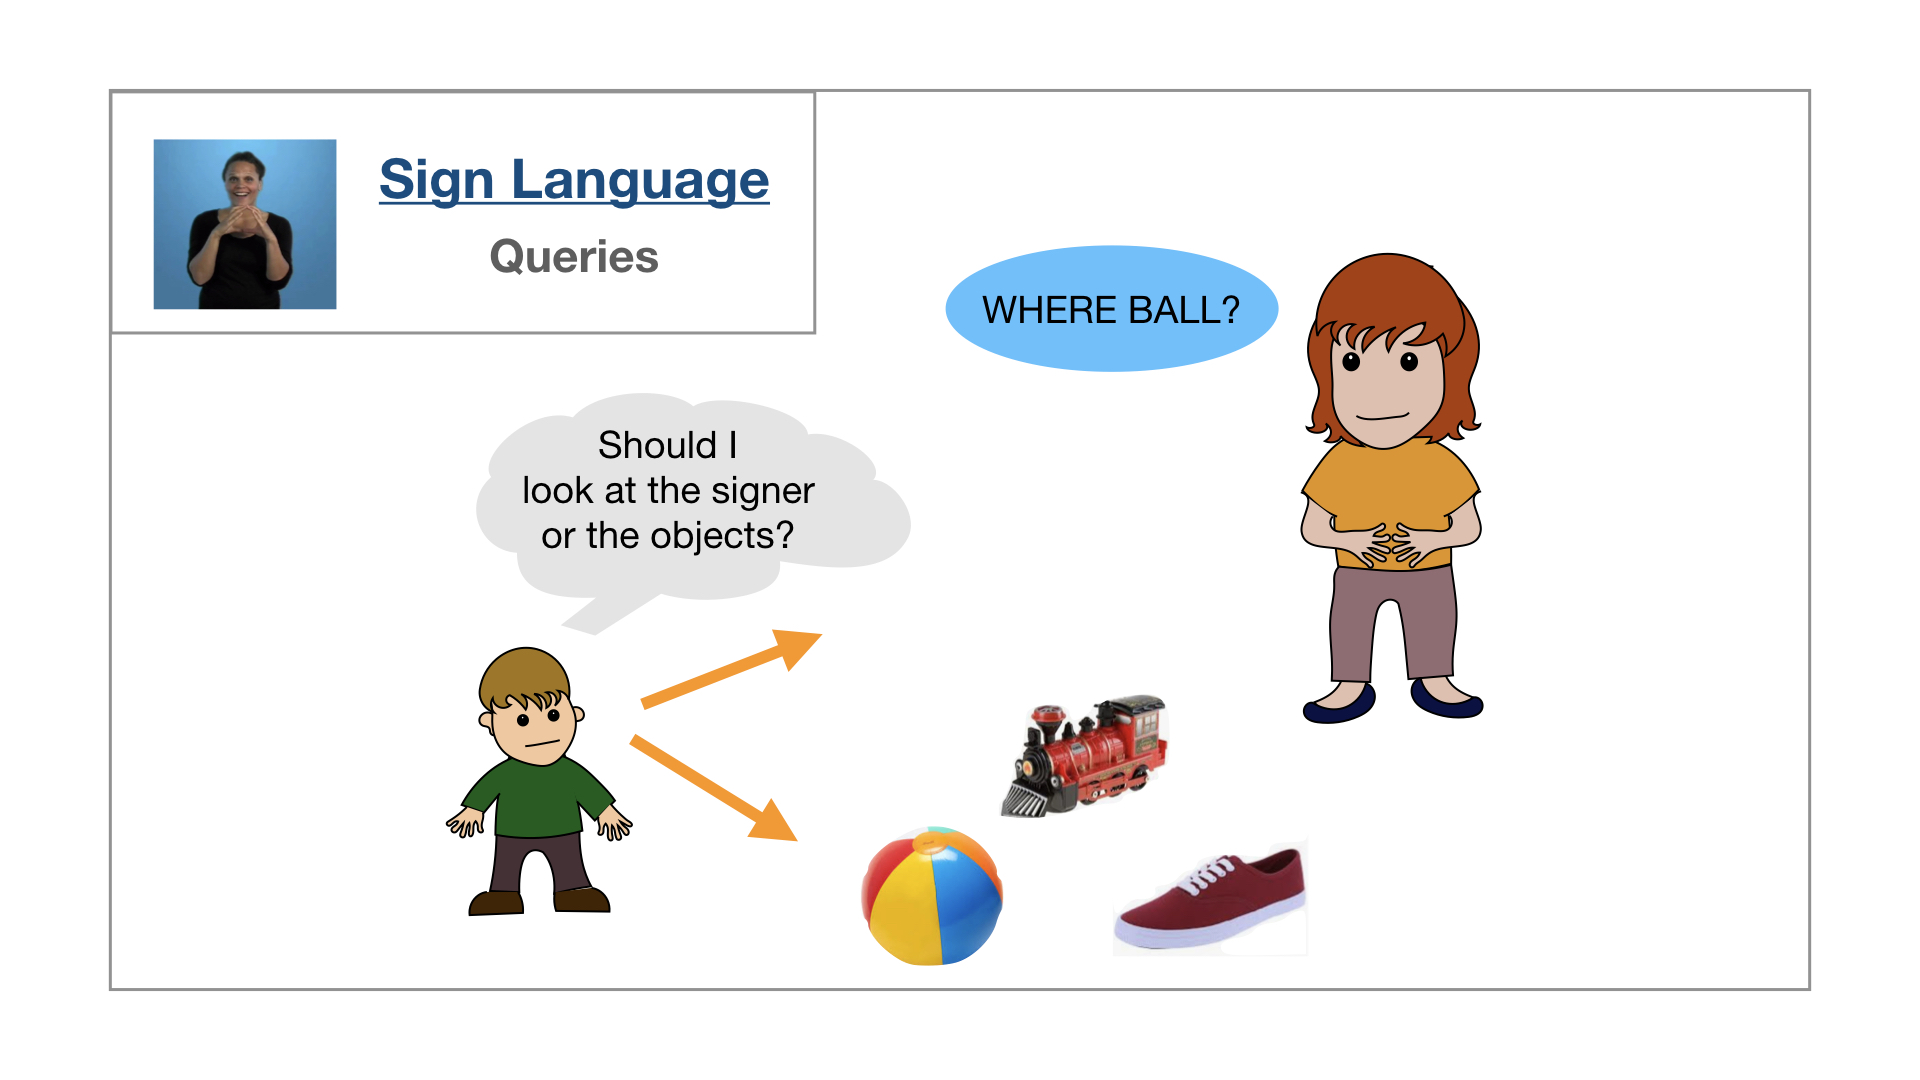
\includegraphics[width=0.9\linewidth]{/Users/ejyoon/Documents/Documents/Research/dissertation/index/chapter_child_rmds/SOL/figures/sol} 

}

\caption[Overview of Chapter 2.]{A schematic showing the components of the active-social learning framework addressed by the case study in Chapter 2.}\label{fig:schematic-sol}
\end{figure}
\section{Introduction}\label{introduction-1}

Finding meaning in a spoken or a signed language requires learning to
establish reference during real-time interaction -- relying on audition
to interpret spoken words, or on vision to interpret manual signs.
Starting in infancy, children learning spoken language make dramatic
gains in their efficiency in linking acoustic signals representing
lexical forms to objects in the visual world. Studies of spoken language
comprehension using the looking-while-listening (LWL) procedure have
tracked developmental gains in language processing efficiency by
measuring the timing and accuracy of young children's gaze shifts as
they look at familiar objects and listen to simple sentences (e.g.,
``Where's the ball?'') naming one of the objects (Fernald, Zangl,
Portillo, \& Marchman, 2008; Law \& Edwards, 2014; Venker, Eernisse,
Saffran, \& Ellis Weismer, 2013). Such research finds that eye movements
to named objects occur soon after the auditory information is sufficient
to enable referent identification, and often prior to the offset of the
spoken word (Allopenna, Magnuson, \& Tanenhaus, 1998). Moreover,
individual differences in the speed and accuracy of eye movements in
response to familiar words predict vocabulary growth and later language
and cognitive outcomes (Fernald, Perfors \& Marchman, 2006; Marchman \&
Fernald, 2008). Together, these results suggest that gaze shifts to
objects in response to spoken language reflect a rapid integration of
linguistic and visual information, and that variability in the timing of
these gaze shifts provides researchers a way to measure the efficiency
of the underlying integration process.

Much less is known about how language influences visual attention during
sign language comprehension, especially in young learners. Given the
many surface-level differences between signed and spoken languages, it
is not immediately clear whether the findings from spoken language will
generalize to signed languages or whether they are specific to
mechanisms of language comprehension in the auditory modality. In
particular, studies with children learning spoken languages find that
these skills undergo dramatic developmental changes over the 2nd and 3rd
years of life. Moreover, there are significant relations between
variation in efficiency in online language processing, as indexed by
language-driven eye movements, and measures of linguistic achievement,
such as vocabulary size and scores on standardized tests (Fernald et
al., 2006; Marchman \& Fernald, 2008). Will individual variation in
language processing among children learning a signed language also be
related to their age and vocabulary outcomes, as observed in children
learning a spoken language?

Here we address this question by developing precise measures of speed
and accuracy in real-time sign language comprehension by children
learning American Sign Language (ASL). First, we estimate the extent to
which adults and children tend to shift visual attention to a referent
and away from the language source prior to the offset of a sign naming
an object in the visual scene. Will signers wait until the end of the
signed utterance, perhaps to reduce the probability of missing upcoming
linguistic information? Or will signers shift gaze incrementally as the
signs unfold in time, initiating saccades soon after there is enough
information in the signal to identify the referent, similar to children
and adults processing spoken language? Another related possibility is
that signers would produce incremental gaze shifts to the named objects
while still monitoring the linguistic signal in the periphery. This
analysis provides an important first step towards validating the linking
hypothesis that eye movements generated in our task reflect efficiency
of sign recognition, rather than some other process, such as attending
to the objects after the process of sign comprehension is complete. If
children and adults produce rapid gaze shifts prior to target sign
offset, this would provide positive evidence of incremental ASL
processing.

Next, we compare the time course of ASL processing in deaf and hearing
native ASL-learners to ask whether having the potential to access
auditory information in their day-to-day lives would change the dynamics
of eye movements during ASL processing. Do deaf and hearing native
signers show parallel patterns of looking behavior driven by their
similar language background experiences and the in-the-moment
constraints of interpreting a sign language (i.e., fixating on a speaker
as a necessary requirement for gathering information about language)? Or
would the massive experience deaf children have in relying on vision to
monitor both the linguistic signal and the potential referents in the
visual world result in a qualitatively different pattern of performance
compared to hearing ASL learning, e.g., waiting until the end of the
sentence to disengage from the signer? This analysis is motivated by
prior work that has used comparisons between native hearing and deaf
signers to dissociate the effects of learning a visual-manual language
from the effects of lacking access to auditory information (e.g.,
Bavelier, Dye, \& Hauser, 2006).

Finally, we compare timing and accuracy of the eye movements of young
ASL-learners to those of adult signers, and ask whether there are
age-related increases in processing efficiency that parallel those found
in spoken languages. We also examine the links between variability in
children's ASL processing skills and their expressive vocabulary
development. A positive association between these two aspects of
language proficiency, as previously shown in children learning spoken
languages, provides important evidence that skill in lexical processing
efficiency is a language-general phenomenon that develops rapidly in
early childhood, regardless of language modality.

\subsection{ASL processing in adults}\label{asl-processing-in-adults}

Research with adults shows that language processing in signed and spoken
languages is similar in many ways. As in spoken language, sign
recognition is thought to unfold at both the lexical and sub-lexical
levels. Moreover, sign processing is influenced by both lexicality and
frequency; non-signs are identified more slowly than real signs (Corina
\& Emmorey, 1993) and high frequency signs are recognized faster than
low frequency signs (Carreiras, Gutiérrez-Sigut, Baquero, \& Corina,
2008). Recent work using eye-tracking methods found that adult signers
produce gaze shifts to phonological competitors, showing sensitivity to
sub-lexical features, and that these shifts were initiated prior to the
offset of the sign, showing evidence of incremental processing
(Lieberman, Borovsky, Hatrak, \& Mayberry, 2015). In addition, Caselli
and Cohen-Goldberg (2014) adapted a computational model, developed for
spoken language (Chen \& Mirman, 2012), to explain patterns of lexical
access in sign languages, suggesting that the languages share a common
processing architecture.

However, differences between spoken and signed languages in both
sub-lexical and surface features of lexical forms could affect the time
course of sign recognition (for reviews, see Carreiras, 2010 and Corina
\& Knapp, 2006). For example, Emmorey and Corina (1990) showed deaf
adults repeated video presentations of increasingly longer segments of
signs in isolation and asked them to identify the signs in an open-ended
response format. In the same study, English-speaking adults heard
repeated presentations of increasingly longer segments of spoken words.
Accurate identification of signs required seeing a smaller proportion of
the total sign length compared to words (see also Morford \& Carlsen,
2011), suggesting that features of visual-manual languages, such as
simultaneous presentation of phonological information, might increase
speed of sign recognition. Moreover, Gutierrez and colleagues (2012)
used EEG measures to provide evidence that semantic and phonological
information might be more tightly linked in the sign language lexicon
than in the spoken language lexicon. Thus there is evidence for both
similarities and dissimilarities in the processes underlying spoken-word
and manual-sign recognition. However, with a few exceptions
(e.g.~Lieberman et al., 2015, 2017), most of this work has relied on
offline methods that do not capture lexical processing as it unfolds in
time during naturalistic language comprehension. In addition, no
previous studies have characterized how young ASL-learners choose to
divide visual attention between a language source and the nonlinguistic
visual world during real-time language comprehension.

\subsection{Lexical development in
ASL}\label{lexical-development-in-asl}

Diary studies show that ASL acquisition follows a similar developmental
trajectory to that of spoken language (Lillo-Martin, 1999; Mayberry \&
Squires, 2006). For example, young signers typically produce
recognizable signs before the end of the first year and two-sign
sentences by their 2nd birthday (Newport \& Meier, 1985). And as in many
spoken languages (Waxman et al., 2013), young ASL-learners tend first to
learn more nouns than verbs or other predicates (Anderson \& Reilly,
2002).

However, because children learning ASL must rely on vision to process
linguistic information and to look at named objects, it is possible that
basic learning processes, such as the coordination of joint visual
attention, might differ in how they support lexical development (Harris
\& Mohay, 1997). For example, in a study of book reading in deaf and
hearing dyads, Lieberman, Hatrak, and Mayberry (2015) found that deaf
children frequently shifted gaze to caregivers in order to maintain
contact with the signed signal. Hearing children, in contrast, tended to
look continuously at the book, rarely shifting gaze while their
caregiver was speaking. This finding suggests that the modality of the
linguistic signal may affect how young language learners negotiate the
demands of processing a visual language while simultaneously trying to
fixate on the referents of that language.

This competition for visual attention in ASL could lead to qualitatively
different looking behavior during real-time ASL comprehension, making
the link between eye movements and efficiency of language comprehension
in ASL less transparent. On the one hand, demands of relying on vision
to monitor both the linguistic signal and the named referent might cause
signers to delay gaze shifts to named objects in the world until the end
of the target sign, or even the entire utterance. In this case, eye
movements would be less likely to reflect the rapid, incremental
influence of language on visual attention that is characteristic of
spoken language processing. Another possibility is that ASL-learners,
like spoken language learners, will shift visual attention as soon as
they have enough linguistic information to do so, producing saccades
prior to the offset of the target sign. Evidence for incremental
language processing would further predict that eye movements during ASL
processing could index individual differences in speed of incremental
comprehension, as previously shown in spoken languages.

\subsection{Research questions}\label{research-questions}

Adapting the LWL procedure for ASL enables us to address four questions.
First, to what extent do children and adult signers shift their gaze
away from the language source and to a named referent prior to the
offset of the target sign? Second, how do deaf and hearing ASL-learners
compare in the time course of real-time lexical processing? Third, how
do patterns of eye movements during real-time language comprehension in
ASL-learners compare to those of adult signers? Finally, are individual
differences in ASL-learners' processing skill related to age and to
expressive vocabulary development?

\section{Study}\label{study}

\subsection{Methods}\label{methods}

Participants were 29 native, deaf and hearing ASL-learning children (17
females, 12 males) and 16 fluent adult signers (all deaf), as shown in
Table 1. Since the goal of the current study was to document
developmental changes in processing efficiency in native ASL-learners,
we set strict inclusion criteria. The sample consisted of both deaf
children of deaf adults and hearing Children of Deaf Adults (CODAs),
across a similar age range. It is important to note that all children,
regardless of hearing status, were exposed to ASL from birth through
extensive interaction with at least one caregiver fluent in ASL and were
reported to experience at least 80\% ASL in their daily lives.
Twenty-five of the 29 children lived in households with two deaf
caregivers, both fluent in ASL. Although the hearing children could
access linguistic information in the auditory signal, we selected only
ASL-dominant learners who used ASL as their primary mode of
communication both within and outside the home (10 out of 13 hearing
children had two deaf caregivers). Adult participants were all deaf,
fluent signers who reported using ASL as their primary method of
communication on a daily basis. Thirteen of the 16 adults acquired ASL
from their parents and three learned ASL while at school.

Our final sample size was determined by our success over a two-year
funding period in recruiting and testing children who met our strict
inclusion criteria -- receiving primarily ASL language input. It is
important to note that native ASL-learners are a small population. The
incidence of deafness at birth in the US is less than .003\%, and only
10\% of the 2-3 per 1000 children born with hearing loss have a deaf
parent who is likely to be fluent in ASL (Mitchell \& Karchmer, 2004).
In addition to the 29 child participants who met our inclusion criteria
and contributed adequate data, we also recruited and tested 17 more
ASL-learning children who were not included in the analyses, either
because it was later determined that they did not meet our stringent
criterion of exposure to ASL from birth (n = 12), or because they did
not complete the real-time language assessment due to inattentiveness or
parental interference (n = 5).

\begingroup\fontsize{12}{14}\selectfont
\begin{longtable}[t]{lrrrrr}
\caption[Age of ASL-learning children]{\label{tab:sol-demo-table}Age (in months) of hearing and deaf ASL-learning participants}\\
\toprule
\textbf{Hearing status} & \textbf{n} & \textbf{Mean} & \textbf{SD} & \textbf{Min} & \textbf{Max}\\
\midrule
deaf & 16 & 28.0 & 7.5 & 16 & 42\\
hearing & 13 & 29.4 & 11.2 & 18 & 53\\
\hline
all children & 29 & 28.6 & 9.2 & 16 & 53\\
\bottomrule
\end{longtable}
\endgroup{}

\subsubsection{Measures}\label{measures}

Expressive vocabulary size: Parents completed a 90-item vocabulary
checklist, adapted from Anderson and Reilly (2002), and developed
specifically for this project to be appropriate for children between 1.5
and 4 years of age. Vocabulary size was computed as the number of signs
reported to be produced by the child.

ASL Processing: Efficiency in online comprehension was assessed using a
version of the LWL procedure adapted for ASL learners, which we call the
Visual Language Processing (VLP) task. The VLP task yields two measures
of language processing efficiency, reaction time (RT) and accuracy.
Since this was the first study to develop measures of online ASL
processing efficiency in children of this age, several important
modifications to the procedure were made, as described below.

\subsubsection{Procedure}\label{procedure}

The VLP task was presented on a MacBook Pro laptop connected to a 27''
monitor. The child sat on the caregiver's lap approximately 60 cm from
the screen, and the child's gaze was recorded using a digital camcorder
mounted behind the monitor. To minimize visual distractions, testing
occurred in a 5' x 5' booth with cloth sides. On each trial, pictures of
two familiar objects appeared on the screen, a target object
corresponding to the target noun, and a distracter object. All picture
pairs were matched for visual salience based on prior studies with
spoken language (Fernald et al., 2008). Between the two pictures was a
central video of an adult female signing the name of one of the
pictures. Participants saw 32 test trials with five filler trials (e.g.
``YOU LIKE PICTURES? MORE WANT?'') interspersed to maintain children's
interest.

Coding and Reliability. Participants' gaze patterns were video recorded
and later coded frame-by-frame at 33-ms resolution by highly-trained
coders blind to target side. On each trial, coders indicated whether the
eyes were fixated on the central signer, one of the images, shifting
between pictures, or away (off), yielding a high-resolution record of
eye movements aligned with target noun onset. Prior to coding, all
trials were pre-screened to exclude those few trials on which the
participant was inattentive or there was external interference. To
assess inter-coder reliability, 25\% of the videos were re-coded.
Agreement was scored at the level of individual frames of video and
averaged 98\% on these reliability assessments.

\subsubsection{Stimuli}\label{stimuli}

\emph{Linguistic stimuli.} To allow for generalization beyond
characteristics of a specific signer and sentence structure, we recorded
two separate sets of ASL stimuli. These were recorded with two native
ASL signers, using a different alternative grammatical ASL sentence
structures for asking questions (see Petronio and Lillo-Martin, 1997):
\begin{itemize}
\tightlist
\item
  Sentence-initial wh-phrase: ``HEY! WHERE {[}target noun{]}?''
\item
  Sentence-final wh-phrase: ``HEY! {[}target noun{]} WHERE?''
\end{itemize}
\noindent Each participant saw one stimulus set which consisted of one
ASL question structure, with roughly an even distribution of children
across the two stimulus sets (16 saw sentence-initial wh-phrase
structure; 13 saw the sentence-final wh-phrase structure).
\begin{table}

\caption[Iconicity scores and phonological overlap for ASL stimuli]{\label{tab:sol-asl-lex-table}Iconicity scores (1 = not iconic at all; 7 = very iconic) and degree of phonological overlap (out of 5 features) for each sign item-pair. Values were taken from ASL-LEX, a database of lexical and phonological properties of signs in ASL.}
\centering
\resizebox{\linewidth}{!}{
\begin{tabular}[t]{>{\raggedright\arraybackslash}p{3.5cm}>{\raggedleft\arraybackslash}p{3cm}l}
\toprule
\textbf{Item Pair (iconicity score 1-7)} & \textbf{Number of matched features} & \textbf{Matched features}\\
\midrule
bear (3.0) -- doll (1.2) & 1 & Movement\\
cat (4.6) -- bird (4.5) & 3 & Selected Fingers, Major Location, Sign Type\\
car (6.2) -- book (6.7) & 4 & Selected Fingers, Major Location, Movement, Sign Type\\
ball (5.7) -- shoe (1.5) & 4 & Selected Fingers, Major Location, Movement, Sign Type\\
\bottomrule
\end{tabular}}
\end{table}
To prepare the stimuli, two female native ASL users recorded several
tokens of each sentence in a child-directed register. Before each
sentence, the signer made a hand-wave gesture commonly used in ASL to
gain an interlocutor's attention before initiating an utterance. These
candidate stimuli were digitized, analyzed, and edited using Final Cut
Pro software, and two native signers selected the final tokens. The
target nouns consisted of eight object names familiar to most children
learning ASL at this age.

\emph{Visual stimuli.} The visual stimuli consisted of colorful
digitized pictures of objects corresponding to the target nouns
presented in four fixed pairs (cat---bird, car---book, bear---doll,
ball---shoe). See Table 2 for information about the degree of
phonological overlap in each item-pair and the degree of iconicity for
each sign (values were taken from ASL-LEX {[}Caselli et al.,
2017{]}).\footnote{We did not find evidence that these features were
  related to the speed or accuracy of participants' eye movements in our
  task. However, this study was not designed to vary these features
  systematically. This analysis is presented in the Appendix for this
  chapter.} Images were digitized pictures presented in fixed pairs,
matched for visual salience with 3--4 tokens of each object type. Each
object served as target four times and as distracter four times for a
total of 32 trials. Side of target picture was counterbalanced across
trials.
\begin{figure}[t]

{\centering 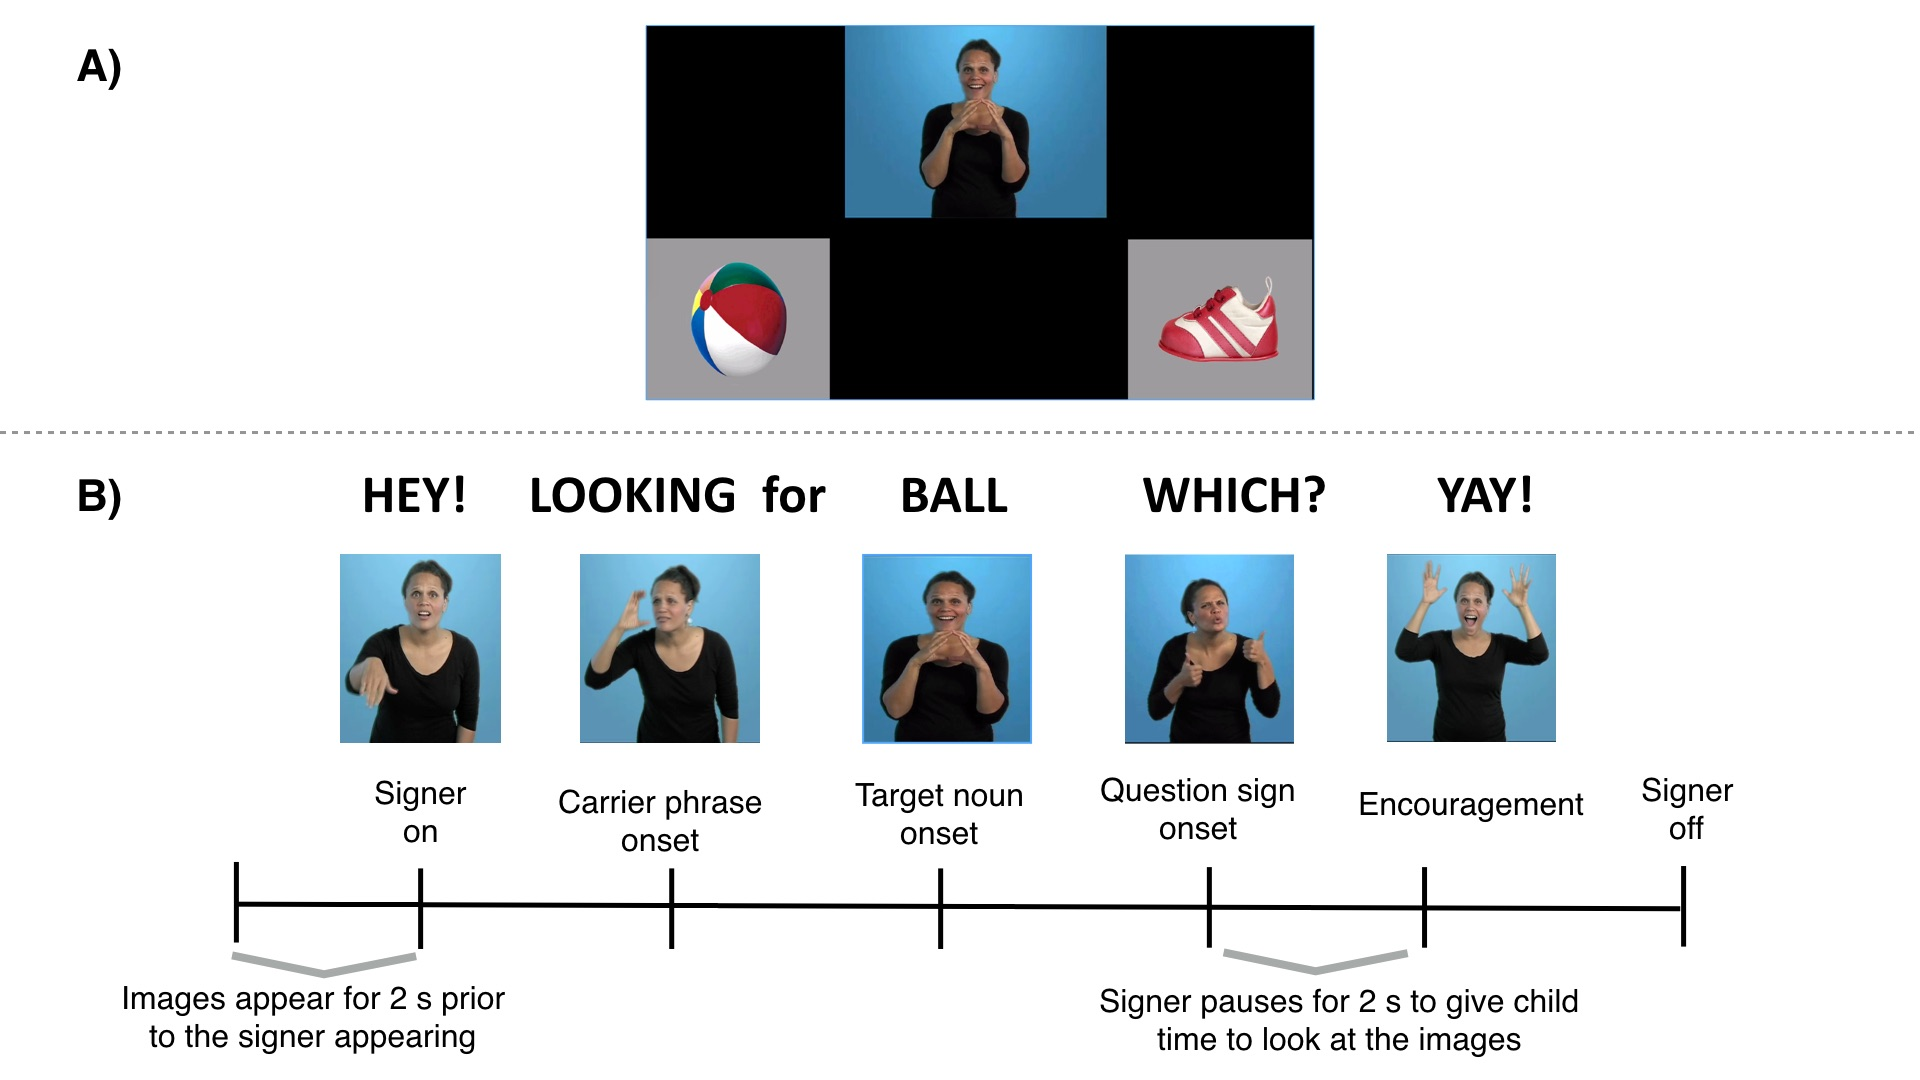
\includegraphics[width=0.95\linewidth]{/Users/ejyoon/Documents/Documents/Research/dissertation/index/chapter_child_rmds/SOL/figures/figure1} 

}

\caption[Stimuli in the Visual Language Processing Task used in Experiment 1.1]{Configuration of visual stimuli (1A) and trial structure (1B) for one question type (sentence final wh-phrase) shown in the central video on the VLP task.}\label{fig:sol-trial-fig}
\end{figure}
\subsubsection{Trial Structure}\label{trial-structure}

Figure 1 shows the structure of a trial with a sentence-final wh-phrase,
one of the two question types in the VLP task. On each trial, children
saw two images of familiar objects on the screen for 2 s before the
signer appeared, allowing time for children to inspect both images.
Next, children saw a still frame of the signer for one second, so they
could orient to the signer prior to sentence onset. The target sentence
was then presented, followed by a question and 2-s hold, followed by an
exclamation to encourage attention to the task. This structure is nearly
identical to the auditory LWL task, differing only in the addition of
the 2-s hold. The hold was included to give participants additional time
to shift gaze from the signer to the objects.

\subsubsection{Calculating measures of language processing
efficiency}\label{calculating-measures-of-language-processing-efficiency}

\emph{Computing target sign onset and offset.} In studies of spoken
language processing, target word onset is typically identified as the
first moment in the auditory signal when there is acoustic evidence of
the target word. However, in signed languages like ASL, phonological
information is present in several components of the visual signal
simultaneously -- for example, in one or both hands as well as in the
face of the signer - making it difficult to determine precisely the
beginning of the target sign. Because sign onset is critical to
operationalizing speed of ASL comprehension in this task, we applied an
empirical approach to defining target-sign onset. We used a gating task
in which adult signers viewed short videos of randomly presented tokens
that varied in length. Two native signers first selected a sequence of
six candidate frames for each token, and then 10 fluent adult signers
unfamiliar with the stimuli watched videos of the target signs in
real-time while viewing the same picture pairs as in the VLP task.
Participants indicated their response with a button press. For each sign
token, the onset of the target noun was operationalized as the earliest
video frame? at which adults selected the correct picture with 100\%
agreement. To determine sign offset, two native signers independently
marked the final frame at which the handshape of each target sign was no
longer identifiable. Agreements were resolved by discussion. Sign length
was defined as sign offset minus sign onset (Median sign length was 1204
ms, ranging from 693-1980 ms).

\emph{Reaction Time.} Reaction time (RT) corresponds to the latency to
shift from the central signer to the target picture on all
signer-to-target shifts, measured from target-noun onset. We chose
cutoffs for the window of relevant responses based on the distribution
of children's RTs in the VLP task, including the middle 90\% (600-2500
ms) (see Ratcliff, 1993). Incorrect shifts (signer-to-distracter
{[}19\%{]}, signer-to-away {[}14\%{]}, no shift {[}8\%{]}) were not
included in the computation of median RT. The RT measure was reliable
within participants (Cronbach's \(\alpha = 0.8\)).

\emph{Target Accuracy.} Accuracy was the mean proportion of time spent
looking at the target picture out of the total time looking at either
target or distracter picture over the 600 to 2500 ms window from target
noun onset. We chose this window to be consistent with the choice of the
RT analysis window. This measure of accuracy reflects the tendency both
to shift quickly from the signer to the target picture in response to
the target sign and to maintain fixation on the target picture. Mean
proportion looking to target was calculated for each participant for all
trials on which the participant was fixating on the center image at
target-sign onset. To make accuracy proportion scores more suitable for
modeling on a linear scale, all analyses were based on scores that were
scaled in log space using a logistic transformation. The Accuracy
measure was reliable within participants (Cronbach's \(\alpha = 0.92\))

\emph{Proportion Sign Length Processed Prior to Shifting.} As a measure
of incremental processing, we used the mean proportion of the target
sign that children and adults saw before generating an initial eye
movement away from the central signer. Because target signs differed in
length across trials, we divided each RT value by the length of the
corresponding target sign. Previous research on spoken language suggests
that at least 200 ms is required to program an eye-movement (Salverda,
Kleinschmidt, \& Tanenhaus, 2014), so we subtracted 200 ms from each RT
to account for eye movements that were initiated during the end of the
target sign (proportion target sign =
\(\frac{(RT-200 \text{ms})}{\text{Sign Length}}\)). Mean proportion of
sign processed was computed for each token of each target sign and then
averaged over all target signs within participants, reflecting the
amount of information signers processed before generating an eye
movement, on average. A score of \(\geq\) 1.0 indicates that a signer
tended to initiate eye movements to the target pictures after sign
offset. An average \(<\) 1.0 indicates eye-movements were planned during
the target sign, reflecting the degree to which signers showed evidence
of incremental language processing.

\subsection{Analysis Plan}\label{analysis-plan}

We used Bayesian methods to estimate the associations between hearing
status, age, vocabulary, and RT and accuracy in the VLP task. Bayesian
methods are desirable for two reasons: First, Bayesian methods allowed
us to quantify support in favor of a null hypothesis of interest -- in
this case, the absence of a difference in real-time processing skills
between age-matched deaf and hearing ASL learners. Second, since native
ASL learners are rare, we wanted to use a statistical approach that
allowed us to incorporate relevant prior knowledge to constrain our
estimates of the strength of association between RT/accuracy on the VLP
task and age/vocabulary.

Concretely, we used prior work on the development of real-time
processing efficiency in children learning spoken language (Fernald et
al., 2008) to consider only plausible linear associations between
age/vocabulary and RT/accuracy, thus making our alternative hypotheses
more precise. In studies with adults, the common use of eye movements as
a processing measure is based on the assumption that the timing of the
first shift reflects the speed of their word recognition (Tanenhaus,
Magnuson, Dahan, \& Chambers, 2000).\footnote{The assumption that first
  shifts reflects speed of incremental word recognition depends on the
  visual display containing candidate objects with minimal initial
  phonological overlap. If there are phonological competitors present
  (e.g., candy vs.~candle), then participants' early shifting behavior
  could reflect consideration of alternative lexical hypotheses for the
  incoming linguistic information.} However, studies with children have
shown that early shifts are more likely to be random than later shifts
(Fernald et al., 2008), suggesting that some children's shifting
behavior may be unrelated to real-time ASL comprehension. We use a
mixture-model to quantify the probability that each child participant's
response is unrelated to their real-time sign recognition (i.e., that
the participant is responding randomly, or is ``guessing''), creating an
analysis model where participants who were more likely to be guessers
have less influence on the estimated relations between RT and
age/vocabulary. Note that we use this approach only in the analysis of
RT, since ``guessing behavior'' is integral to our measure of children's
mean accuracy in the VLP task, but not to our measure of mean RT. The
Supplemental Material available online provides more details about the
analysis model, as well two additional sensitivity analyses, which
provide evidence that our results are robust to different specifications
of prior distributions and to different analysis windows. We also
provide a parallel set of analyses using a non-Bayesian approach, which
resulted in comparable findings.

To provide evidence of developmental change, we report the strength of
evidence for a linear model with an intercept and slope, compared to an
intercept-only model in the form of a Bayes Factor (BF) computed via the
Savage-Dickey method (Wagenmakers et al., 2010). To estimate the
uncertainty around our estimates of the linear associations, we report
the 95\% Highest Density Interval (HDI) of the posterior distribution of
the intercept and slope. The HDI provides a range of plausible values
and gives information about the uncertainty of our point estimate of the
linear association. Models with categorical predictors were implemented
in STAN (Stan Development Team, 2016), and models with continuous
predictors were implemented in JAGS (Plummer, 2003). Finally, we chose
the linear model because it a simple model of developmental change with
only two parameters to estimate, and the outcome measures -- mean RT and
Accuracy for each participant -- were normally distributed. All of the
linear regressions include only children's data and take the form:
\(\textit{processing measure ~ age}\) and
\(\textit{processing measure ~ vocabulary}\).

\subsection{Results}\label{results}

The results are presented in five sections addressing the following
central questions in this research. First, where do ASL users look while
processing sign language in real-time? Here we provide an overview of
the time course of looking behavior in our task for both adults and
children. Second, would young ASL-learners and adult signers show
evidence of rapid gaze shifts that reflect lexical processing, despite
the apparent competition for visual attention between the language
source and the nonlinguistic visual world? In this section, we estimate
the degree to which children and adults tended to initiate eye-movements
prior to target sign offset, providing evidence that these gaze shifts
occur prior to sign offset and index speed of incremental ASL
comprehension. Third, do deaf and hearing native signers show a similar
time course of eye movements, despite having differential access to
auditory information in their daily lives? Or would deaf children's
daily experience relying on vision to monitor both the linguistic signal
and the potential referents in the visual world result in a
qualitatively different pattern of performance, e.g., their waiting
longer to disengage from the signer to seek the named object? Fourth, do
young ASL-learners show age-related increases in processing efficiency
that parallel those found in spoken languages? Here we compare
ASL-learners' processing skills to those of adult signers and exploring
relations to age among the children. Finally, is individual variation in
children's ASL processing efficiency related to the size of their
productive ASL vocabularies?
\begin{figure}[t]

{\centering 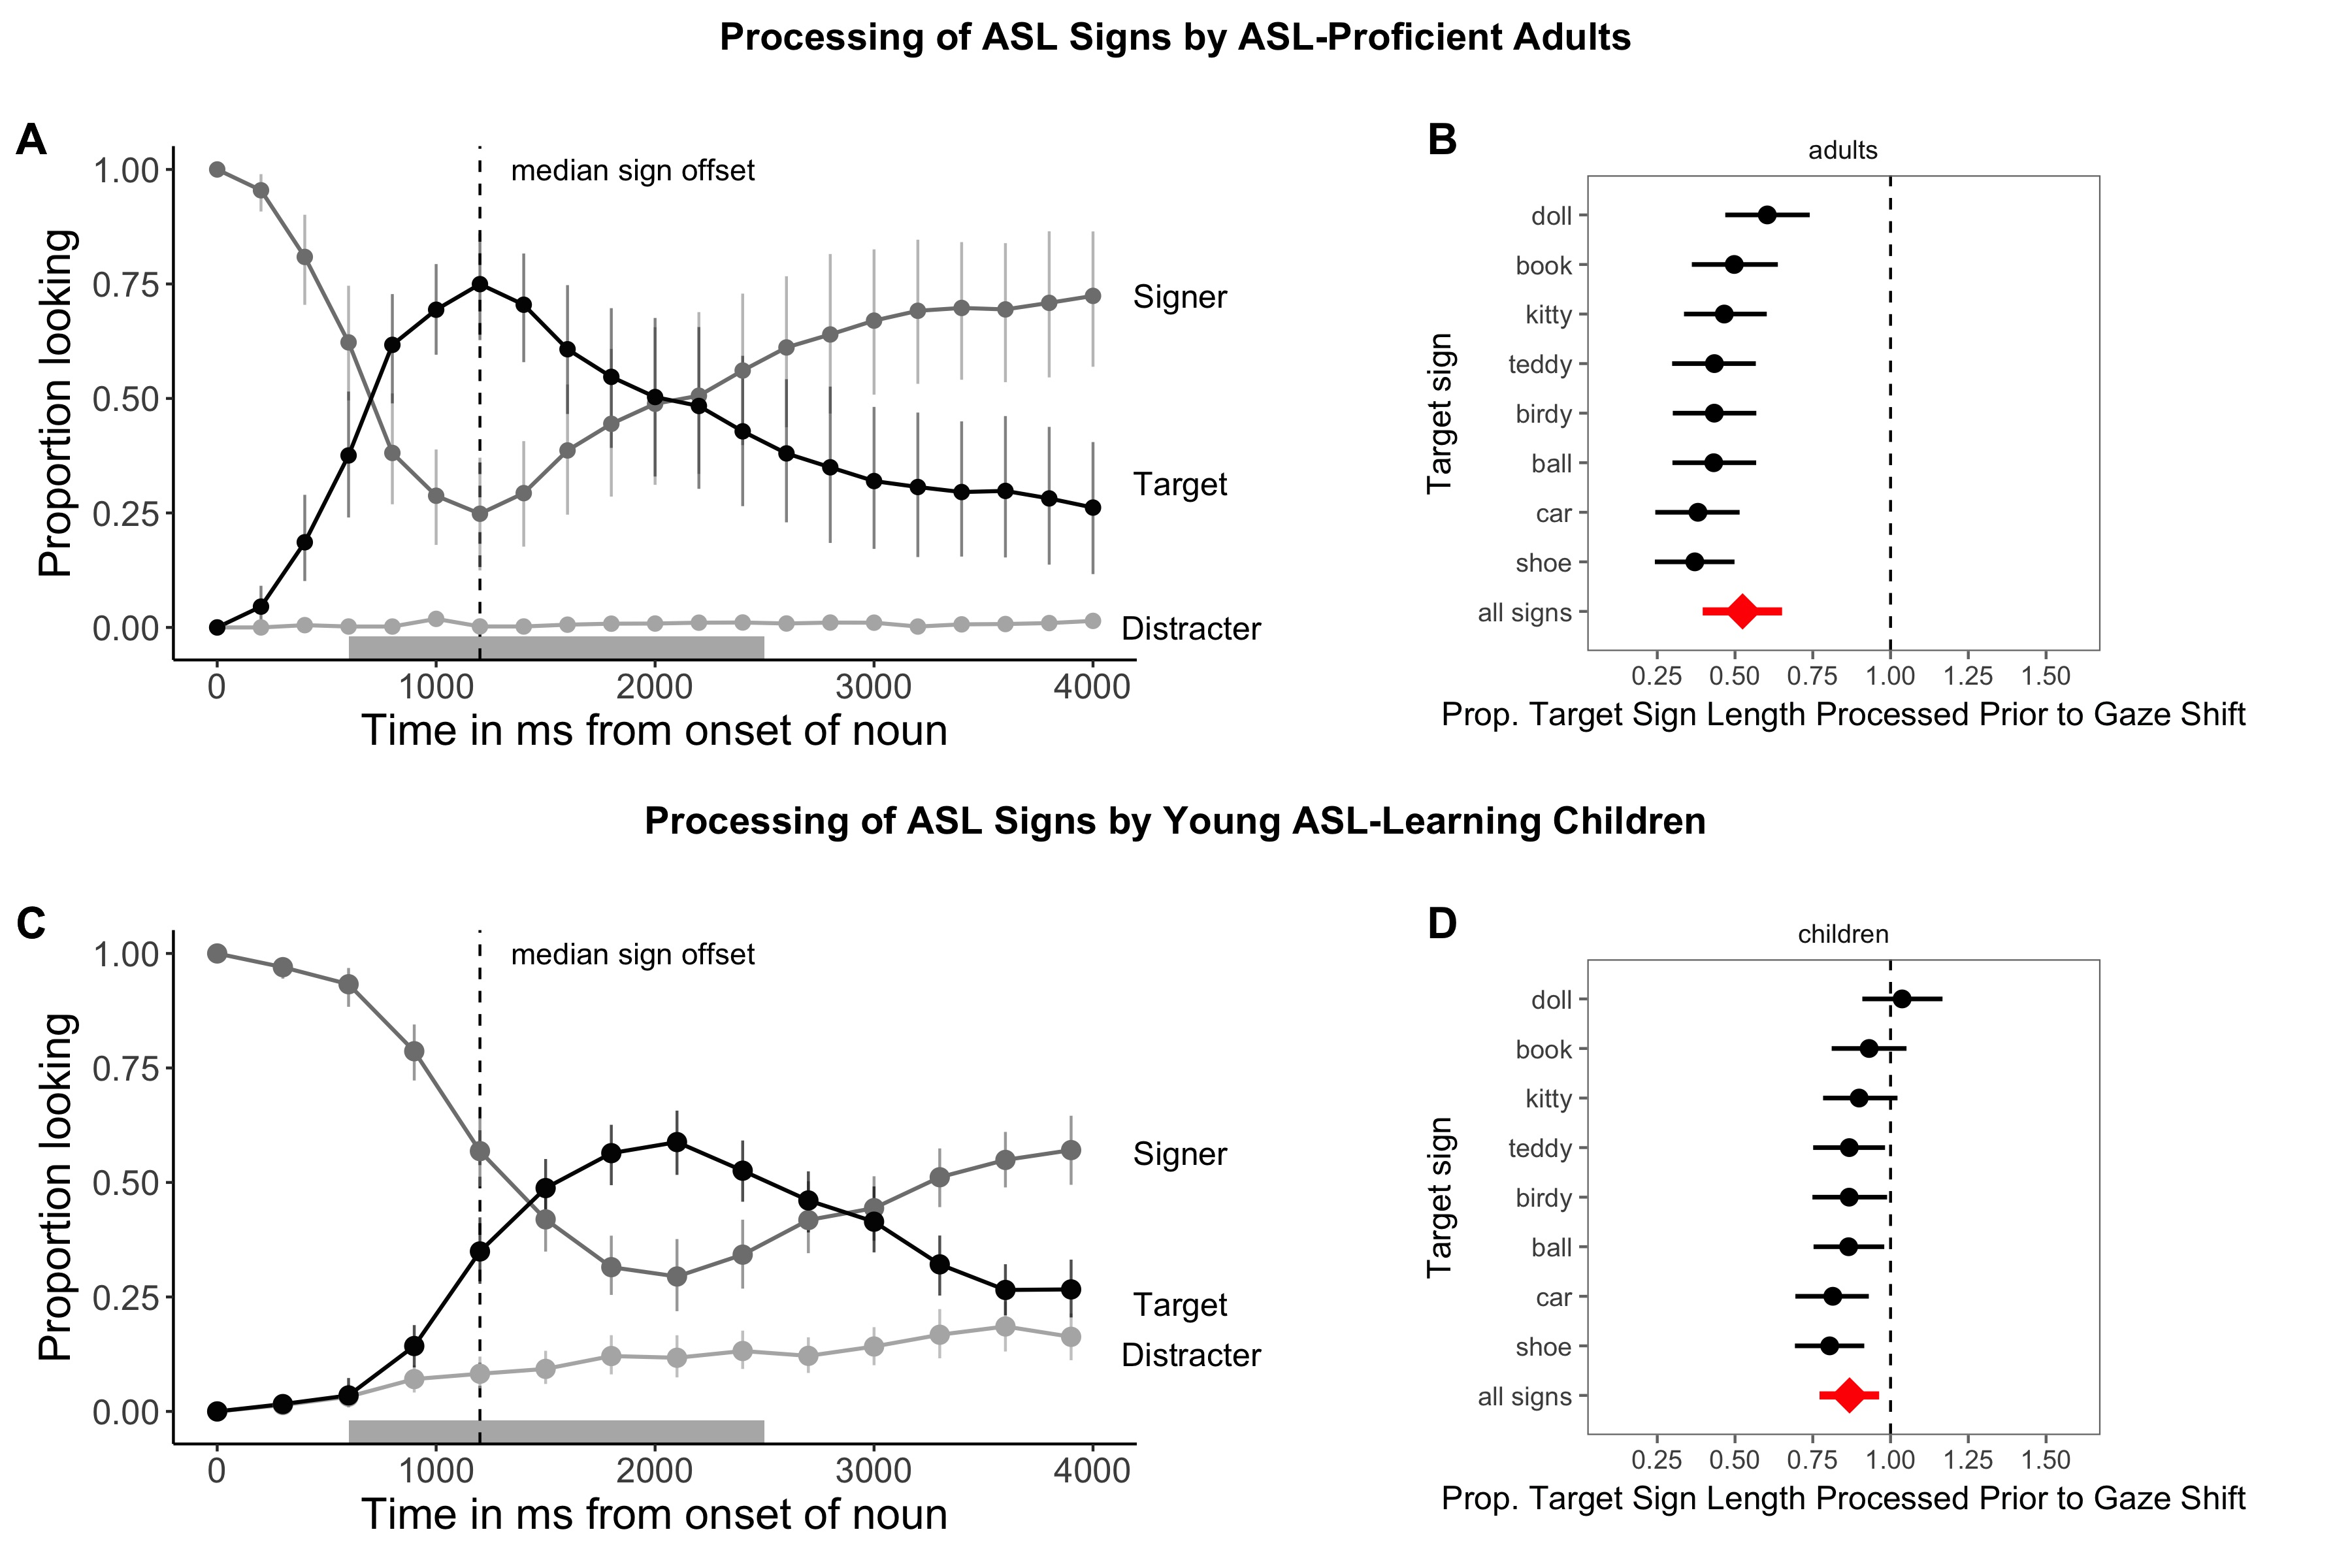
\includegraphics[width=0.95\linewidth]{/Users/ejyoon/Documents/Documents/Research/dissertation/index/chapter_child_rmds/SOL/figures/figure2} 

}

\caption[Time course looking behavior for ASL-proficient adults and young ASL-learners]{The time course of looking behavior for ASL-proficient adults (2A) and young ASL-learners (2C). The curves show mean proportion looking to the signer (dark grey), the target image (black), and the distracter image (light grey). The grey shaded region marks the analysis window (600-2500ms); error bars represent +/- 95\% CI computed by non-parametric bootstrap. The mean proportion of each target sign length (see the Methods section for details on how sign length was defined) processed prior to shifting visual attention away from the language source to a named object for adults (2B) and children (2D). The diamond indicates the mean estimate for all signs. The dashed vertical line corresponds to a median proportion of 1.0. Error bars represent 95\% Highest Density Intervals.}\label{fig:sol-tc-figure}
\end{figure}
\subsubsection{Overview of looking behavior during real-time ASL
comprehension}\label{overview-of-looking-behavior-during-real-time-asl-comprehension}

The first question of interest was where do ASL users look while
processing sign language in real-time? Figure 2 presents an overview of
adults (2A) and children's (2B) looking behavior in the VLP task. This
plot shows changes in the mean proportion of trials on which
participants fixated the signer, the target image, or the distracter
image at every 33-ms interval of the stimulus sentence. At target-sign
onset, all participants were looking at the signer on all trials. As the
target sign unfolded, the mean proportion looking to the signer
decreased rapidly as participants shifted their gaze to the target or
the distracter image. Proportion looking to the target increased sooner
and reached a higher asymptote, compared to proportion looking to the
distracter, for both adults and children. After looking to the target
image, participants tended to shift their gaze rapidly back to the
signer, shown by the increase in proportion looking to the signer around
2000 ms after target-noun onset. Adults tended to shift to the target
picture sooner in the sentence than did children, and well before the
average offset of the target sign. Moreover, adults rarely looked to the
distractor image at any point in the trial. This systematic pattern of
behavior -- participants reliably shifting attention from the signer to
the named object and back to the signer -- provides qualitative evidence
that the VLP task is able to capture interpretable eye movement behavior
during ASL comprehension.

\subsubsection{Evidence that eye movements during ASL processing index
incremental sign
comprehension}\label{evidence-that-eye-movements-during-asl-processing-index-incremental-sign-comprehension}

One of the behavioral signatures of proficient spoken language
processing is the rapid influence of language on visual attention, with
eye movements occurring soon after listeners have enough information to
identify the named object. Our second question of interest was whether
young ASL-learners and adult signers would also show evidence of rapid
gaze shifts in response to signed language, despite the apparent
competition for visual attention between the language source and the
nonlinguistic visual world. Or would signers delay their shifts until
the very end of the target sign, or even until the end of the utterance,
perhaps because they did not want to miss subsequent linguistic
information?

To answer these questions, we conducted an exploratory analysis,
computing the proportion of each target sign that participants processed
before generating an eye movement to the named object. Figure 2 shows
this measure for each target sign for both adults (2B) and children
(2D). Adults shifted prior to the offset of the target sign for all
items and processed on average 51\% of the target sign before generating
a response (M = 0.51, 95\% HDI {[}0.35, 0.66{]}). Children processed
88\% of the target sign on average, requiring more information before
shifting their gaze compared to adults. Children reliably initiated
saccades prior to the offset of the target sign overall (M = 0.88, 95\%
HDI {[}0.79, 0.98{]}) and for five out of the eight signed stimuli.

These results suggest that young signers as well as adults process signs
incrementally as they unfold in time (for converging evidence see
Lieberman et al., 2015, 2017). It is important to point out that we
would not interpret signers waiting until the end of the sign or the end
of the sentence as evidence against an incremental processing account
since there could be other explanations for that pattern of results such
as social norms of looking at a person until they finish speaking.
However, this result provides positive evidence that eye movements in
the VLP task provide an index of speed of incremental ASL comprehension,
allowing us to perform the subsequent analyses that estimate (a) group
differences in looking behavior and (b) links between individual
variation in speed and accuracy of eye movements during ASL processing
and variation in productive vocabulary.
\begin{figure}[t]

{\centering 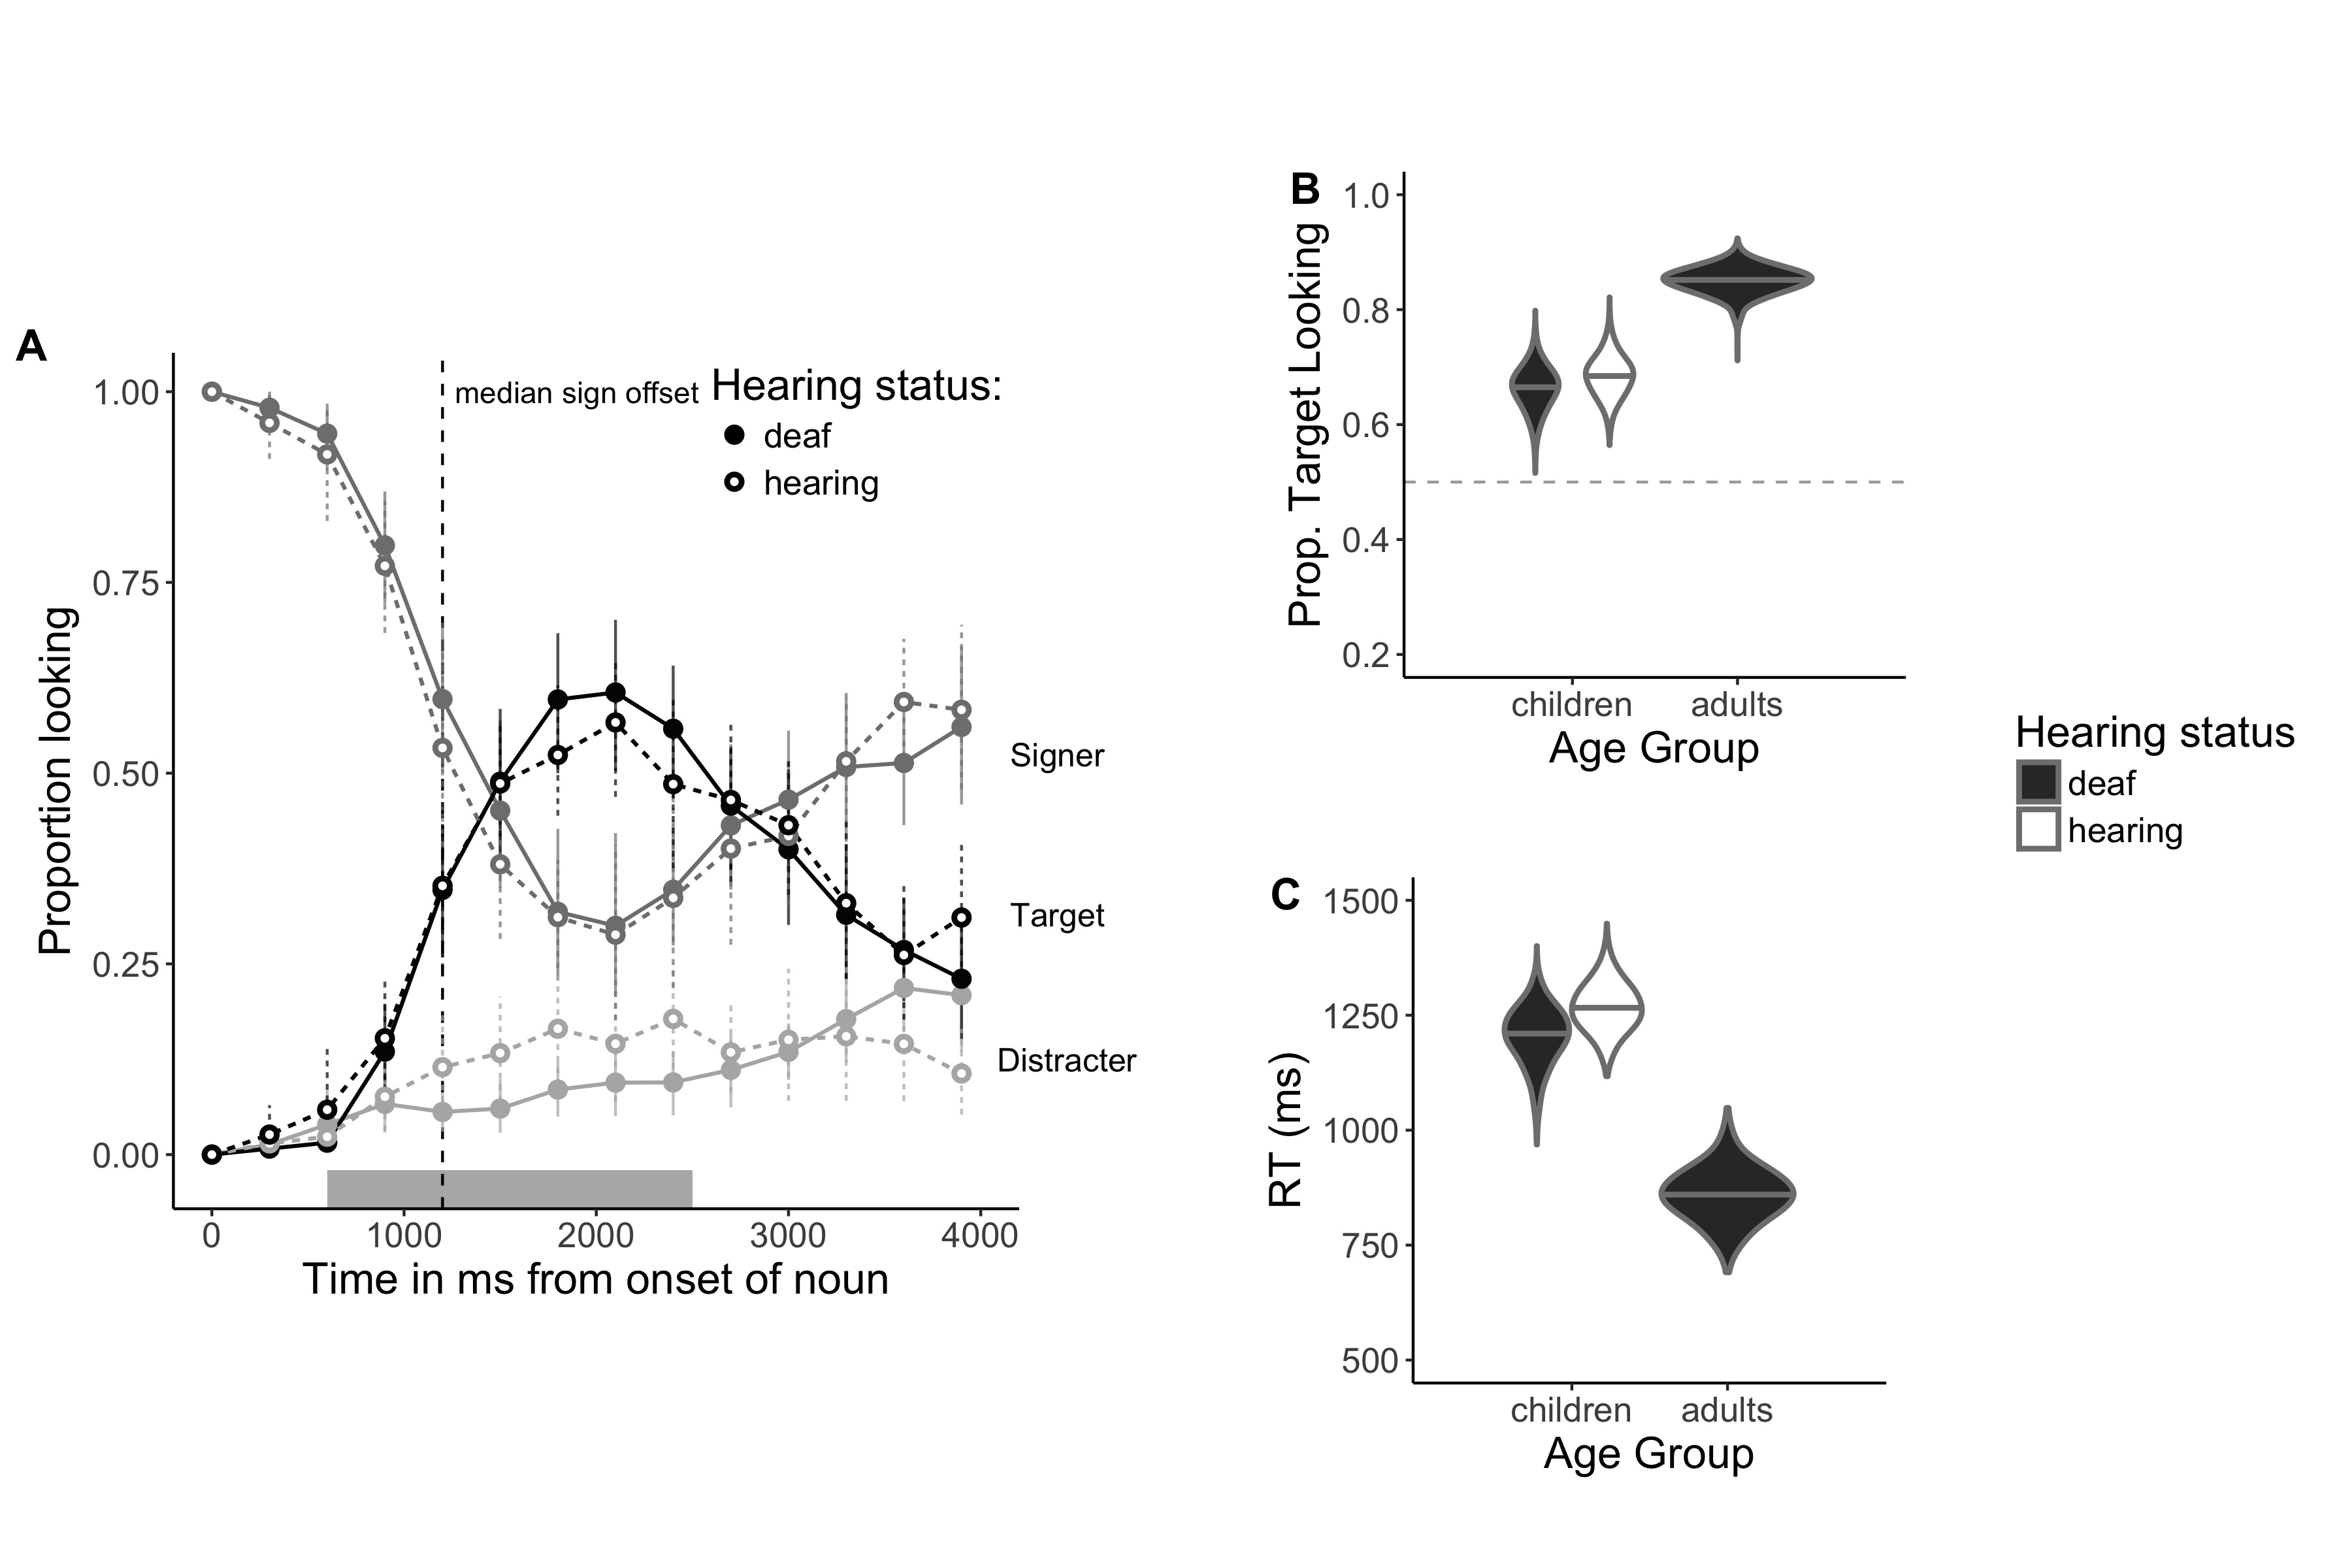
\includegraphics[width=0.95\linewidth]{/Users/ejyoon/Documents/Documents/Research/dissertation/index/chapter_child_rmds/SOL/figures/figure3} 

}

\caption[The time course of looking behavior for young deaf and hearing ASL-learners]{The time course of looking behavior for young deaf and hearing ASL-learners (3A). Filled circles represent deaf signers, while open circles represent hearing signers; All other plotting conventions are the same as in Figure 2. Panels B and C show full posterior distributions over model estimates for mean Accuracy (3B) and Reaction Time (3C) for children and adults. Fill (white/black) represents children's hearing status. (Note that there were no hearing adult signers in our sample).}\label{fig:sol-tc-coda-figure}
\end{figure}
\subsubsection{Real-time ASL comprehension in deaf and hearing children
and deaf
adults}\label{real-time-asl-comprehension-in-deaf-and-hearing-children-and-deaf-adults}

The third question of interest was whether deaf and hearing native
signers show a similar time course of lexical processing, driven by
their similar language experiences and the in-the-moment constraints of
interpreting a sign language in real time? Or would deaf children's
daily experience relying on vision to monitor both the linguistic signal
and the potential referents in the visual world result in a
qualitatively different pattern of performance, e.g., their waiting
longer to disengage from the signer to seek the named object?

Figure 3A presents the overview of looking behavior for deaf and hearing
children. At target-sign onset, all children were looking at the signer
on all trials. Overall, deaf and hearing children showed a remarkably
similar time course of looking behavior: shifting away from the signer,
increasing looks to the target, and shifting back to the signer at
similar time points as the sign unfolded. To quantify any differences,
we compared the posterior distributions for mean accuracy (Figure 3B)
and mean RT (Figure 3C) across the deaf and hearing groups. We did not
find evidence for a difference in mean accuracy (\(M_{hearing} = 0.68\),
\(M_{deaf} = 0.65\); \(\beta_{diff} = 0.03\), 95\% HDI
\([-0.07, 0.13]\)) or RT (\(M_{hearing} = 1265.62\) ms,
\(M_{deaf} = 1185.05\) ms; \(\beta_{diff} = 78.32\) ms, 95\% HDI
\([-86.01 ms, 247.04 ms]\)), with the 95\% HDI including zero for both
models. These parallel results provide evidence that same-aged hearing
and deaf native ASL-learners showed qualitatively similar looking
behavior during real-time sentence processing, suggesting that decisions
about where to allocate visual attention are not modulated by
differential access to auditory information, but rather are shaped by
learning ASL as a first language (see Bavelier et al., 2006 for a review
of the differential effects of deafness compared to learning a visual
language on perception and higher-order cognitive skills). Moreover,
these results provide additional justification (over and above
children's highly similar language background experience) for analyzing
all the native ASL-learning children together, regardless of hearing
status, in the subsequent analyses.
\begin{figure}[t]

{\centering 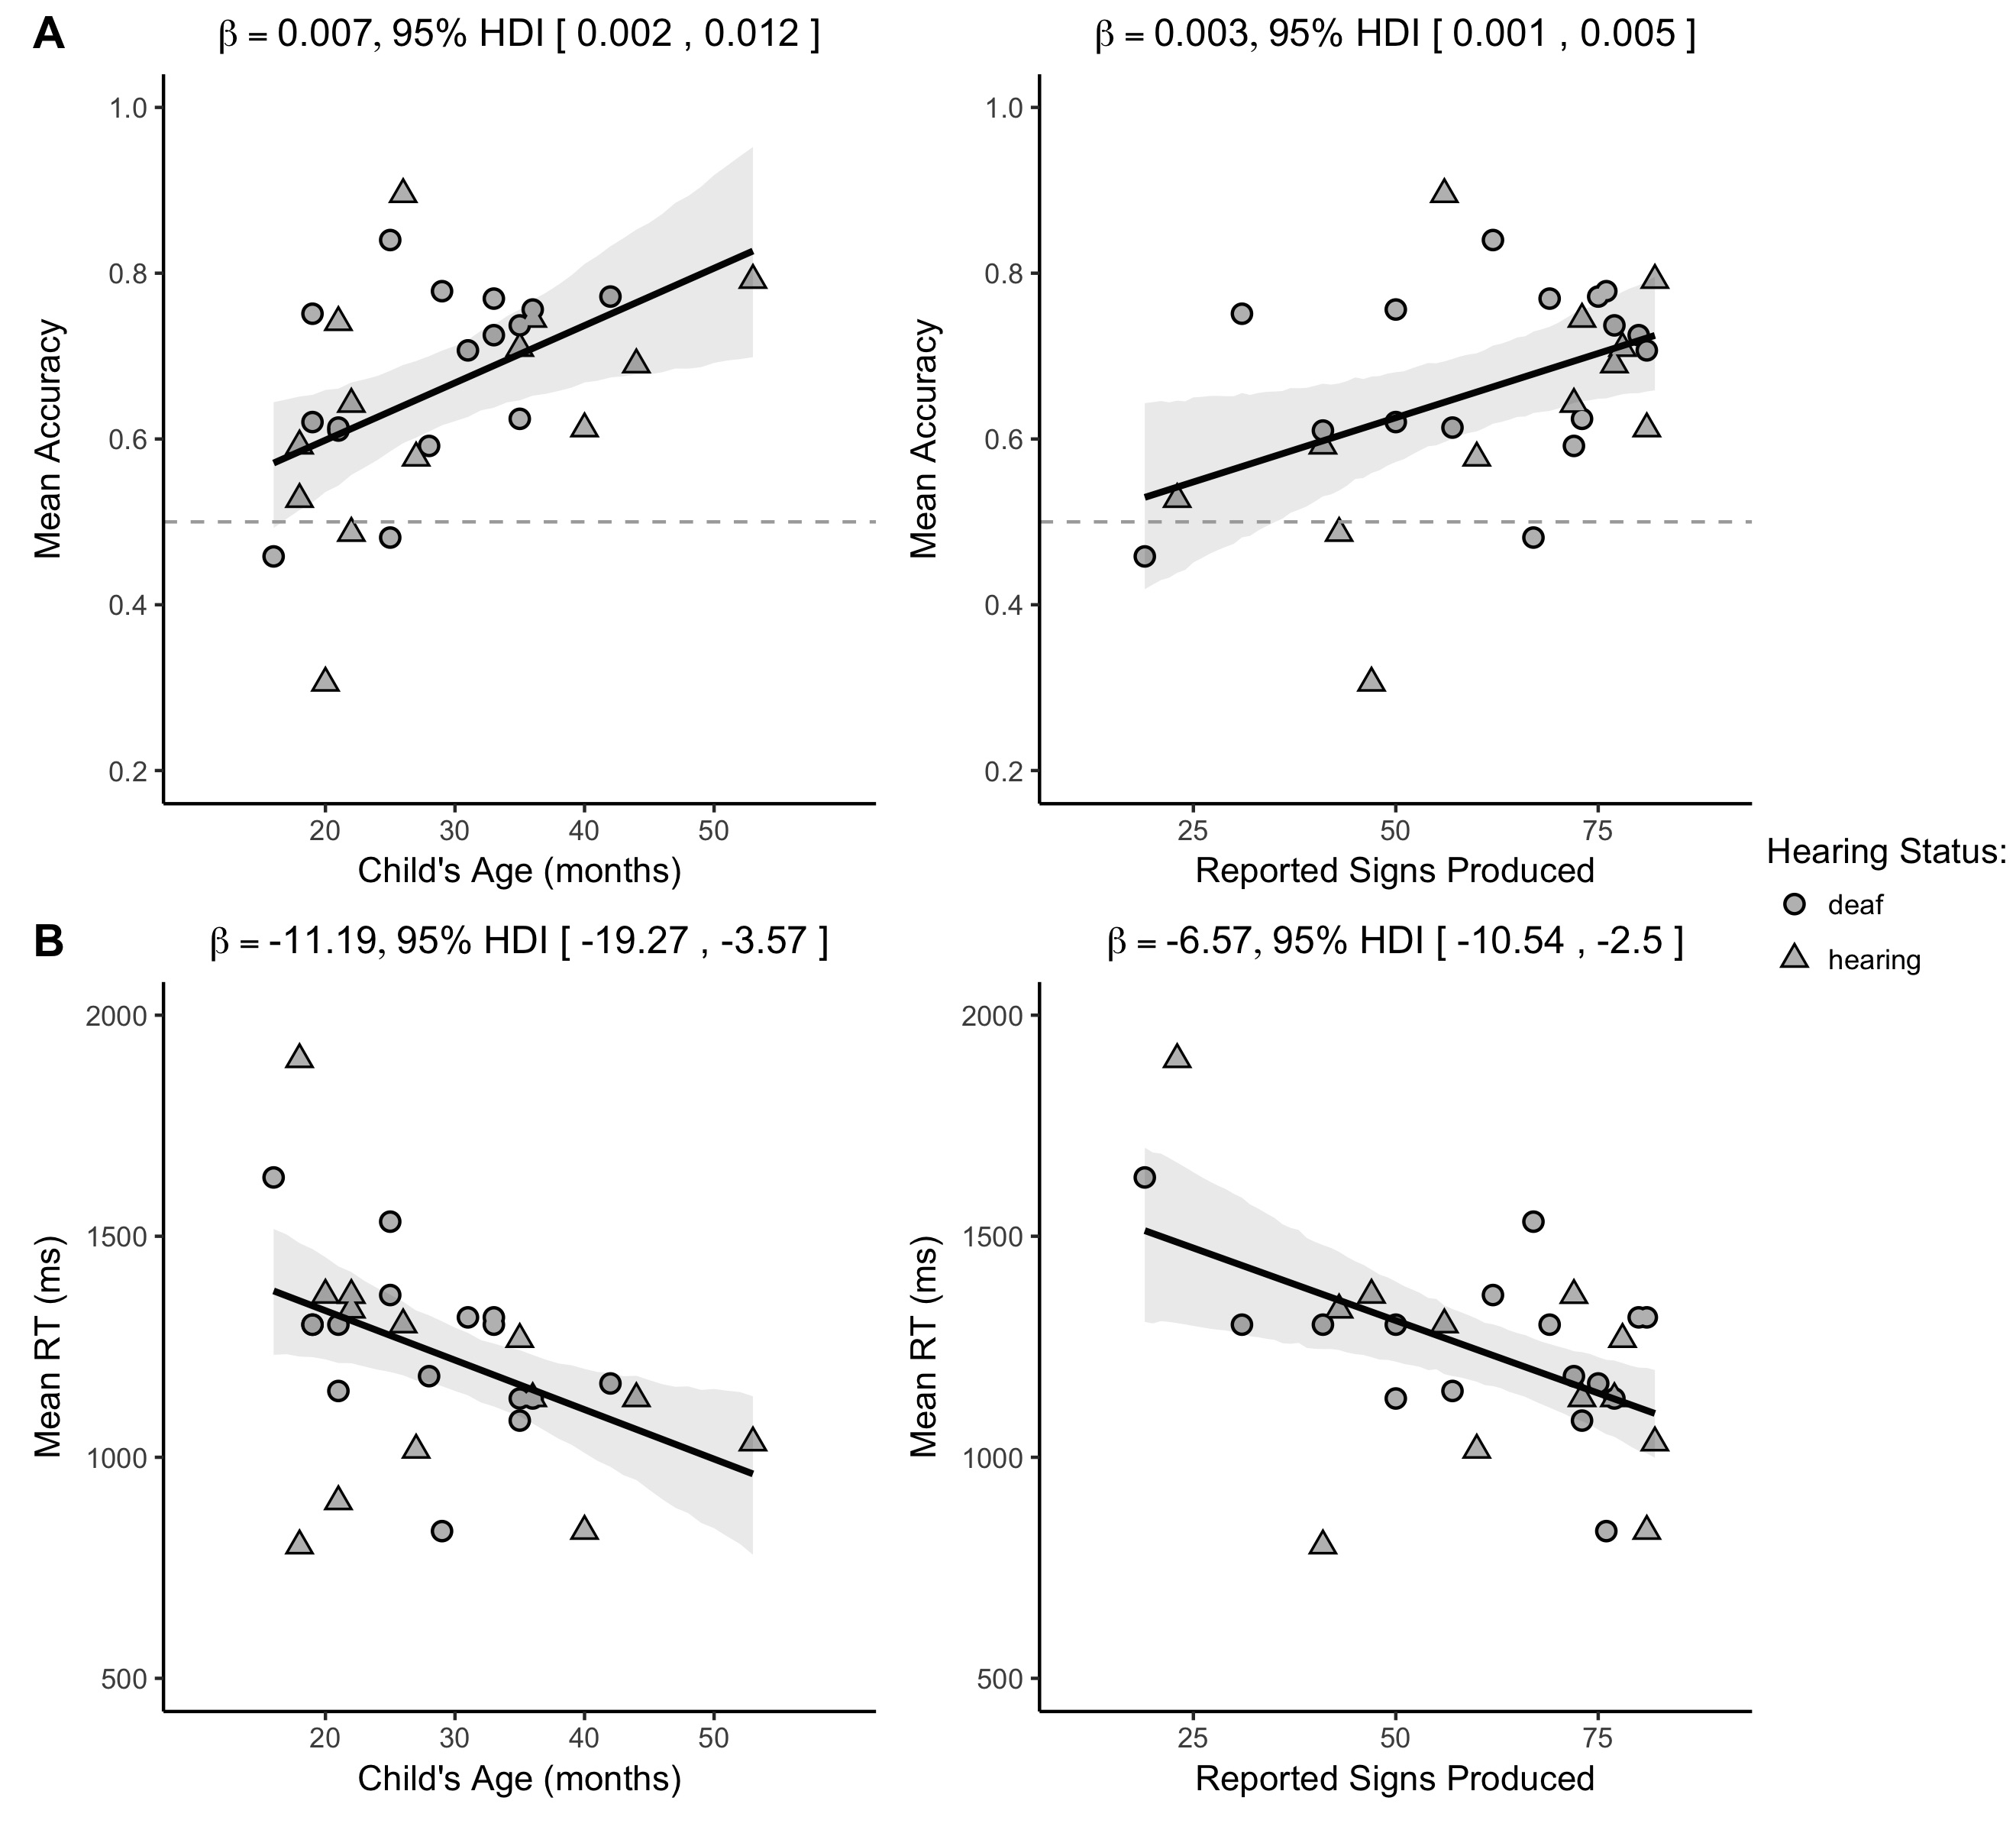
\includegraphics[width=0.8\linewidth]{/Users/ejyoon/Documents/Documents/Research/dissertation/index/chapter_child_rmds/SOL/figures/figure4} 

}

\caption[Scatterplots of relations between children's age and vocabulary and ASL processing]{Scatterplots of relations between children's age and vocabulary and measures of their mean accuracy (4A) and mean RT (4B) in the VLP procedure. Shape represents children's hearing status. The solid black line is the maximum a posteriori model estimate for the mean accuracy at each age point. The shaded gray regions represent the 95\% Highest Density Interval (range of plausible values) around the regression line.}\label{fig:sol-corr-figure}
\end{figure}
Next, we compared real-time processing efficiency in ASL-learners and
adult signers. Returning to the overview of looking behavior shown in
Figure 2, we see that adults tended to shift to the target picture
sooner in the sentence than did children, and well before the average
offset of the target sign. Moreover, adults rarely looked to the
distractor image at any point in the trial. To quantify these
differences we computed the full posterior distribution for children and
adults' mean Accuracy (Figure 3B) and RT (Figure 3C). Overall, adults
were more accurate (\(M_{adults}= 0.85\), \(M_{children} = 0.68\),
\(\beta_{diff} = 0.17\), 95\% HDI for the difference in means {[}0.11,
0.24{]}) and faster to shift to the target image compared to children
(\(M_{adults}= 861.98\) ms, \(M_{children} = 1229.95\) ms;
\(\beta_{diff} = -367.76\) ms, 95\% HDI for the difference in means
{[}-503.42 ms, -223.85 ms{]}). This age-related difference parallels
findings in spoken language (Fernald et. al., 2006) and shows that young
ASL learners are still making progress towards adult-levels of ASL
processing efficiency.

\subsubsection{Links between children's age and efficiency in
incremental sign
comprehension}\label{links-between-childrens-age-and-efficiency-in-incremental-sign-comprehension}

The fourth question of interest was whether young ASL-learners show
age-related increases in processing efficiency that parallel those found
in spoken languages. To answer this question, we estimated relations
between young ASL learners' age-related increases in the speed and
accuracy with which they interpreted familiar signs (see Table 3 for
point and interval estimates). Mean accuracy was positively associated
with age (Figure 4A), indicating that older ASL learners were more
accurate than younger children in fixating the target picture. The Bayes
Factor (BF) indicated that a model including a linear association was
12.8 times more likely than an intercept-only model, providing strong
evidence for developmental change. The \(\beta\) estimate indicates
that, for each month of age, children increased their accuracy score by
0.007, i.e., an increase of \textasciitilde{}1\% point, meaning that
over the course of one year the model estimates a \textasciitilde{}12\%
point gain in accuracy when establishing reference in the VLP task. Mean
RTs were negatively associated with age (Figure 4A), indicating that
older children shifted to the target picture more quickly than did
younger children. The BF was \textasciitilde{}14, providing strong
evidence for a linear association. The model estimates a
\textasciitilde{}11 ms gain in RT for each month, leading to a
\textasciitilde{}132 ms gain in speed of incremental ASL comprehension
over one year of development.

Together, the accuracy and RT analyses showed that young ASL learners
reliably looked away from the central signer to shift to the named
target image in the VLP task. Importantly, children varied in their
response times and accuracy, and this variation was meaningfully linked
to age. Thus, like children learning spoken language, ASL learners
improve their real-time language processing skills over the second and
third years of life as they make progress towards adult levels of
language fluency.
\begin{longtable}[t]{>{\raggedright\arraybackslash}p{4cm}rll}
\caption[Summary of the four linear models using children's age and vocabulary size to predict accuracy and reaction time]{\label{tab:sol-bf-table}Summary of the four linear models using children's age and vocabulary size to predict accuracy (proportion looking to target) and reaction time (latency to first shift in ms). BF is the Bayes Factor comparing the evidence in favor of linear model to an intercept-only (null) model; Mean Beta is the mean of the posterior distribution for the slope parameter for each model (i.e., the linear association); and the Highest Density Interval (HDI) shows the interval containing 95\% of the plausible slope values given the model and the data.}\\
\toprule
\textbf{Model specification} & \textbf{Bayes Factor} & \textbf{Mean Beta} & \textbf{95\% HDI}\\
\midrule
Accuracy \textasciitilde{} Age & 12.8 & 0.007 & [0.002, 0.012]\\
Accuracy \textasciitilde{} Vocab & 6.8 & 0.003 & [0.001, 0.005]\\
RT \textasciitilde{} Age & 14.4 & -11.2 ms & [-19.3 ms, -3.6 ms]\\
RT \textasciitilde{} Vocab & 18.7 & -6.6 ms & [-10.5 ms, -2.5 ms]\\
\bottomrule
\end{longtable}
\subsubsection{Links between children's incremental sign comprehension
and productive
vocabulary}\label{links-between-childrens-incremental-sign-comprehension-and-productive-vocabulary}

The final question of interest was whether individual differences in
processing skills were related to the size of children's ASL
vocabularies. As shown in Figure 4B, children with higher accuracy
scores also had larger productive vocabularies (BF = 6.8), with the
model estimating a 0.003 increase for each additional sign known.
Moreover, children who were faster to recognize ASL signs were those
with larger sign vocabularies (BF = 18.7), with each additional sign
resulting in a \textasciitilde{}7 ms decrease in estimated RT. Taken
together, older children and children with larger expressive
vocabularies were more accurate and efficient in identifying the
referents of familiar signs. It is important to point out that the
independent effect of vocabulary size on ASL processing could not be
assessed here given the correlation between age and vocabulary (r =
0.76) in our sample of children ages one to four years. However, these
findings parallel results in the substantial body of previous research
with monolingual children learning spoken languages, such as English
(Fernald et al., 2006) and Spanish (Hurtado, Marchman, \& Fernald,
2007).

\section{Discussion}\label{discussion}

Efficiency in establishing reference in real-time lexical processing is
a fundamental component of language learning. Here, we developed the
first measures of young ASL learners' real-time language comprehension
skills. There are five main findings from this research.

First, both adults and children showed a similar qualitative pattern of
looking behavior as signs unfolded in time. They began by looking at the
signer to gather information about the signed sentence, before shifting
gaze to the named object, followed by a return in looking to the signer.
All signers allocated very few fixations to the distractor image at any
point during the signed sentence.

Second, children and adults tended to shift their gaze away from the
signer and to the named referent prior to sign offset, providing
evidence of incremental ASL processing. This rapid influence of language
on visual attention in ASL is perhaps even more striking since premature
gaze shifts could result in a degraded the linguistic signal processed
in the periphery or in missing subsequent linguistic information
altogether. Furthermore, evidence of incremental gaze shifts suggests
that eye movements during ASL processing index efficiency of lexical
comprehension, as previously shown in spoken languages, which is
important for future work on the psycholinguistics of early sign
language acquisition.

Third, deaf and hearing native signers, despite having differential
access to auditory information, showed remarkably similar looking
behavior during real-time ASL comprehension. Even though the deaf and
hearing children had differential access to auditory information in
their daily lives, this experience did not change their overall looking
behavior or the timing of their gaze shifts during ASL comprehension.
Instead, both groups showed parallel sensitivity to the in-the-moment
constraints of processing ASL in real time. That is, both deaf and
hearing children allocated similar amounts of visual attention to the
signer, presumably because this was the only fixation point in the
visual scene that also provided information with respect to their goal
of language comprehension. This is in stark contrast to what hearing
children could potentially do in a similar grounded language
comprehension task where a speaker was a potential visual target. In
that case, the hearing listener could choose to look at the speaker or
to look elsewhere, without losing access to the incoming language via
the auditory channel. Thus, they can look while they listen.

Fourth, like children learning spoken language, young ASL-learners were
less efficient than adults in their real-time language processing, but
they showed significant improvement with age over the first four years.
Moreover, although all target signs were familiar to children, older
children identified the named referents more quickly and accurately than
younger children. This result suggests that the real-time comprehension
skills of children who are learning ASL in native contexts follow a
similar developmental path to that of spoken language learners, as has
been shown in previous work on ASL production (Lillo-Martin, 1999;
Mayberry \& Squires, 2006). By developing precise measures of real-time
ASL comprehension, we were able to study children's language skills
earlier in development as compared to other methods.

Fifth, we found a link between ASL processing skills and children's
productive vocabularies. ASL-learning children who knew more signs were
also faster and more accurate to identify the correct referent than
those who were lexically less advanced. These results are consistent
with studies of English- and Spanish-learning children, which find
strong relations between efficiency in online language comprehension and
measures of linguistic achievement (Fernald et al., 2006; Marchman \&
Fernald, 2008).

\subsection{Limitations and open
questions}\label{limitations-and-open-questions}

This study has several limitations. First, while the sample size is
larger than in most previous studies of ASL development, it is still
relatively small compared to many studies of spoken language acquisition
- an unsurprising limitation, given that native ASL-learners are a rare
population. Thus more data are needed to characterize more precisely the
developmental trajectories of sign language processing skills. Second,
testing children within a narrower age range might have revealed
independent effects of vocabulary size on ASL processing, which could
not be assessed here given the correlation between age and vocabulary
size in our broad sample of children from one to four years. To
facilitate replication and extension of our results, we have made all of
our stimuli, data, and analysis code publicly available
(\url{https://github.com/kemacdonald/SOL}).

Third, we did not collect measures of age-related gains in children's
general cognitive abilities. Thus, it is possible that our estimates of
age-related changes in lexical processing are influenced by children's
developing efficiency in other aspects of cognition, e.g., increased
control of visual attention. Work on the development of visual attention
from adolescence to early adulthood shows that different components of
visual attention (the ability to distribute attention across the visual
field, attentional recovery from distraction, and multiple object
processing) develop at different rates (Dye and Bavelier, 2009).
Moreover, work by Elsabbagh et. al., (2013) shows that infants become
more efficient in their ability to disengage from a central stimulus to
attend to a stimulus in the periphery between the ages 7 months and 14
months. However, there is a large body of work showing that features of
language use and structure (e.g., the frequency of a word, a word's
neighborhood density, and the amount of language input a child
experiences) affect the speed and accuracy of eye movements in the
Looking-While-Listening style tasks (see Tanenhaus et al., 2000 for a
review). Thus, while it possible that age-related improvements in
general cognitive abilities are a factor in our results, we think that
the strength of the prior evidence suggests that more efficient gaze
shifts in the VLP task are indexing improvements in the efficiency of
incremental ASL comprehension.

A fourth limitation is that characteristics of our task make it
difficult to directly compare our findings with previous work on ASL
processing by adults. For example, in contrast to prior gating studies
(e.g., Emmorey \& Corina, 1990; Morford \& Carlsen, 2011), our stimuli
consisted of full sentences in a child-directed register, not isolated
signs, and we used a temporal response measure rather than an open-ended
untimed response. However, it is interesting to note that the mean
reaction time of the adults in our task (M = 862 ms) is strikingly close
to the average performance of native adult signers in Lieberman et al.'s
(2015) ``unrelated'' condition (M = 844 ms). In addition, we did not
select stimuli that parametrically varied features of signs that may
influence speed of incremental ASL comprehension, including iconicity
and degree of phonological overlap. However, we were able to use a
recently created database of lexical and phonological properties of 1000
signs (Caselli et. al., 2017) to explore this possibility. We did not
see evidence that iconicity or degree of phonological overlap influenced
speed or accuracy of eye movements in children or adults in our sample
of eight target signs (see Figures S4 and S5 in the online supplement).

We also cannot yet make strong claims about processing in signed
vs.~spoken languages in absolute terms because the VLP task included the
signer as a central fixation, resulting in different task demands
compared to the two-alternative procedure used to study children's
spoken language processing (e.g., Fernald et al. 1998). However, a
direct comparison of the timecourse of eye movements during signed and
spoken language processing is a focus of our ongoing work (MacDonald et
al., 2017). Nevertheless, the current results reveal parallels with
previous findings showing incremental processing during real-time spoken
language comprehension (see Tanenhaus et al., 2000) and sign language
comprehension in adults (Lieberman et al., 2015). Moreover, we
established links between early processing efficiency and measures of
vocabulary in young ASL-learners, suggesting that parallel mechanisms
drive language development, regardless of the language modality.

Finally, our sample is not representative of most children learning ASL
in the United States. Since most deaf children are born to hearing
parents unfamiliar with ASL, many are exposed quite inconsistently to
sign language, if at all. We took care to include only children exposed
to ASL from birth. The development of real-time ASL processing may look
different in children who have inconsistent or late exposure to ASL
(Mayberry, 2007). An important step is to explore how variation in ASL
processing is influenced by early experience with signed languages.
Since children's efficiency in interpreting spoken language is linked to
the quantity and quality of the speech that they hear (Hurtado,
Marchman, \& Fernald, 2008; Weisleder \& Fernald, 2013), we would expect
similar relations between language input and outcomes in ASL-learners.
We hope that the VLP task will provide a useful method to track
precisely the developmental trajectories of a variety of ASL-learners.

\section{Conclusion}\label{conclusion}

This study provides evidence that both child and adult signers rapidly
shift visual attention as signs unfold in time and prior to sign offset
during real-time sign comprehension. In addition, individual variation
in speed of lexical processing in child signers is meaningfully linked
to age and vocabulary. These results contribute to a growing literature
that highlights parallels between signed and spoken language development
when children are exposed to native sign input, suggesting that it is
the quality of children's input and not features of modality (auditory
vs.~visual) that facilitate language development. Moreover, similar
results for deaf and hearing ASL-learners suggest that both groups,
despite large differences in their access to auditory information in
their daily lives, allocated attention in similar ways while processing
sign language from moment to moment. Finally, these findings indicate
that eye movements during ASL comprehension are linked to efficiency of
incremental sign recognition, suggesting that increased efficiency in
real-time language processing is a language-general phenomenon that
develops rapidly in early childhood, regardless of language modality.

\chapter[Children flexibly seek visual information during signed and
spoken language comprehension]{\texorpdfstring{Children flexibly seek
visual information during signed and spoken language
comprehension\footnote{Parts of this chapter are published as MacDonald
  et al. (2017a) An information-seeking account of eye movements during
  spoken and signed language comprehension and as MacDonald et al.
  (2018) Adults and preschoolers seek visual information to support
  language comprehension in noisy environments. Proceedings of the 39th
  and 40th Annual Meetings of the Cognitive Science Society.}}{Children flexibly seek visual information during signed and spoken language comprehension}}\label{children-flexibly-seek-visual-information-during-signed-and-spoken-language-comprehension}

\chaptermark{Information seeking in spoken and signed language}

In this chapter, we present two studies of eye movements during
real-time familiar language processing. Within our broader active-social
framework, these studies explore whether children adapt their eye
movements to query locations that are more useful for the goal of rapid
language comprehension. Moreover, these studies investigate some factors
that influence children's decisions of when to stop fixating on a social
partner and seek a named referent, synthesizing work on threshold models
of decision making with research on language-driven visual attention.

Real-time language comprehension involves linking the incoming
linguistic signal to the visual world. Information gathered via visual
fixations can facilitate the comprehension process. But do listeners
seek language-relevant visual information? Here, we propose that
children flexibly adapt their eye movements to seek information from
social partners that supports language understanding. We present
evidence for our explanation using two case studies of eye movements
during real-time language processing: children learning spoken English
vs.~children learning American Sign Language and children processing
English in noisy vs.~clear auditory environments. Across both studies,
we found that listeners adapted their gaze to fixate longer on a social
partner when it was useful for language comprehension. Fixating longer
on their social partner led to a higher proportion of gaze shifts
landing on the named objects, and more language-driven, as opposed to
random, shifts. These results suggest that children can increase their
information gathering thresholds to seek additional visual information
from social partners that supports real-time language comprehension.

\chapter[Social cues modulate attention and memory during
cross-situational word learning]{\texorpdfstring{Social cues modulate
attention and memory during cross-situational word learning\footnote{This
  chapter is published in MacDonald et al. (2017b) Social cues modulate
  the representations underlying cross-situational learning.
  \emph{Cognitive Psychology }, 94, 67-84.}}{Social cues modulate attention and memory during cross-situational word learning}}\label{social-cues-modulate-attention-and-memory-during-cross-situational-word-learning}

\chaptermark{Social cues modulate word learning}

In this chapter, we present a series of studies exploring adults' word
learning in the presence of social cues that disambiguate reference.
Within our broader active-social framework, these experiments
investigate how social information changes statistical word learning by
(1) providing stronger information (i.e., answers) about the target
word-object link and (2) constraining the number of potential
word-object links (i.e., hypotheses) that learners track over time.
Overall, this line of work brings together ideas from social-pragmatic
and statistical accounts of language acquisition to explore how social
cues can shape the representations that support cross-situational word
learning.

Because learners hear language in environments that contain many things
to talk about, figuring out the meaning of even the simplest word
requires making inferences under uncertainty. A cross-situational
statistical learner can aggregate across naming events to form stable
word-referent mappings, but this approach neglects an important source
of information that can reduce referential uncertainty: social cues from
speakers (e.g., eye gaze). In four large-scale experiments with adults,
we tested the effects of varying referential uncertainty in
cross-situational word learning using social cues. Social cues shifted
learners away from tracking multiple hypotheses and towards storing only
a single hypothesis (Experiments 1 and 2). Also, learners were sensitive
to graded changes in the strength of a social cue, and when it became
less reliable, they were more likely to store multiple hypotheses
(Experiment 3). Finally, learners stored fewer word-referent mappings in
the presence of a social cue even when given the opportunity to visually
inspect the objects for the same amount of time (Experiment 4). These
results suggest that the representations underlying cross-situational
word learning of concrete object labels flexibly respond to uncertainty
in the input. And when ambiguity is high, learners tend to store a
broader range of information.
\begin{figure}[t]

{\centering 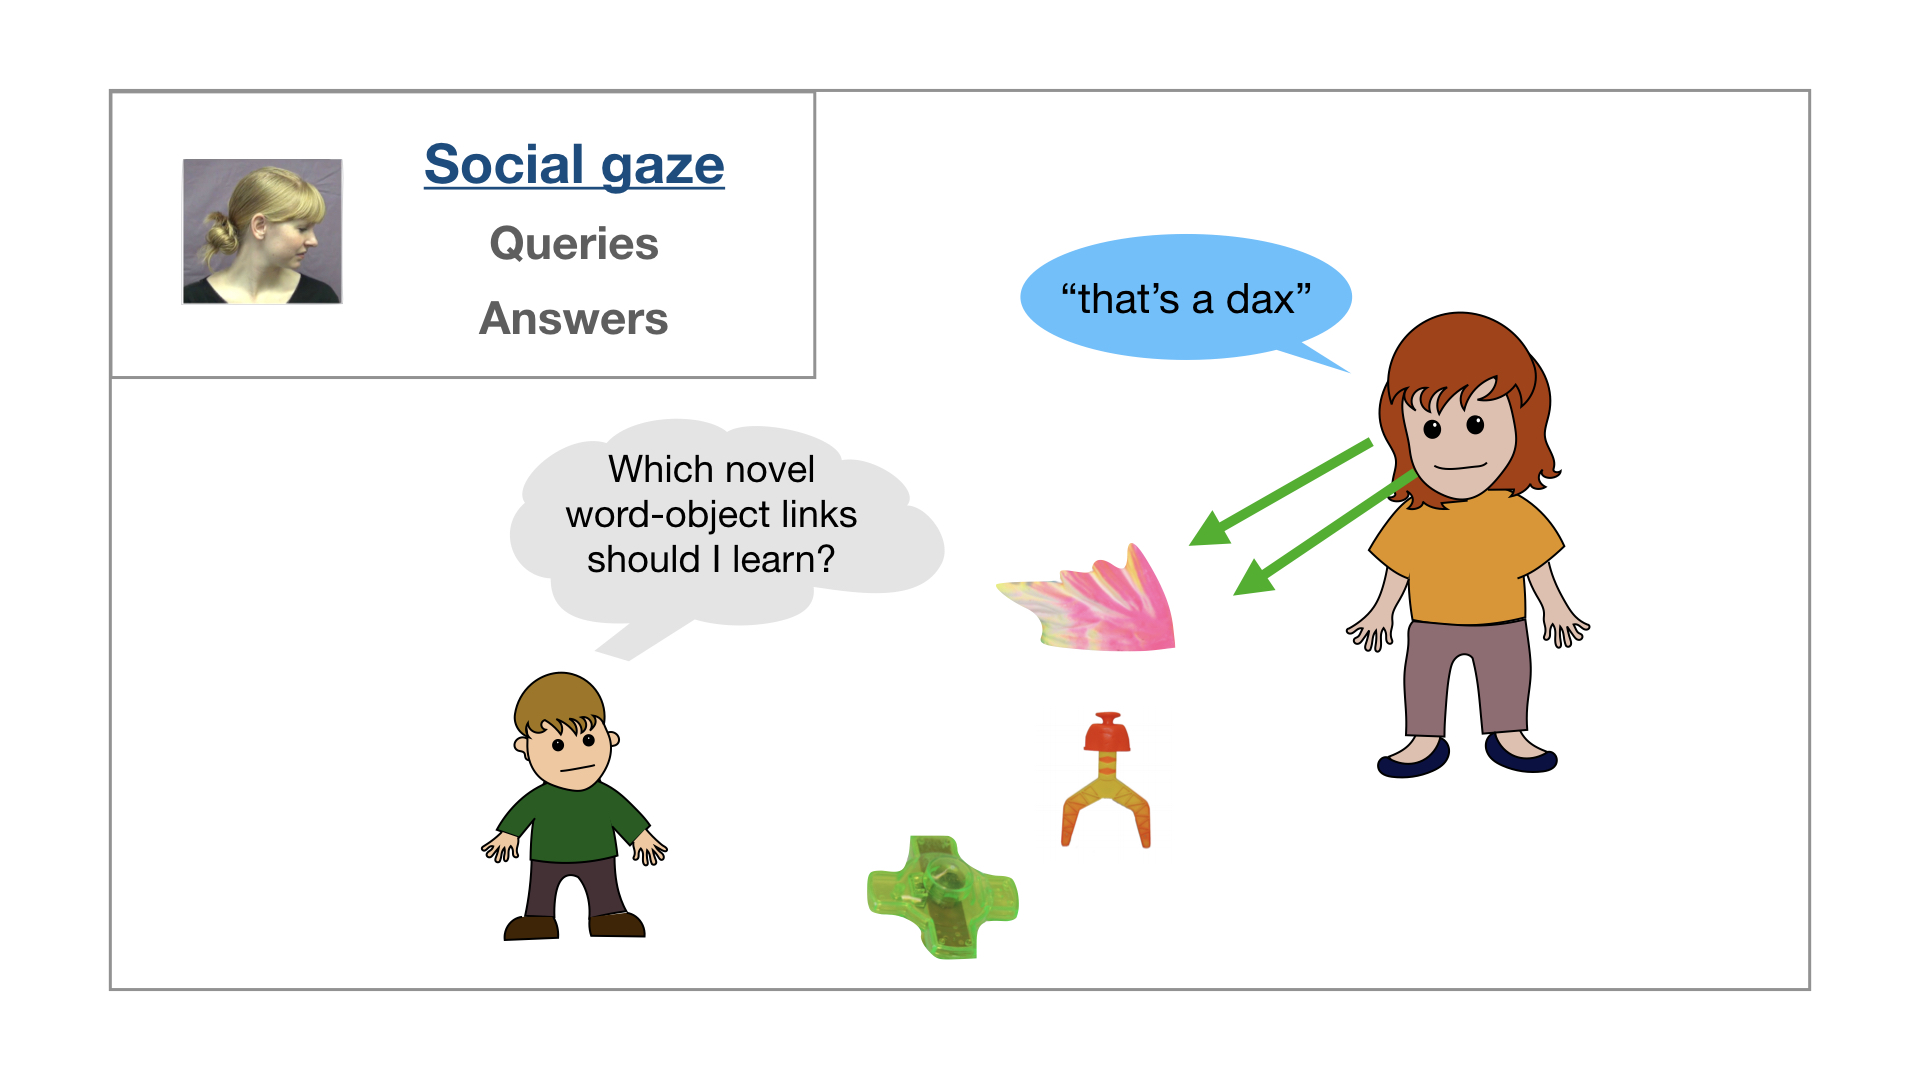
\includegraphics[width=0.95\linewidth]{/Users/ejyoon/Documents/Documents/Research/dissertation/index/chapter_child_rmds/SOC-XSIT/figures/soc_xsit} 

}

\caption[Overview of Chapter 4.]{A schematic showing the components of the active-social learning framework addressed by the case studies in Chapter 4.}\label{fig:schematic-soc-xsit}
\end{figure}
\section{Introduction}\label{introduction-2}

Learning the meaning of a new word should be hard. Consider that even
concrete nouns are often used in complex contexts with multiple possible
referents, which in turn have many conceptually natural properties that
a speaker could talk about. This ambiguity creates the potential for an
(in principle) unlimited amount of referential uncertainty in the
learning task.\footnote{This problem is a simplified version of Quine's
  \textit{indeterminacy of reference} (Quine, 1960): That there are many
  possible meanings for a word (``Gavigai'') that include the referent
  (``Rabbit'') in their extension, e.g., ``white,'' ``rabbit,''
  ``dinner.'' Quine's broader philosophical point was that different
  meanings (``rabbit'' and ``undetached rabbit parts'') could actually
  be extensionally identical and thus impossible to tease apart.}
Remarkably, word learning proceeds despite this uncertainty, with
estimates of adult vocabularies ranging between 50,000 to 100,000
distinct words (P. Bloom, 2002). How do learners infer and retain such a
large variety of word meanings from data with this kind of ambiguity?

Statistical learning theories offer a solution to this problem by
aggregating cross-situational statistics across labeling events to
identify underlying word meanings (Siskind, 1996; Yu \& Smith, 2007).
Recent experimental work has shown that both adults and young infants
can use word-object co-occurrence statistics to learn words from
individually ambiguous naming events (Smith \& Yu, 2008; Vouloumanos,
2008). For example, Smith and Yu (2008) taught 12-month-olds three novel
words simply by repeating consistent novel word-object pairings across
10 ambiguous exposure trials. Moreover, computational models suggest
that cross-situational learning can scale up to learn adult-sized
lexicons, even under conditions of considerable referential uncertainty
(K. Smith, Smith, \& Blythe, 2011).

Although all cross-situational learning models agree that the input is
the co-occurrence between words and objects and the output is stable
word-object mappings, they disagree about how closely learners
approximate the input distribution (for review, see Smith, Suanda, \& Yu
2014). One approach has been to model learning as a process of updating
connection strengths between multiple word-object links (McMurray,
Horst, \& Samuelson, 2012), while other approaches have argued that
learners store only a single word-object hypothesis (Trueswell, Medina,
Hafri, \& Gleitman, 2013). In recent experimental and modeling work
Yurovsky and Frank (2015) suggest an integrative explanation: learners
allocate a fixed amount of attention to a single hypothesis and
distribute the rest evenly among the remaining alternatives. As the set
of alternatives grows, the amount of attention allocated to each object
approaches zero.

In addition to the debate about representation, researchers have
disagreed about how to characterize the ambiguity of the input to
cross-situational learning mechanisms. One way to quantify the
uncertainty in a naming event is to show adults video clips of
caregiver-child interactions and measure their accuracy at guessing the
meaning of an intended referent (Human Simulation Paradigm: HSP
{[}Gillette, Gleitman, Gleitman, and Lederer, 1999{]}). Using the HSP,
Medina, Snedeker, Trueswell, and Gleitman (2011) found that
approximately 90\% of learning episodes were ambiguous (\textless{} 33\%
accuracy) and only 7\% were relatively unambiguous (\textgreater{} 50\%
accuracy). In contrast, Yurovsky, Smith, and Yu (2013) found a higher
proportion of clear naming events, with approximately 30\% being
unambiguous (\textgreater{} 90\% accuracy). Consistent with this
finding, Cartmill, Armstrong, Gleitman, Goldin-Meadow, Medina, and
Trueswell (2013) showed that the proportion of unambiguous naming
episodes varies across parent-child dyads, with some parents rarely
providing highly informative contexts and others' doing so relatively
more often.\footnote{The differences in the estimates of referential
  uncertainty in these studies could be driven by the different sampling
  procedures used to select naming events for the HSP. Yurovsky, Smith,
  and Yu (2013) sampled utterances for which the parent labeled a
  co-present object, whereas Medina, Snedeker, Trueswell, et al. (2011)
  randomly sampled any utterances containing concrete nouns. Regardless
  of these differences, the key point here is that variability in
  referential uncertainty across naming events exists and thus could
  alter the representations underlying cross-situational learning.}

Thus, representations in cross-situational word learning can appear
distributional or discrete, and the input to statistical learning
mechanisms can vary along a continuum from low to high ambiguity. These
results raise an interesting question: could learners be sensitive to
the ambiguity of the input and use this information to alter the
representations they store in memory? In the current line of work, we
investigated how the presence of referential cues in the social context
might alter the ambiguity of the input to statistical word learning
mechanisms.

Social-pragmatic theories of language acquisition emphasize the
importance of social cues for word learning (P. Bloom, 2002; E. V.
Clark, 2009; Hollich et al., 2000). Experimental work has shown that
even children as young as 16 months prefer to map novel words to objects
that are the target of a speaker's gaze and not their own (D. A.
Baldwin, 1993). In an analysis of naturalistic parent-child labeling
events, Yu and Smith (2012) found that young learners tended to retain
labels that were accompanied by clear referential cues, which served to
make a single object dominant in the visual field. And correlational
studies have demonstrated strong links between early intention-reading
skills (e.g., gaze following) and later vocabulary growth (Brooks \&
Meltzoff, 2005, 2008; Carpenter, Nagell, Tomasello, Butterworth, \&
Moore, 1998). Moreover, studies outside the domain of language
acquisition have shown that the presence of social cues: (a) produce
better spatial learning of audiovisual events (R. Wu, Gopnik,
Richardson, \& Kirkham, 2011), (b) boost recognition of a cued object
(Cleveland et al., 2007), and (c) lead to preferential encoding of an
object's featural information (J. M. Yoon et al., 2008). Together, the
evidence suggests that social cues could alter the representations
stored during cross-situational word learning by modulating how people
allocate attention to the relevant statistics in the input.

The goal of our current investigation was to ask whether the presence of
a valid social cue -- a speaker's gaze -- could change the
representations underlying cross-situational word learning. We used a
modified version of Yurovsky and Frank (2015)'s paradigm to provide a
direct measure of memory for alternative word-object links during
cross-situational learning. In Experiment 1, we manipulated the presence
of a referential cue at different levels of attention and memory
demands. At all levels of difficulty, learners tracked a strong single
hypothesis but were less likely to track multiple word-object links when
a social cue was present. In Experiment 2, we replicated the findings
from Experiment 1 using a more ecologically valid social cue. In
Experiment 3, we moved to a parametric manipulation of referential
uncertainty by varying the reliability of the speaker's gaze. Learners
were sensitive to graded changes in reliability and retained more
word-object links as uncertainty in the input increased. Finally, in
Experiment 4, we equated the length of the initial naming events with
and without the referential cue. Learners stored less information in the
presence of gaze even when they had visually inspected the objects for
the same amount of time. In sum, our data suggest that cross-situational
word learners are quite flexible, storing representations with different
levels of fidelity depending on the amount of ambiguity present during
learning.

\section{Experiment 1}\label{experiment-1}

We set out to test the effect of a referential cue on the
representations underlying cross-situational word learning. We used a
version of Yurovsky and Frank (2015)'s paradigm where we manipulated the
ambiguity of the learning context by including a gaze cue from a
schematic, female interlocutor. Participants saw a series of ambiguous
exposure trials where they heard one novel word that was either paired
with a gaze cue or not and selected the object they thought went with
each word. In subsequent test trials, participants heard the novel word
again, this time paired with a new set of novel objects. One of the
objects in this set was either the participant's initial guess (Same
test trials) or one of the objects was \emph{not} their initial guess
(Switch test trials). Performance on Switch trials provided a direct
measure of whether referential cues influenced the number of alternative
word-object links that learners stored in memory. If learners performed
worse on Switch trials after an exposure trial with gaze, this would
suggest that they stored fewer additional objects from the initial
learning context.

\subsection{Method}\label{method}

\subsubsection{Participants}\label{participants}

We posted a set of Human Intelligence Tasks (HITs) to Amazon Mechanical
Turk. Only participants with US IP addresses and a task approval rate
above 95\% were allowed to participate, and each HIT paid 30 cents.
50-100 HITs were posted for each of the 32 between-subjects conditions.
Data were excluded if participants completed the task more than once or
if participants did not respond correctly on familiar object trials (131
HITs). The final sample consisted of 1438 participants.
\begin{figure}[t]

{\centering 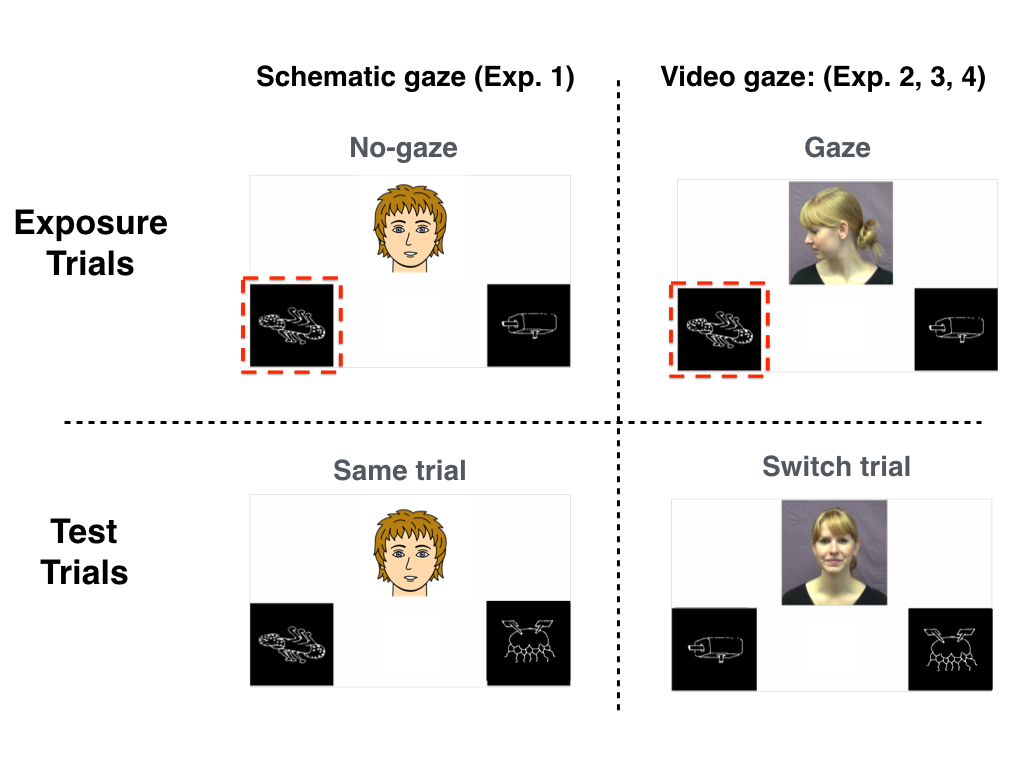
\includegraphics[width=0.95\linewidth]{/Users/ejyoon/Documents/Documents/Research/dissertation/index/chapter_child_rmds/SOC-XSIT/figures/stimuli_new} 

}

\caption[Examples of stimuli for exposure and test trials from Experiments 4.1-4.4.]{Screenshots of exposure and test trials from Experiments 1-4. The top left panel shows an exposure trial in the No-gaze condition using the schematic gaze cue (Experiment 4.1). The top right panel shows an exposure trial in the Gaze condition using the video gaze cue (Experiments 4.2-4.4). Participants saw either Gaze or No-gaze exposure trials depending on condition assignment, and participants saw both types of test trials: Same (bottom left panel) and Switch (bottom right panel). On Same trials, the object that participants chose during exposure appeared with a new novel object. On Switch trials the object that participants did not choose appeared with a new novel object. Participants either saw 2, 4, 6, or 8 referents on the screen depending on condition assignment.}\label{fig:stimuli}
\end{figure}
\subsubsection{Stimuli}\label{stimuli-1}

Figure 1 shows screenshots taken from Experiment 1. Visual stimuli were
black and white pictures of familiar and novel objects taken from
Kanwisher, Woods, Iacoboni, and Mazziotta (1997). Auditory stimuli were
recordings of familiar and novel words by an AT\&T Natural Voices
\texttrademark (voice: Crystal) speech synthesizer. Novel words were 1-3
syllable pseudowords that obeyed all rules of English phonotactics. A
schematic drawing of a human speaker was chosen for ease of manipulating
the direction of gaze, the referential cue of interest in this study.
All experiments can be viewed and downloaded at the project page:
\url{https://kemacdonald.github.io/soc_xsit/}.

\subsubsection{Design and Procedure}\label{design-and-procedure}

Participants saw a total of 16 trials: eight exposure trials and eight
test trials. On each trial, they heard one novel word, saw a set of
novel objects, and were asked to guess which object went with the word.
Before seeing exposure and test trials, participants completed four
practice trials with familiar words and objects. These trials
familiarized participants to the task and allowed us to exclude
participants who were unlikely to perform the task as directed, either
because of inattention or because their computer audio was turned off.

After the practice trials, participants were told that they would now
hear novel words and see novel objects and that their task was to select
the referent that ``goes with each word.'' Over the course of the
experiment, participants heard eight novel words two times, with one
exposure trial and one test trial for each word. Four of the test trials
were \emph{Same} trials in which the object that participants selected
on the exposure trial was shown with a set of new novel objects. The
other four test trials were \emph{Switch} trials in which one of the
objects was chosen at random from the set of objects that the
participant did not select on exposure.

Participants were randomly assigned to one of the 32 between-subjects
conditions (4 Referents X 4 Intervals X 2 Gaze conditions). Participants
either saw 2, 4, 6, or 8 referents on the screen and test trials
occurred at different intervals after exposure trials: either 0, 1, 3,
or 7 trials from the initial exposure to a word. For example, in the
0-interval condition, the test trial for that word would occur
immediately following the exposure trial, but in the 3-interval
condition, participants would see three additional exposure trials for
other novel words before seeing the test trial for the initial word. The
interval conditions modulated the time delay and the number of
intervening trials between learning and test, and the number of
referents conditions modulated the attention demands present during
learning.

Participants were assigned to either the Gaze or No-Gaze condition. In
the Gaze condition, gaze was directed towards one of the objects on
exposure trials; in the No-Gaze condition, gaze was always directed
straight ahead (see Figure 1 for examples). At test, gaze was always
directed straight ahead. To show participants that their response had
been recorded, a red box appeared around the selected object for one
second. This box always appeared around the selected object, even if
participants' selections were incorrect.

\subsection{Results and Discussion}\label{results-and-discussion}

\subsubsection{Analysis plan}\label{analysis-plan-1}

The structure of our analysis plan is parallel across all four
experiments. First, we examined accuracy on exposure trials in the Gaze
condition and then we compared response times on exposure trials across
the Gaze and No-Gaze conditions. These analyses tested whether learners
were (a) sensitive to our experimental manipulation and (b) altered
their allocation of attention in response to the presence of a social
cue. Accuracy on exposure trials was defined as selecting the referent
that was the target of gaze in the Gaze condition. (Note that there was
no ``correct'' behavior for exposure trials in the No-Gaze condition.)
Next, we examined accuracy on test trials to test whether learners'
memory for alternative word-object links changed depending on the
ambiguity of the learning context. Accuracy on test trials (both Same
and Switch) was defined as selecting the referent that was present
during the exposure trial for that word.

The key behavioral prediction of our hypothesis was that the presence of
gaze would result in reduced memory for multiple word-object links,
operationalized as a decrease in accuracy on Switch test trials after
seeing exposure trials with a gaze cue. To quantify participants'
behavior, we used mixed-effects regression models with the maximal
random effects structure justified by our experimental design:
by-subject intercepts and slopes for each trial type (Barr, Levy,
Scheepers, \& Tily, 2013). We limited all models to include only two-way
interactions because the critical test of our hypothesis was the
interaction between gaze condition and trial type, and we did not have
theoretical predictions for any possible three-way or four-way
interactions.

In the main text, we only report effects that achieved statistical
significance at the \(\alpha\) = .05 threshold. In the Appendix, we
report the full model specification and output for each of the models in
the paper. All models were fit using the lme4 package in R (Bates,
Maechler, Bolker, \& Walker, 2013), and all of our data and our
processing/analysis code can be viewed in the version control repository
for this paper at \url{https://github.com/kemacdonald/soc_xsit}.
\begin{figure}[t]

{\centering 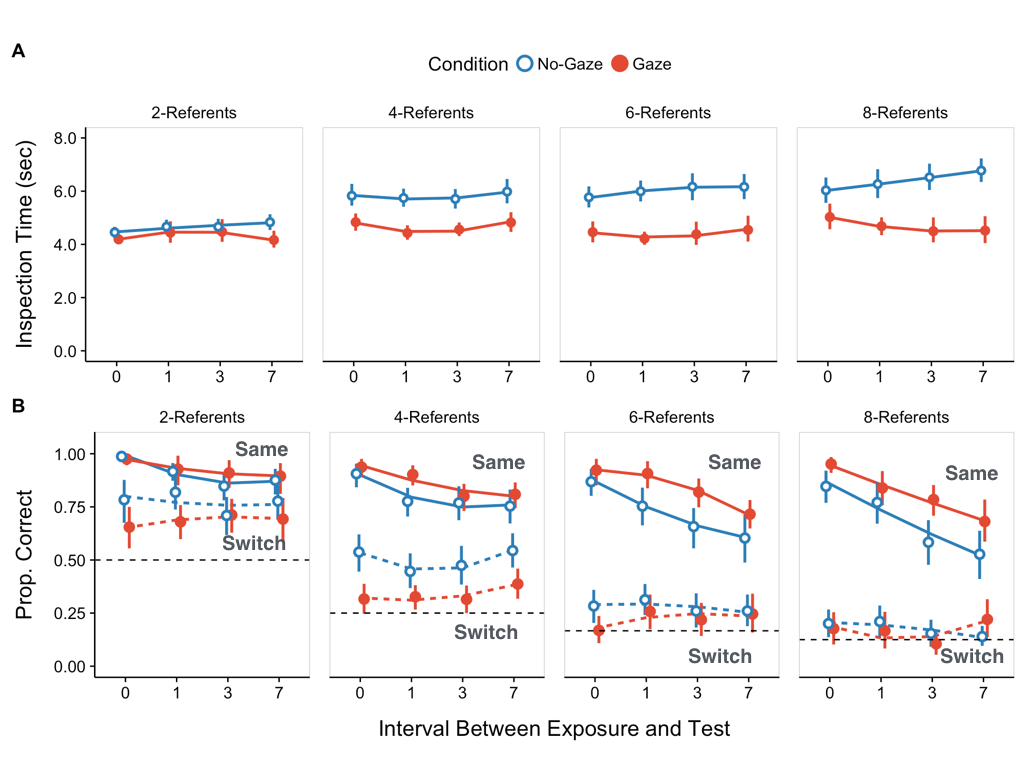
\includegraphics[width=0.95\linewidth]{/Users/ejyoon/Documents/Documents/Research/dissertation/index/chapter_child_rmds/SOC-XSIT/figures/expt1_new} 

}

\caption[Experiment 4.1 results.]{Experiment 4.1 results. The top row shows average inspection times on exposure trials for all experimental conditions as a function of the number of trials that occurred between exposure and test. Each panel represents a different number of referents, and line color represents the Gaze and No-Gaze conditions. The bottom row shows accuracy on test trials for all conditions as a function of the number of intervening trials. The horizontal dashed lines represent chance performance for each number of referents, and the type of line (solid vs. dashed) represents the different test trial types (Same vs. Switch). Error bars indicate 95\% confidence intervals computed by non-parametric bootstrap.}\label{fig:expt1-plot}
\end{figure}
\subsubsection{Exposure trials}\label{exposure-trials}

To ensure that our referential cue manipulation was effective, we
compared participants' accuracies on exposure trials in the Gaze
condition to a model of random behavior defined as a Binomial
distribution with a probability of success \(\frac{1}{Num Referents}\).
Correct performance was defined as selecting the object that was the
target of the speaker's gaze. Following Yurovsky and Frank (2015), we
fit logistic regressions for each gaze, referent, and interval
combination specified as
\texttt{Gaze Target $\sim$ 1 + offset(logit(1/Referents))}. The offset
encoded the chance probability of success given the number of referents,
and the coefficient for the intercept term shows on a log-odds scale how
much more likely participants were to select the gaze target than would
be expected if participants were selecting randomly. In all conditions,
participants used gaze to select referents on exposure trials more often
than expected by chance (smallest \(\beta\) = 1.4, z = 9.38, \(p\)
\textless{} .001). However, the mean proportion of gaze following varied
across conditions (overall \(M\) = 0.84, range: 0.77--0.93).

We were also interested in differences in participants' response times
across the experimental conditions. Since these trials were self-paced,
participants could choose how much time to spend inspecting the
referents on the screen, thus providing an index of participants'
attention. To quantify the effects of gaze, interval, and number of
referents, we fit a linear mixed-effects model that predicted
participants' inspection times as follows:
\texttt{Log(Inspection time) $\sim$ (Gaze * Log(Interval) + Log(Referents))$^2$ + (1 | subject)}.
We found a significant main effect of the number of referents (\(\beta\)
= 0.34, p \textless{} .001) with longer inspection times as the number
of referents increased, a significant interaction between gaze condition
and the number of referents (\(\beta\) = -0.27, p \textless{} .001) with
longer inspection times in the No-Gaze condition, especially as the
number of referents increased, and a significant interaction between
gaze condition and interval (\(\beta\) = -0.08, \(p\) = 0.004) with
longer inspection times in the No-Gaze condition, especially as the
number of intervening trials increased (see the top row of Figure 2).
Shorter inspection times on exposure trials with gaze provide evidence
that the presence of a referential cue focused participants' attention
on a single referent and away from alternative word-object links.

\subsubsection{Test trials}\label{test-trials}

Next, we explored participants' accuracy in identifying the referent for
each word in all conditions for both kinds of test trials (see the
bottom row of Figure 2). We first compared the distribution of correct
responses made by each participant to the distribution expected if
participants were selecting randomly defined as a Binomial distribution
with a probability of success \(\frac{1}{Num Referents}\). Correct
performance was defined as selecting the object that was present on the
exposure trial for that word. We fit the same logistic regressions as we
did for exposure trials:
\texttt{Correct $\sim$ 1 + offset(logit(1/Referents))}. In 31 out of the
32 conditions for both Same and Switch trials, participants chose the
correct object more often than would be expected by chance (smallest
\(\beta\) = 0.36, \(z\) = 2.44, \(p\) = 0.01). On Switch trials in the
8-referent, 3-interval condition, participants' responses were not
significantly different from chance (\(\beta\) = 0.06, z = 0.33, \(p\) =
0.74). Participants' success on Switch trials replicates the findings
from Yurovsky and Frank (2015) and provides direct evidence that
learners encoded more than a single hypothesis in ambiguous word
learning situations even under high attentional and memory demands and
in the presence of a referential cue.
\begin{table}[tb]
\centering
\begin{tabular}{lrrrrl}
 Predictor & Estimate & Std. Error & $z$ value & $p$ value &  \\ 
  \hline
Intercept & 3.01 & 0.29 & 10.35 & $<$ .001 & *** \\ 
  Switch Trial & -1.36 & 0.24 & -5.63 & $<$ .001 & *** \\ 
  Gaze Condition & 0.12 & 0.26 & 0.47 & 0.64 &  \\ 
  Log(Interval) & -0.45 & 0.11 & -4.08 & $<$ .001 & *** \\ 
  Log(Referents) & 0.23 & 0.11 & 2.02 & 0.04 & * \\ 
  Switch Trial*Gaze Condition & -1.09 & 0.12 & -9.07 & $<$ .001 & *** \\ 
  Switch Trial*Log(Interval) & 0.52 & 0.05 & 9.50 & $<$ .001 & *** \\ 
  Switch Trial*Log(Referent) & -0.59 & 0.09 & -6.49 & $<$ .001 & *** \\ 
  Gaze Condition*Log(Interval) & 0.06 & 0.06 & 1.00 & 0.32 &  \\ 
  Gaze Condition*Log(Referent) & 0.20 & 0.09 & 2.15 & 0.03 & * \\ 
  Log(Interval)*Log(Referent) & -0.04 & 0.04 & -1.02 & 0.31 &  \\ 
   \hline
\end{tabular}
\caption{Predictor estimates with standard errors and significance information for a logistic mixed-effects model predicting word learning in Experiment 4.1.} 
\label{tab:exp1_reg}
\end{table}
To quantify the effects of gaze, interval, and number of referents on
the probability of a correct response, we fit the following
mixed-effects logistic regression model to a filtered dataset where we
removed participants who did not reliably select the object that was the
target of gaze on exposure trials:\footnote{We did not predict that
  there would be a subset of participants who would not follow the gaze
  cue, thus this filtering criterion was developed posthoc. However, we
  think that the filter is theoretically motivated because we would only
  expect to see an effect of gaze if participants actually used the gaze
  cue. The filter removed 94 participants (6\% of the sample). The key
  inferences from the data do not depend on this filtering criterion.}
\texttt{Correct $\sim$ (Trial Type + Gaze + Log(Interval) + Log(Referents))$^2$ + offset(logit($^1/_{Referents}$)) + (TrialType | subject)}.
We coded interval and number of referents as continuous predictors and
transformed these variables to the log scale.\footnote{If we allowed for
  three-way interactions in the model, the key interaction between gaze
  condition and trial type remained significant (\(\beta\) = -1.3, \(p\)
  = 0.006).}

Table 1 shows the output of the logistic regression. We found
significant main effects of the number of referents (\(\beta = 0.23\),
\(p\) \textless{} .001) and interval (\(\beta = -0.45\), \(p\)
\textless{} .001), such that as each of these factors increased,
accuracy on test trials decreased. We also found a significant main
effect of trial type (\(\beta = -1.36\), \(p\) \textless{} .001), with
worse performance on Switch trials. There were significant interactions
between trial type and interval (\(\beta = 0.52\), \(p\) \textless{}
.001), trial type and referents (\(\beta = -0.59\), \(p\) \textless{}
.001), and gaze condition and referents (\(\beta = 0.2\), \(p\)
\textless{} .05). These interactions can be interpreted as meaning: (a)
the interval between exposure and test affected Same trials more than
Switch trials, (b) the number of referents affected Switch trials more
than Same trials, and (c) participants performed slightly better at the
higher number of referents in the Gaze condition. The interactions
between gaze condition and referents and between referents and interval
were not significant. Importantly, we found the predicted interaction
between trial type and gaze condition (\(\beta = -1.09\), \(p\)
\textless{} .001), with participants in the Gaze condition performing
worse on Switch trials. This interaction provides direct evidence that
the presence of a referential cue reduces participants' memory for
alternative word-object links.

We were also interested in how the length of inspection times on
exposure trials would affect participants' accuracy at test. So we fit
an additional model where participants' inspection times were included
as a predictor. We found a significant interaction between inspection
time and gaze condition (\(\beta = -0.17\), \(p\) = 0.01) such that
longer inspection times provided a larger boost to accuracy in the
No-Gaze condition. Importantly, the key test of our hypothesis, the
interaction between gaze condition and trial type, remained significant
in this alternative version of the model (\(\beta\) = -1.02, \(p\) = p
\textless{} .001).

Taken together, the inspection time and accuracy analyses provide
evidence that the presence of a referential cue modulated learners'
attention during learning, and in turn made them less likely to track
multiple word-object links. We saw some evidence for a boost to
performance on Same trials in the Gaze condition at the higher number of
referent and interval conditions, but reduced tracking of alternatives
did not always result in better memory for learners' candidate
hypothesis. This finding suggests that the limitations on Same trials
may be different than those regulating the distribution of attention on
Switch trials.

There was relatively large variation in performance across conditions in
the group-level accuracy scores and in participants' tendency to
\emph{use} the referential cue on exposure trials. Moreover, we found a
subset of participants who did not reliably use the gaze cue at all. It
is possible that the effect of gaze was reduced because the referential
cue that we used -- a static schematic drawing of a speaker -- was
relatively weak compared to the cues present in real-world learning
environments. Thus we do not yet know how learners' memory for
alternatives during cross-situational learning would change in the
presence of a stronger and more ecologically valid referential cue. We
designed Experiment 2 to address this question.

\section{Experiment 2}\label{experiment-2}

In Experiment 2, we set out to replicate the findings from Experiment 1
using a more ecologically valid stimulus set. We replaced the static,
schematic drawing with a video of an actress. While these stimuli were
still far from actual learning contexts, they included a real person who
provided both a gaze cue and a head turn towards the target object. To
reduce the across-conditions variability that we found in Experiment 1,
we introduced a within-subjects design where each participant saw both
Gaze and No-Gaze exposure trials in a blocked design. We selected a
subset of the conditions from Experiment 1 and tested only the
4-referent display with 0 and 3 intervening trials as between-subjects
manipulations. Our goals were to replicate the reduction in learners'
tracking of alternative word-object links in the presence of a
referential cue and to test whether increasing the ecological validity
of the cue would result in a boost to the strength of learners' recall
of their candidate hypothesis.

\subsection{Method}\label{method-1}

\subsubsection{Participants}\label{participants-1}

Participant recruitment and inclusion/exclusion criteria were identical
to those of Experiment 1. 100 HITs were posted for each condition (1
Referent X 2 Intervals X 2 Gaze conditions) for a total of 400 paid HITs
(33 HITs excluded).

\subsubsection{Stimuli}\label{stimuli-2}

Audio and picture stimuli were identical to Experiment 1. The
referential cue in the Gaze condition was a video (see Figure 1). On
each exposure trial, the actress looked out at the participant with a
neutral expression, smiled, and then turned to look at one of the four
images on the screen. She maintained her gaze for 3 seconds before
returning to the center. On test trials, she looked straight ahead for
the duration of the trial.

\subsubsection{Design and Procedure}\label{design-and-procedure-1}

Procedures were identical to those of Experiment 1. The major design
change was a within-subjects manipulation of the gaze cue where each
participant saw exposure trials with and without gaze. The experiment
consisted of 32 trials split into 2 blocks of 16 trials. Each block
consisted of 8 exposure trials and 8 test trials (4 Same trials and 4
Switch trials) and contained only Gaze or No-gaze exposure trials. The
order of block was counterbalanced across participants.

\subsection{Results and Discussion}\label{results-and-discussion-1}

We followed the same analysis plan as in Experiment 1. We first analyzed
inspection times and accuracy on exposure trials and then analyzed
accuracy on test trials.

\subsubsection{Exposure trials}\label{exposure-trials-1}

Similar to Experiment 1, participants' responses on exposure trials
differed from those expected by chance (smallest \(\beta\) = 3.39, z =
31.99, \(p\) \textless{} .001), suggesting that gaze was effective in
directing participants' attention. Participants in Experiment 2 were
more consistent in their use of gaze with the video stimuli compared to
the schematic stimuli used in Experiment 1 (\(M_{Exp1}\) = 0.8,
\(M_{Exp2}\) = 0.91), suggesting that using a real person increased
participants' willingness to follow the gaze cue.

We replicated the findings from Experiment 1. Inspection times were
shorter when gaze was present (\(\beta\) = -1.1, \(p\) \textless{} .001)
and in the 3-interval condition (\(\beta\) = -0.48, \(p\) \textless{}
.001). The interaction between gaze and interval was not significant,
meaning that gaze had the same effect on participants' inspection times
at both intervals (see Panel A of Figure 3).
\begin{figure}[t]

{\centering 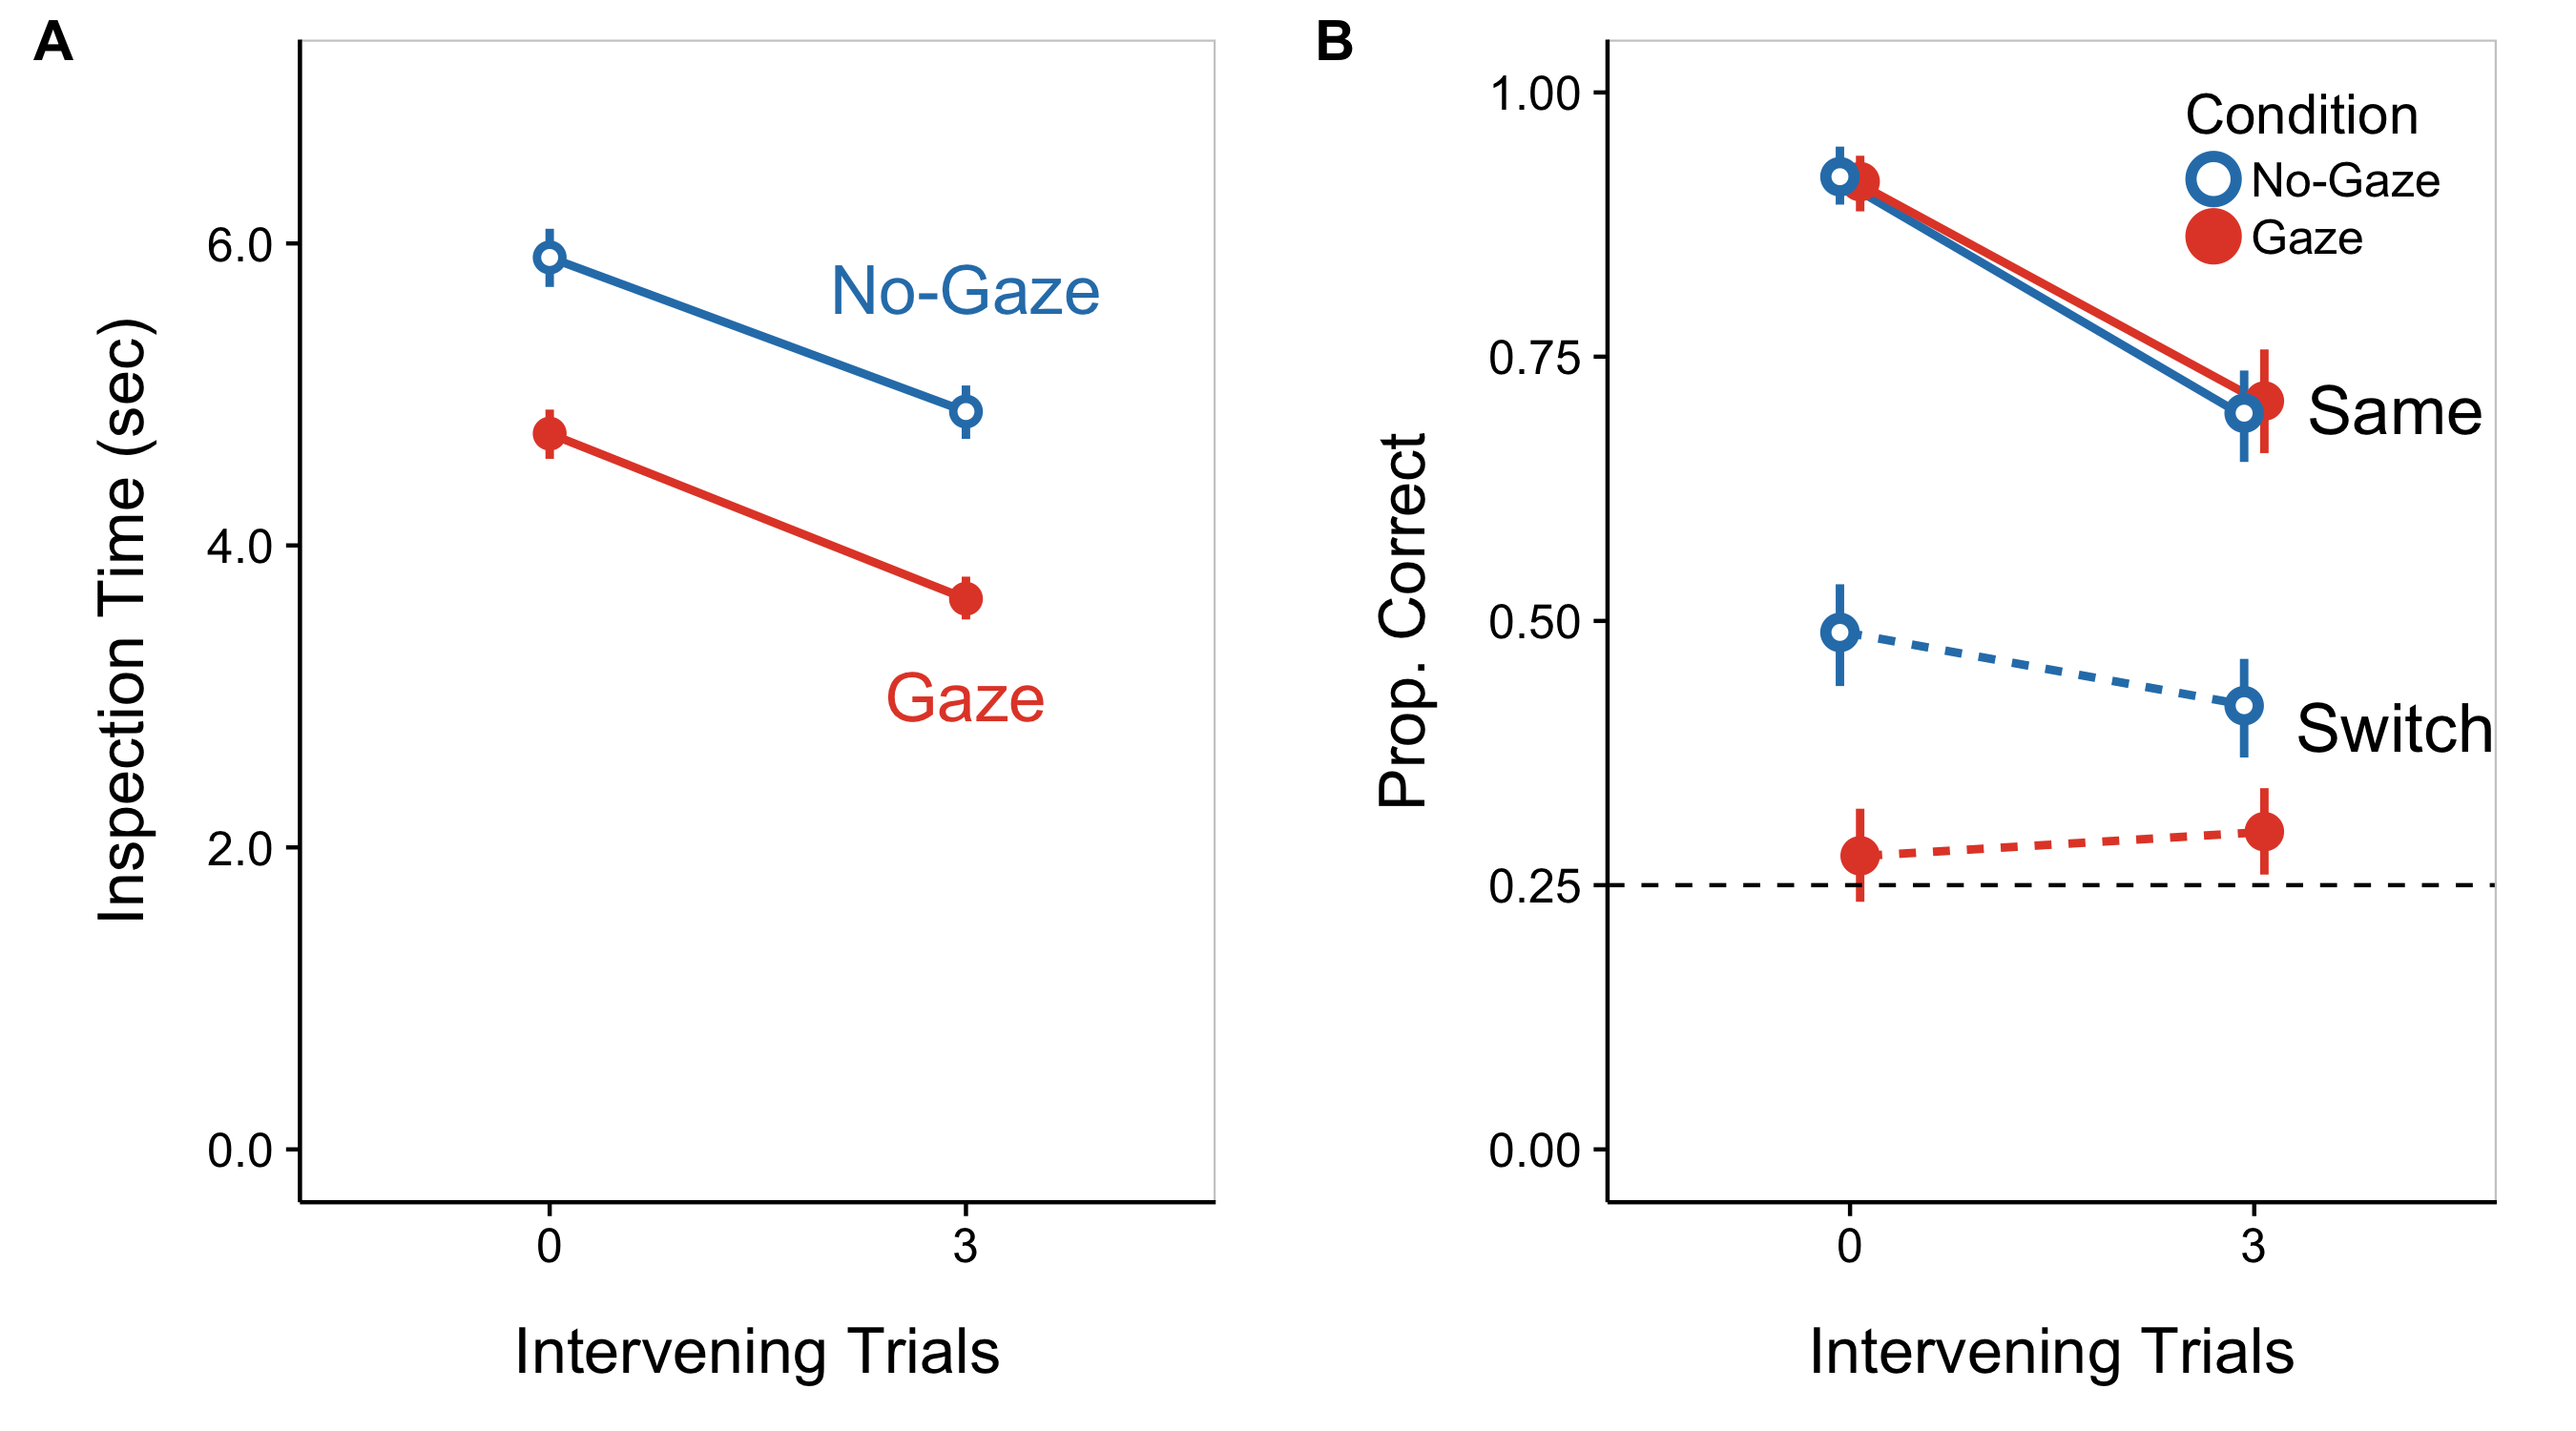
\includegraphics[width=0.95\linewidth]{/Users/ejyoon/Documents/Documents/Research/dissertation/index/chapter_child_rmds/SOC-XSIT/figures/expt2_new} 

}

\caption[Experiment 4.2 results]{Experiment 2 results. Panel A shows inspection times on exposure trials with and without gaze. Panel B shows accuracy on Same and Switch test trials. All plotting conventions are the same as in Figure 2. Error bars indicate 95\% confidence intervals computed by non-parametric bootstrap.}\label{fig:expt2-plot}
\end{figure}
\subsubsection{Test trials}\label{test-trials-1}
\begin{table}[tb]
\centering
\begin{tabular}{lrrrrl}
 Predictor & Estimate & Std. Error & $z$ value & $p$ value &  \\ 
  \hline
Intercept & 4.04 & 0.18 & 21.97 & $<$ .001 & *** \\ 
  Switch Trial & -2.99 & 0.19 & -16.11 & $<$ .001 & *** \\ 
  Gaze Condition & -0.10 & 0.16 & -0.63 & 0.53 &  \\ 
  Log(Interval) & -0.93 & 0.10 & -9.23 & $<$ .001 & *** \\ 
  Switch Trial*Gaze Condition & -0.71 & 0.16 & -4.49 & $<$ .001 & *** \\ 
  Switch Trial*Log(Interval) & 0.79 & 0.10 & 8.03 & $<$ .001 & *** \\ 
  Gaze Condition*Log(Interval) & 0.15 & 0.08 & 2.05 & 0.04 & * \\ 
   \hline
\end{tabular}
\caption{Predictor estimates with standard errors and significance information for a logistic mixed-effects model predicting word learning in Experiment 4.2.} 
\label{tab:exp2_reg}
\end{table}
Across all conditions for both trial types, participants selected the
correct referent at rates greater than chance (smallest \(\beta\) =
0.58, z = 9.32, \(p\) \textless{} .001). We replicated the critical
finding from Experiment 1: after seeing exposure trials with gaze,
participants performed worse on Switch trials, meaning they stored fewer
word-object links (\(\beta = -0.71\), \(p\) \textless{}
.001).\footnote{As in Experiment 1, we fit this model to a filtered dataset removing participants who did not reliably use the gaze cue.}
Participants were also less accurate as the interval between exposure
and test increased (\(\beta\) = -0.93, \(p\) \textless{} .001) and on
the Switch trials overall (\(\beta = -2.99\), \(p\) \textless{} .001).

In addition, there was a significant interaction between trial type and
interval (\(\beta = 0.79\), \(p\) \textless{} .001), with worse
performance on Switch trials in the 3-interval condition. The
interaction between gaze condition and interval was also significant
(\(\beta = 0.15\), \(p\) = 0.041), such that participants in the gaze
condition were less affected by the increase in interval. Similar to
Experiment 1, we did not see evidence of a boost to performance on Same
trials in the gaze condition.

Next, we added inspection times on exposure trials to the model. Similar
to Experiment 1, the key interaction between gaze and trial type
remained significant in this version of the model (\(\beta\) = -0.54,
\(p\) \textless{} .001). We also found an interaction between inspection
time and trial type (\(\beta\) = 0.21, \(p\) = 0.05), with longer
inspection times providing a larger boost to performance on Switch
trials (i.e., stronger memory for alternative word-object links). This
result differs slightly from Experiment 1 where we found an interaction
between trial type and inspection time, with longer inspection times
providing a larger boost to accuracy in the No-Gaze condition. Despite
this subtle difference, we speculate that inspection times likely played
a similar role in both experiments, with longer inspection times leading
to better performance on Switch trials since these trials depended on
encoding multiple word-object links. It is also possible that the
interaction between gaze condition and inspection time that we found in
Experiment 1 was influenced by the different number of referents and
interval conditions.

The results of Experiment 2 provide converging evidence for our primary
hypothesis that the presence of a referential cue reliably focuses
learners' attention away from alternative word-object links and shifts
them towards single hypothesis tracking. Moving to the video stimulus
led to higher rates of selecting the target of gaze on exposure trials,
but did not result in a boost to performance on Same trials. This
finding suggests that the level of attention and memory demand present
in the learning context might modulate the effect of gaze on the
fidelity of learners' single hypothesis.

Thus far we have shown that people store different amounts of
information in response to a categorical manipulation of referential
uncertainty. In both Experiments 1 and 2, the learning context was
either entirely ambiguous (No-Gaze) or entirely unambiguous (Gaze). But
not all real-world learning contexts fall at the extremes of this
continuum. Could learners be sensitive to more subtle changes in the
quality of the input? In our next experiment, we tested a prediction of
our account: whether learners would store more word-object links in
response to graded changes in referential uncertainty during learning.

\section{Experiment 3}\label{experiment-3}

In Experiment 3, we explored whether learners would allocate attention
and memory flexibly in response to \emph{graded} changes in the
referential uncertainty that was present during learning. To test this
hypothesis, we moved beyond a categorical manipulation of the
presence/absence of gaze, and we parametrically varied the reliability
of the referential cue. We manipulated cue reliability by adding a block
of familiarization trials where we varied the proportion of Same and
Switch trials. If participants saw more Switch trials, this provided
direct evidence that the speaker's gaze was a less reliable cue to
reference because the gaze target on exposure trials would not appear at
test. This design was inspired by a growing body of experimental work
showing that even young children are sensitive to the prior reliability
of speakers and will use this information to decide whom to learn novel
words from (e.g., Koenig, Clement, \& Harris, 2004).

\subsection{Method}\label{method-2}

\subsubsection{Participants}\label{participants-2}

Participant recruitment and inclusion/exclusion criteria were identical
to those of Experiment 1 and 2 (27 HITs excluded). 100 HITs were posted
for each reliability level (0\%, 25\%, 50\%, 75\%, and 100\%) for total
of 500 paid HITs.

\subsubsection{Design and Procedure}\label{design-and-procedure-2}

Procedures were identical to those of Experiments 1 and 2. We modified
the design of our cross-situational learning paradigm to include a block
of 16 familiarization trials (8 exposure trials and 8 test trials) at
the beginning of the experiment. These trials served to establish the
reliability of the speaker's gaze. To establish reliability, we varied
the proportion of Same/Switch trials that occurred during the
familiarization block. Recall that on Switch trials the gaze target did
not show up at test, which provided evidence that the speaker's gaze was
not a reliable cue to reference. Reliability was a between-subjects
manipulation such that participants either saw 8, 6, 4, 2, or 0 Switch
trials during familiarization, which created the 0\%, 25\%, 50\%, 75\%,
and 100\% reliability conditions. After the familiarization block,
participants completed another block of 16 trials (8 exposure trials and
8 test trials). Since we were no longer testing the effect of the
presence or absence of a referential cue, all exposure trials throughout
the experiment included a gaze cue. Finally, at the end of the task, we
asked participants to assess the reliability of the speaker on a
continuous scale from ``completely unreliable'' to ``completely
reliable.''

\subsection{Results and Discussion}\label{results-and-discussion-2}

\subsubsection{Exposure trials}\label{exposure-trials-2}

Participants reliably chose the referent that was the target of gaze at
rates greater than chance (smallest \(\beta\) = 2.62, z = 31.99, \(p\)
\textless{} .001). We fit a mixed effects logistic regression model
predicting the probability of selecting the gaze target as follows:
\texttt{Correct-Exposure $\sim$ Reliability Condition * Subjective Reliability + (1 | subject)}.
We found an effect of reliability condition (\(\beta\) = 3.28, \(p\) =
0.03) such that when the gaze cue was more reliable, participants were
more likely to use it (\(M_{0\%}\) = 0.83, \(M_{25\%}\) = 0.82,
\(M_{50\%}\) = 0.87, \(M_{75\%}\) = 0.9, \(M_{100\%}\) = 0.94). We also
found an effect of subjective reliability (\(\beta\) = 7.26, \(p\)
\textless{} .001) such that when participants thought the gaze cue was
reliable, they were more likely to use it. This analysis provides
evidence that participants were sensitive to the reliability
manipulation both in how often they used the gaze cue and in how they
rated the reliability of the speaker at the end of the task.

\subsubsection{Test trials}\label{test-trials-2}
\begin{figure}[t]

{\centering 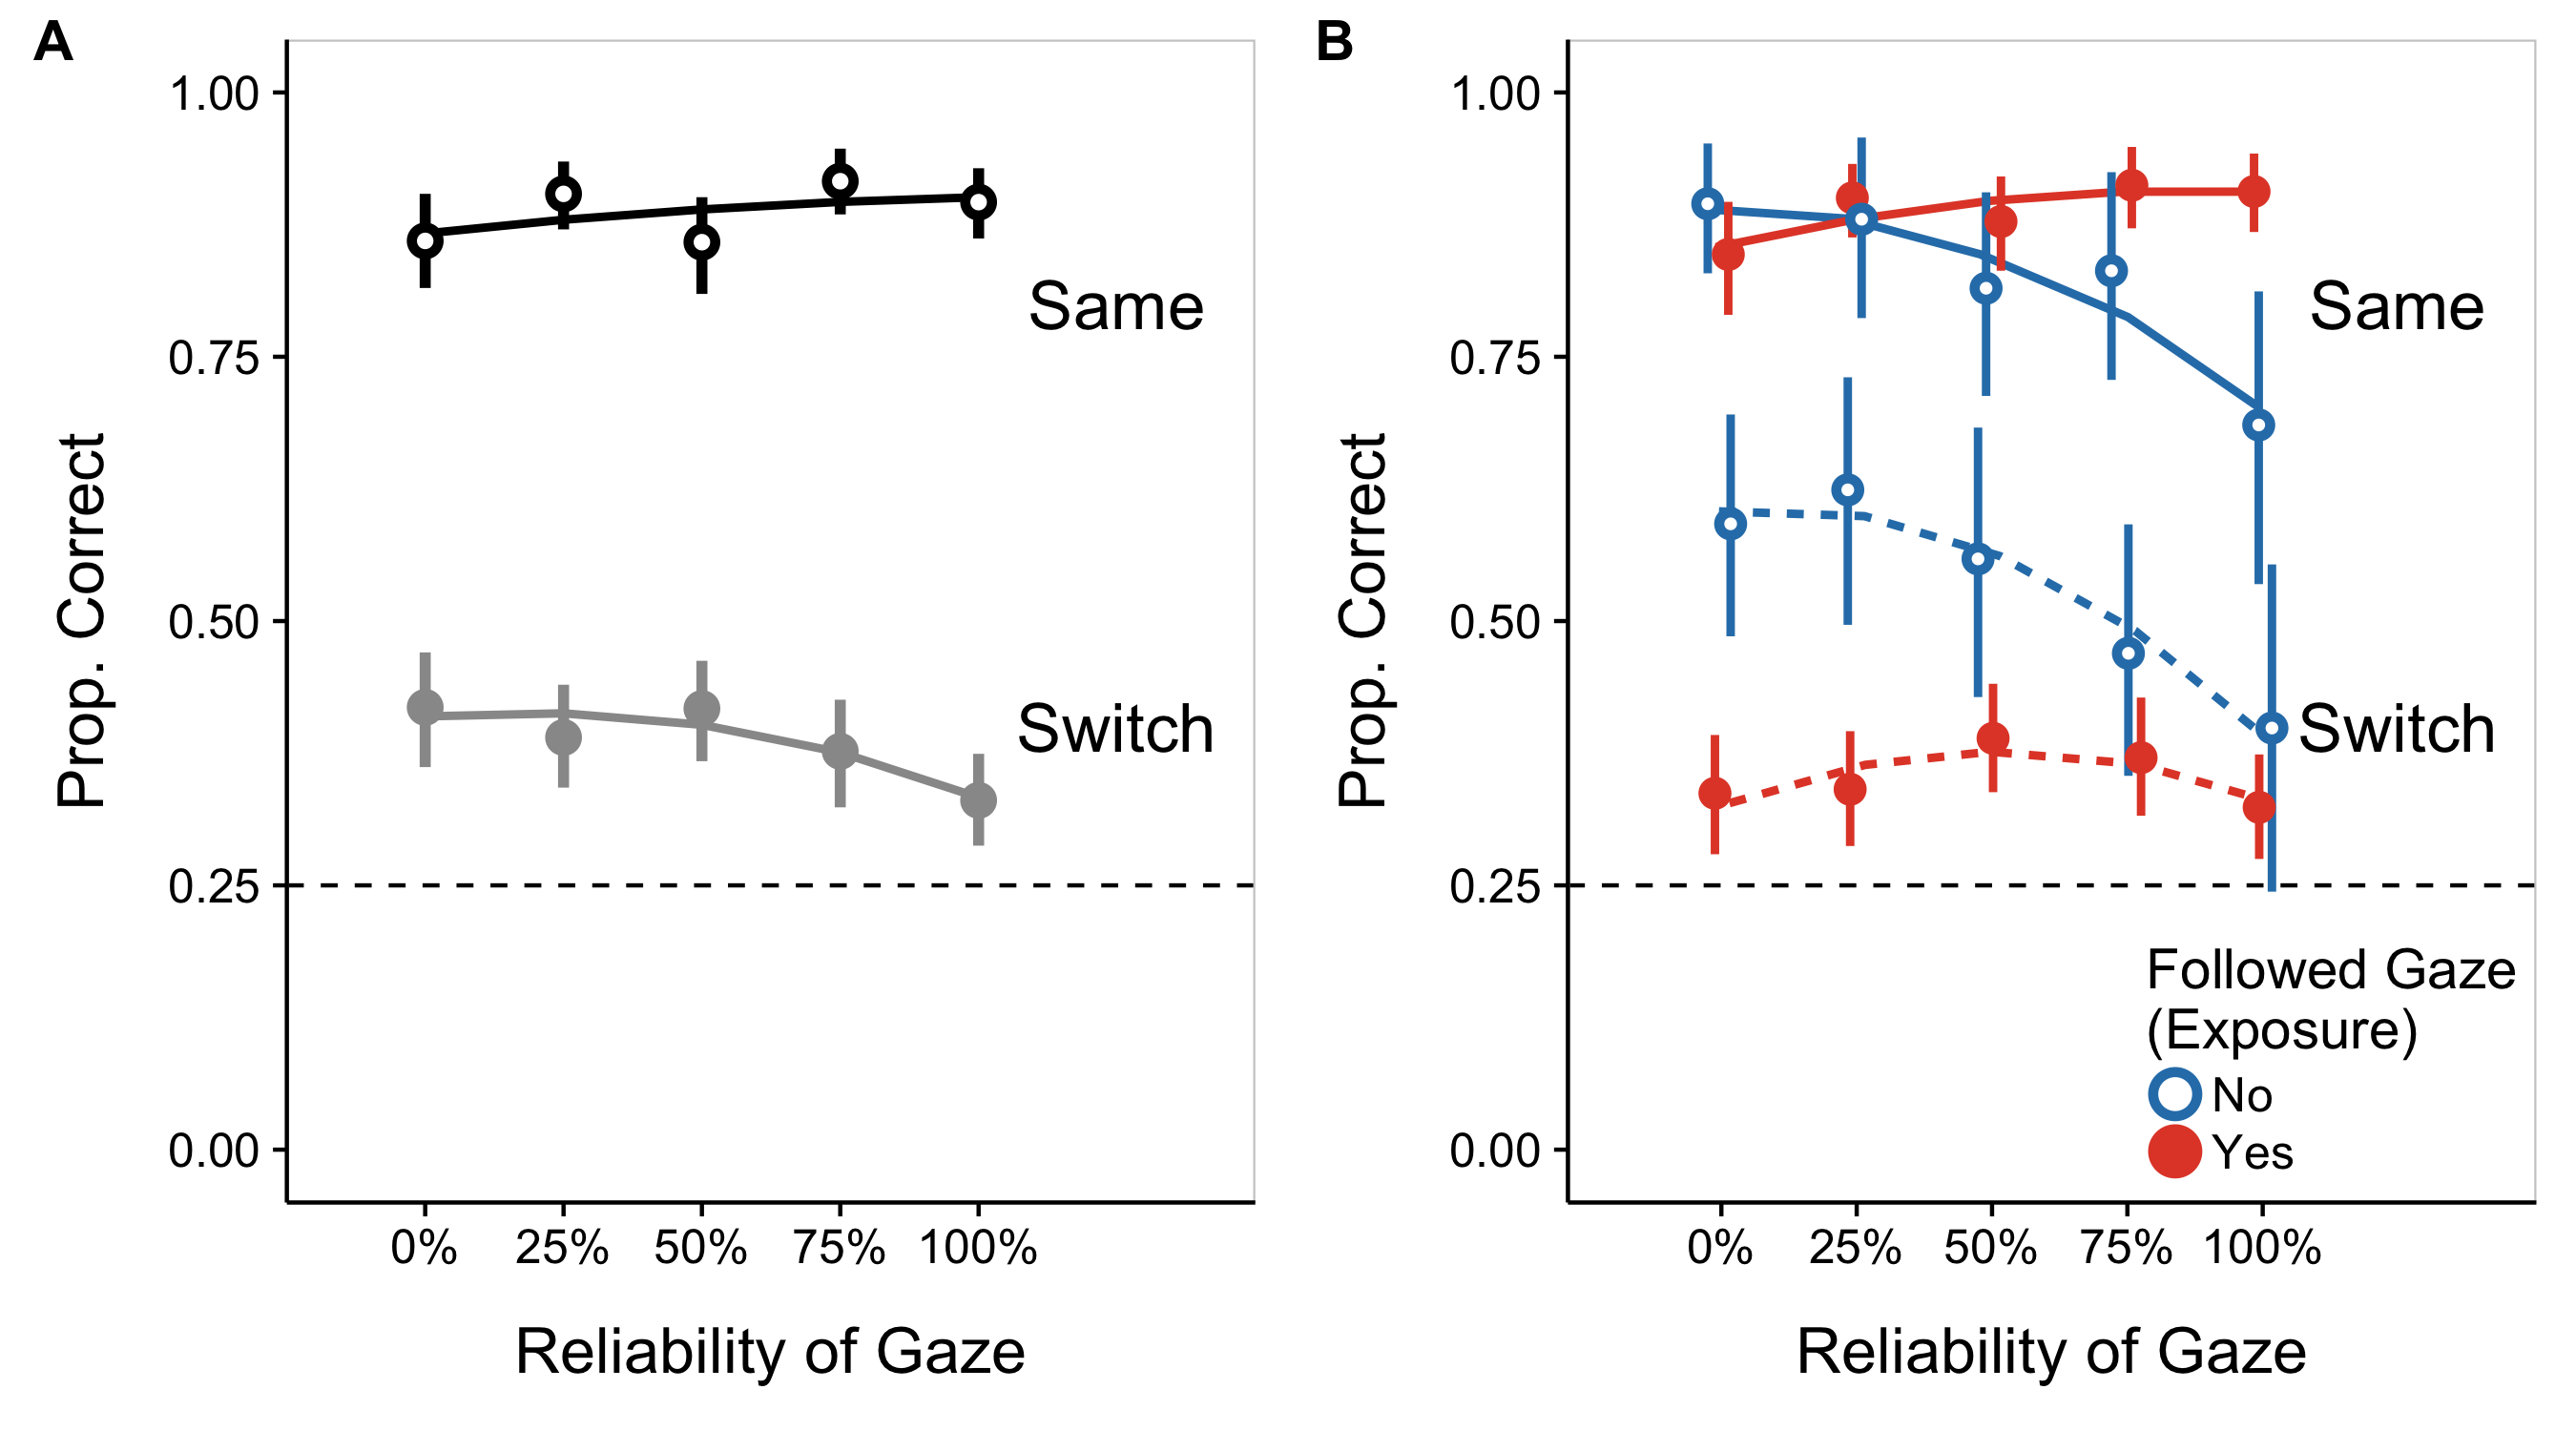
\includegraphics[width=0.95\linewidth]{/Users/ejyoon/Documents/Documents/Research/dissertation/index/chapter_child_rmds/SOC-XSIT/figures/expt3_main_plot} 

}

\caption[Primary analyses of test trial performance in Experiment 4.3]{Primary analyses of test trial performance in Experiment 3. Panel A shows performance as a function of reliability condition. Panel B shows performance as a function of reliability condition and whether participants chose to follow gaze on exposure trials. The horizontal dashed lines represent chance performance, and error bars indicate 95\% confidence intervals computed by non-parametric bootstrap.}\label{fig:e3-plot}
\end{figure}
Next, we tested whether the reliability manipulation altered the
strength of participants' memory for alternative word-object links in
the second block of test trials that followed the initial
familiarization phase. Across all conditions, participants selected the
correct referent at rates greater than chance (smallest \(\beta\) =
0.42, z = 3.69, \(p\) \textless{} .001). Our primary prediction was an
interaction between reliability and test trial type, with higher levels
of reliability leading to worse performance on Switch trials (i.e., less
memory allocated to alternative word-object links). To explore this
prediction, we performed four complementary analyses: our primary
analysis, which tested the effect of the reliability manipulation, and
three secondary analyses, which explored the effects of participants'
(a) use of the gaze cue, (b) subjective reliability assessments, and (c)
inspection time on exposure trials.
\begin{figure}[t]

{\centering 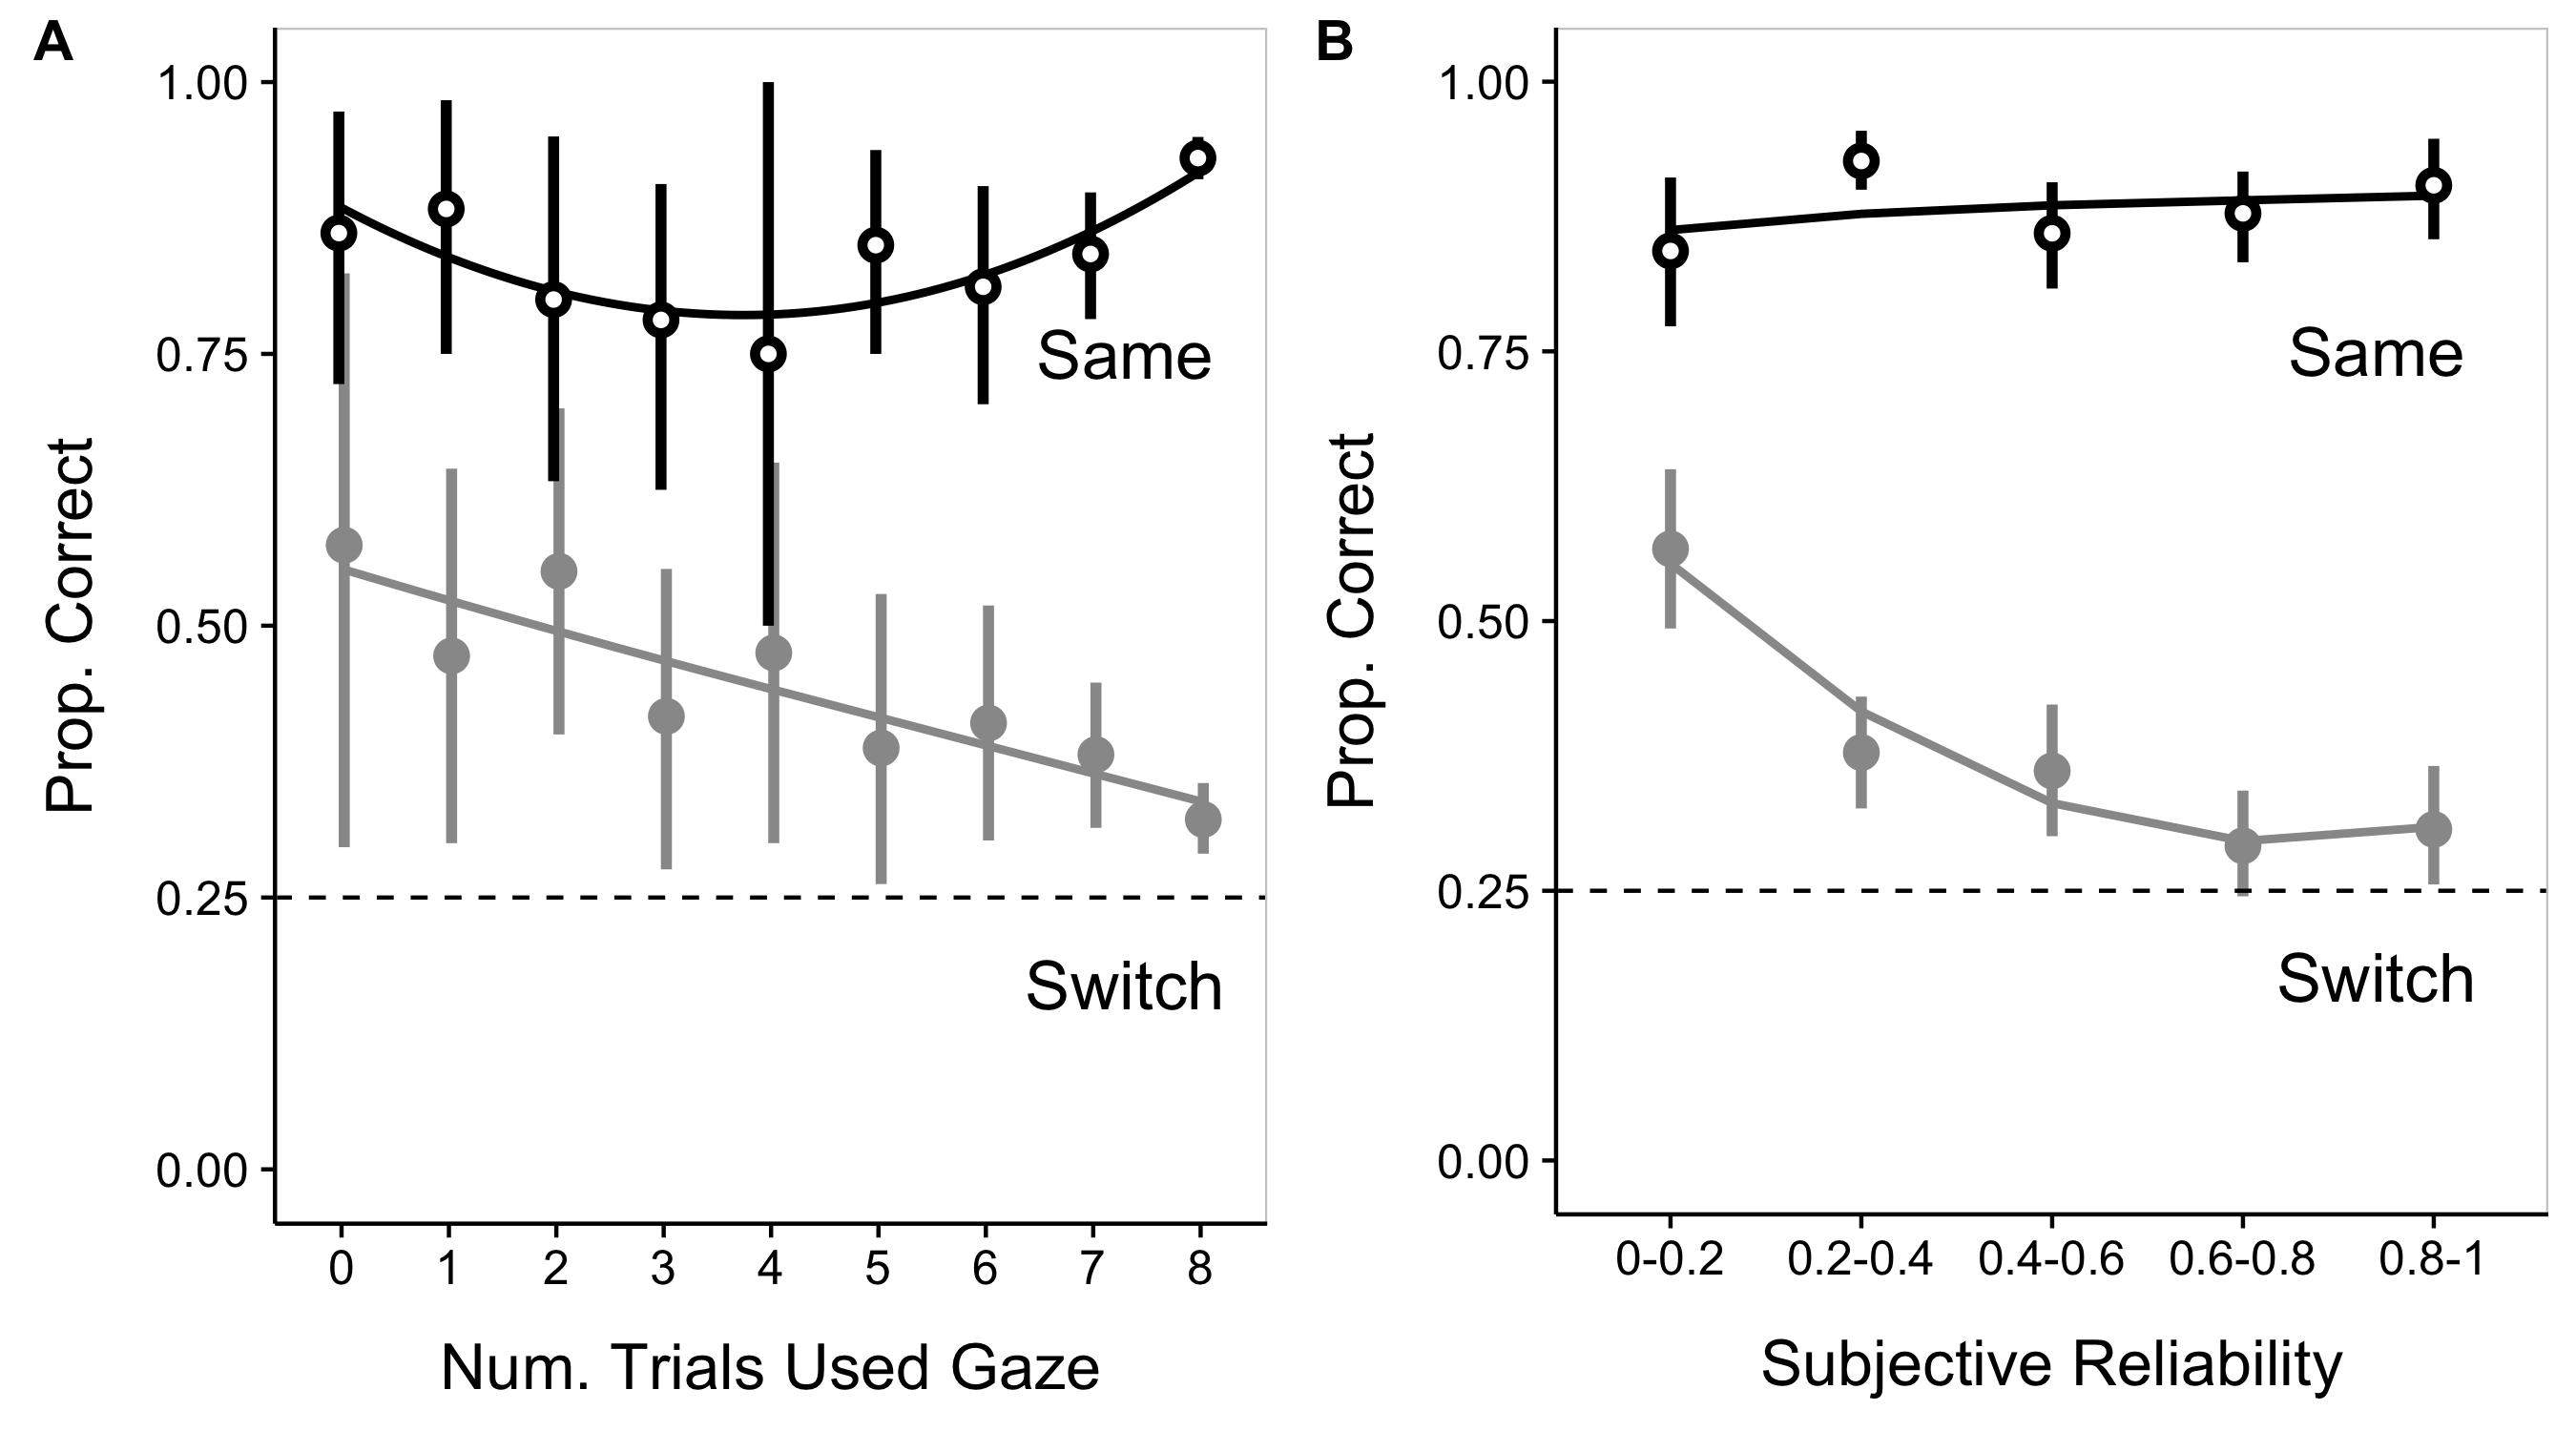
\includegraphics[width=0.95\linewidth]{/Users/ejyoon/Documents/Documents/Research/dissertation/index/chapter_child_rmds/SOC-XSIT/figures/expt3_sub_plot} 

}

\caption[Secondary analyses of test trial performance in Experiment 4.3]{Secondary analyses of test trial performance in Experiment 3. Panel A shows accuracy as a function of the number of exposure trials on which participants chose to use the gaze cue. Panel B shows accuracy as a function of participants' subjective reliability judgments. The horizontal dashed lines represent chance performance, and error bars indicate 95\% confidence intervals computed by non-parametric bootstrap.}\label{fig:expt3-sub-plots}
\end{figure}
\subsubsection{Reliability condition
analysis}\label{reliability-condition-analysis}

To test the effect of reliability, we fit a model predicting accuracy at
test using reliability condition and test trial type as predictors. We
found a significant main effect of trial type (\(\beta = -3.95\), \(p\)
\textless{} .001), with lower accuracy on Switch trials. We also found
the key interaction between reliability condition and trial type
(\(\beta\) = -0.76, \(p\) = 0.044), such that when gaze was more
reliable, participants performed worse on Switch trials (see Panel A of
Figure 4). This interaction suggests that people store more word-object
links as the learning context becomes more ambiguous. However, the
interaction between reliability and trial type was not particularly
strong, and -- similar to Experiment 1 -- performance varied across
conditions (see the 50\% reliable condition in Panel A of Figure 4). So
to provide additional support for our hypothesis, we conducted three
follow-up analyses.

\subsubsection{Gaze use analyses}\label{gaze-use-analyses}

We would only expect to see a strong interaction between reliability and
trial type if learners chose to use the gaze cue during exposure trials.
To test this hypothesis, we fit two additional models that included two
different measures of participants' use of the gaze cue. First, we added
the number of exposure trials on which participants chose to use the
gaze cue as a predictor in our model. We found a significant interaction
between use of the gaze cue on exposure trials and trial type
(\(\beta = -1.43\), \(p\) \textless{} .001) with worse performance on
Switch test trials when participants used gaze on exposure trials (see
Panel B of Figure 4). We also found an interaction between gaze use and
reliability (\(\beta = 0.97\), \(p\) = 0.004) such that when gaze was
more reliable, participants were more likely to use it. The \(\beta\)
value for the interaction between trial type and reliability changed
from -0.76 to -0.62, (\(p\) = 0.086). This reduction suggests that
participants' tendency to use the gaze cue is a stronger predictor of
learners' memory for alternative word-object links compared to our
reliability manipulation.\footnote{We are grateful to an anonymous
  reviewer for suggesting this analysis, but we would like to note that
  it is exploratory.}

We also hypothesized that the reliability manipulation might change how
often individual participants chose to use the gaze cue throughout the
task. To explore this possibility, we fit a model with the same
specifications, but we included a predictor that we created by binning
participants based on the number of exposure trials on which they chose
to follow gaze (i.e., a gaze following score). We found a significant
interaction between how often participants chose to follow gaze on
exposure trials and trial type (\(\beta = -0.26\), \(p\) \textless{}
.001), such that participants who were more likely to use the gaze cue
performed worse on Switch trials, but not Same trials (see Panel A of
Figure 5).\footnote{We found this interaction while performing
  exploratory data analyses on a previous version of this study with an
  independent sample (N = 250, \(\beta = -0.24\), \(p\) \textless{}
  .001). The results reported here are from a follow-up study where
  testing this interaction was a planned analysis.} Taken together, the
two analyses of participants' use of the gaze cue provide converging
evidence that when the speaker's gaze was reliable participants were
more likely to use the cue, and when they followed gaze, they tended to
store less information from the initial naming event.

\subsubsection{Subjective reliability
analysis}\label{subjective-reliability-analysis}

The strong interaction between use of the gaze cue and memory for
alternative word-object links suggests that participants' subjective
experience of reliability in the experiment mattered. Thus, we fit the
same model but substituted subjective reliability for the frequency of
gaze use as a predictor of test trial performance. We found a
significant interaction between trial type and participants' subjective
reliability assessments (\(\beta = -1.63\), \(p\) = 0.01): when
participants thought the speaker was more reliable, they performed worse
on Switch trials, but not Same trials (see Panel B of Figure 5).

\subsubsection{Inspection time analyses}\label{inspection-time-analyses}

Finally, we analyzed the effect of inspection times on exposure trials,
fitting a model using inspection time, trial type, and reliability
condition to predict accuracy at test. We found a main effect of
inspection time (\(\beta\) = 0.31, \(p\) = 0.001), with longer
inspection times leading to better performance for both Same and Switch
trials. The interaction between inspection time and reliability
condition was not significant. The key interaction between reliability
condition and trial type remained significant in this version of the
model (\(\beta\) = -0.58, \(p\) = 0.048).

Next, we explored the factors that influenced inspection time on
exposure trials by fitting a model to predict inspection times as a
function of reliability condition and participants' use of the gaze cue.
We found a main effect of participants' use of the gaze cue (-0.32,
\(p\) \textless{} .001) with shorter inspection times when participants
followed gaze. The main effect of reliability condition and the
interaction between reliability and use of gaze were not significant.
These analyses provide evidence that inspection times were similar
across the different reliability conditions and that use of the gaze cue
was the primary factor affecting how long participants explored the
objects during learning.

Together, these four analyses show that when the speaker's gaze was more
reliable, participants were more likely to: (a) use the gaze cue, (b)
rate the speaker as more reliable, and (c) store fewer word-object
links, showing behavior more consistent with single hypothesis tracking.
These findings support and extend the results of Experiments 1 and 2 in
several important ways. First, similar to Experiment 2, participants'
performance on Same trials was relatively unaffected by changes in
performance on Switch trials. The selective effect of gaze on Switch
trials provides converging evidence that the limitations on Same trials
may be different than those regulating the distribution of attention on
Switch trials. Second, learners' use of a referential cue was a stronger
predictor of reduced memory for alternative word-object links compared
to our reliability manipulation. Although we found a significant effect
of reliability on participants' use of the gaze cue, participants'
tendency to use the cue remained high. Consider that even in the 0\%
reliability condition the mean proportion of gaze following was still
0.82. It is reasonable that participants would continue to use the gaze
cue in our experiment since it was the only cue available and
participants did not have a strong reason to think that the speaker
would be deceptive.

The critical contribution of Experiment 3 is to show that learners
respond to a graded manipulation of referential uncertainty, with the
amount of information stored from the initial exposure tracking with the
reliability of the cue. This graded accuracy performance shows that
learners stored alternative word-object links with different levels of
fidelity depending on the amount of referential uncertainty present
during learning.

Across Experiments 1-3, learners tended to store fewer word-object links
in unambiguous learning contexts when a clear referential cue was
present. However, in all three experiments, participants' responses on
exposure trials controlled the length of the trial, meaning that when
participants used the gaze cue, they also spent less time visually
inspecting the objects. Thus, we do not know whether there is an
independent effect of referential cues on the representations underlying
cross-situational learning, or if the effects found in Experiments 1-3
are entirely mediated by a reduction in inspection time. In Experiment
4, we addressed this possibility by removing participants' control over
the length of exposure trials, which made the inspection times
equivalent across the Gaze and No-Gaze conditions.

\section{Experiment 4}\label{experiment-4}

In Experiment 4, we asked whether a reduction in visual inspection time
in the gaze condition could completely explain the effect of social cues
on learners' reduced memory for alternative word-object links. To answer
this question, we modified our paradigm and made the length of exposure
trials equivalent across the Gaze and No-Gaze conditions. In this
version of the task, participants were shown the objects for a fixed
amount of time regardless of whether gaze was present. We also included
two different exposure trial lengths in order to test whether gaze would
have a differential effect at shorter vs.~longer inspection times. If
the presence of gaze reduces learners' memory for multiple word-object
links, then this provides evidence that referential cues affected the
underlying representations over and above a reduction in inspection
time.

\subsection{Method}\label{method-3}

\subsubsection{Participants}\label{participants-3}

Participant recruitment and inclusion/exclusion criteria were identical
to those of Experiments 1, 2, and 3. 100 HITs were posted for each
condition (1 Referent X 2 Intervals X 2 Inspection Time conditions) for
a total of 400 paid HITs (37 HITs excluded).

\subsubsection{Stimuli}\label{stimuli-3}

Audio, picture, and video stimuli were identical to Experiments 2 and 3.
Since inspection times were fixed across conditions, we wanted to ensure
that participants were aware of the time remaining on each exposure
trial. So we included a circular countdown timer located above the
center video. The timer remained on the screen during test trials but
did not count down since participants could take as much time as they
wanted to respond on test trials.

\subsubsection{Design and Procedure}\label{design-and-procedure-3}

Procedures were identical to those of Experiment 1-3. The design was
identical to that of Experiment 2 and consisted of 32 trials split into
2 blocks of 16 trials. Each block consisted of 8 exposure trials and 8
test trials (4 Same trials and 4 Switch trials) and contained only Gaze
or No-Gaze exposure trials. The order of block was counterbalanced
across participants.

The major design change was to make the length of exposure trials
equivalent across the Gaze and No-Gaze conditions. We randomly assigned
participants to one of two inspection time conditions: Short or Long.
Initially, the length of the inspection times was based on participants'
self-paced inspection times in the Gaze and No-Gaze conditions in
Experiment 2 (Short = 3 seconds; Long = 6 seconds). However, after pilot
testing, we added three seconds to each condition to ensure that
participants had enough time to respond before the experiment advanced
(Short = 6 seconds; Long = 9 seconds). If participants did not respond
in the allotted time, an error message appeared informing participants
that time had run out and encouraged them to respond within the time
window on subsequent trials.

\subsection{Results and Discussion}\label{results-and-discussion-3}
\begin{figure}[t]

{\centering 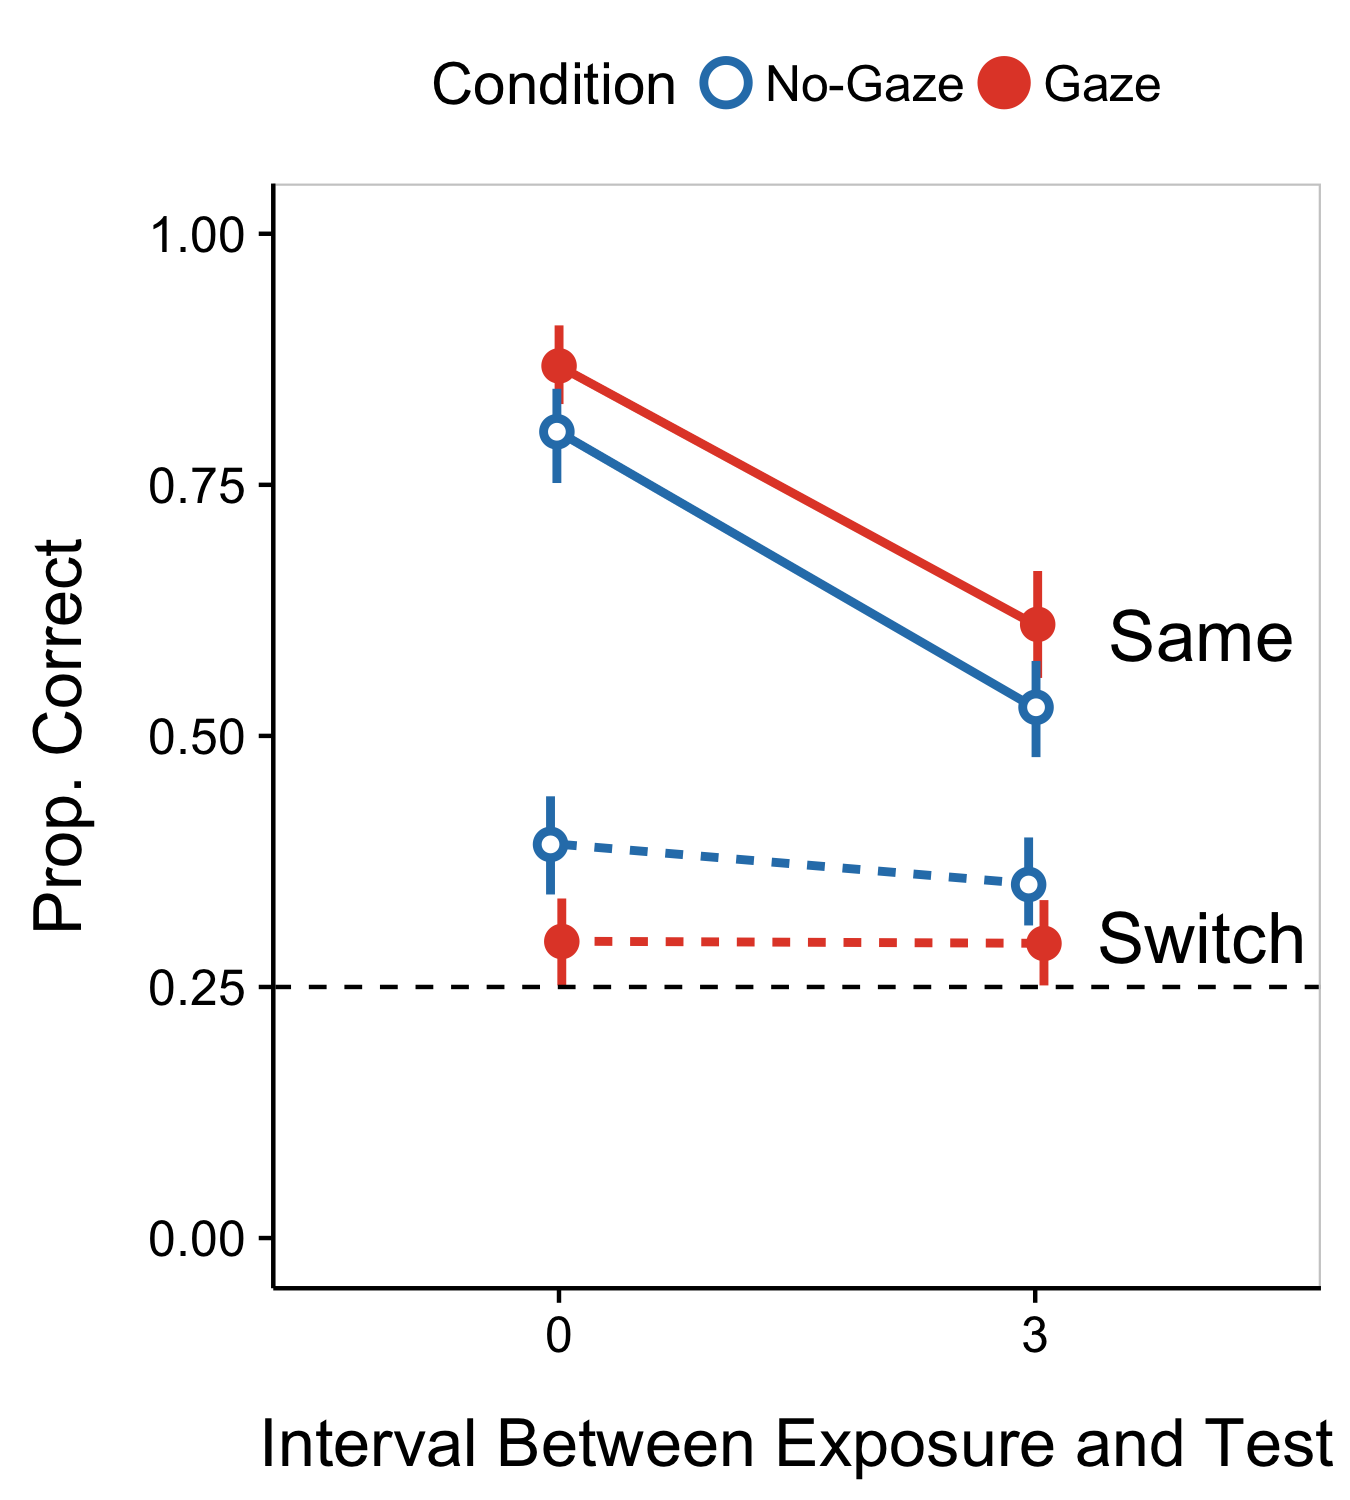
\includegraphics[width=0.5\linewidth]{/Users/ejyoon/Documents/Documents/Research/dissertation/index/chapter_child_rmds/SOC-XSIT/figures/expt4_collapsed} 

}

\caption[Experiment 4.4 results]{Experiment 4.4 results. Accuracy on test trials in Experiment 4 collapsed across the Long and Short inspection time conditions. The dashed line represents chance performance. Color and line type indicate whether there was gaze present on exposure trials. Error bars indicate 95\% confidence intervals computed by non-parametric bootstrap.}\label{fig:expt4-plot}
\end{figure}
We did not see strong evidence of an effect of the different inspection
times. Thus, all of the results reported here collapse across the short
and long inspection time conditions. For all analyses, we removed the
trials on which participants did not respond within the fixed inspection
time on exposure trials (0.05\% of trials).

\subsubsection{Exposure Trials}\label{exposure-trials-3}

Participants' responses on exposure trials differed from those expected
by chance (smallest \(\beta\) = 2.95, z = 38.08, \(p\) \textless{}
.001), suggesting that gaze was again effective in directing
participants' attention. Similar to Experiment 2, participants were
quite likely to use the gaze cue when it was a video of an actress
(\(M_{0-interval}\) = 0.93, \(M_{3-interval}\) = 0.95).

\subsubsection{Test Trials}\label{test-trials-3}

Figure 6 shows performance on test trials in Experiment 4. In the
majority of conditions, participants selected the correct referent at
rates greater than chance (smallest \(\beta\) = 0.2, z = 2.2, \(p\)
\textless{} .05). However, participants' responses were not different
from chance on Switch trials after exposure trials with gaze in the
3-interval condition (\(\beta\) = 0.17, \(p\) = 0.06).

We replicate the key finding from Experiments 1-3: after seeing exposure
trials with gaze, participants were less accurate on Switch trials
(\(\beta\) = 0.9, \(p\) \textless{} .001). Since inspection times were
fixed across the Gaze and No-Gaze conditions, this finding provides
evidence that the presence of a referential cue did more than just
reduce the amount of time participants' spent inspecting the potential
word-object links. In contrast to Experiments 2 and 3, visual inspection
of Figure 6 suggested that the referential cue provided a boost to
accuracy on Same trials. To assess the simple effect of gaze on trial
type, we computed pairwise contrasts using the \emph{lsmeans} package in
R with a Bonferroni correction for multiple comparisons (Lenth, 2016).
Accuracy was higher for Same trials in the Gaze condition (\(\beta\) =
0.49, \(p\) \textless{} .001), but lower for Switch trials (\(\beta\) =
-0.41, \(p\) \textless{} .001). The boost in accuracy on Same trials
differs from Experiments 2 and 3 and suggests that making inspection
times equivalent across conditions allowed the social cue to affect the
strength of learners' memory for their candidate hypothesis.

The results of Experiment 4 help to clarify the effect of gaze on memory
in our task, providing evidence that the presence of a referential cue
did more than just reduce participants' visual inspection time. Instead,
gaze reduced memory for alternative word-object links even when people
had the same opportunity to visually inspect and encode them. We also
found evidence of a boost for learners' memory of their candidate
hypothesis in the gaze condition, an effect that we saw at the higher
number of referents and the longer intervals in Experiment 1, but that
we did not see in Experiments 2 or 3. One explanation for this
difference is that in Experiment 4, since participants' use of gaze was
independent of the length of exposure trials, inspection times in the
gaze condition were longer compared to those in Experiments 1-3. Thus,
it could be that the combination of a gaze cue coupled with the
opportunity to continue attending to the gaze target led to a boost in
performance on Same trials relative to trials without gaze.

\section{General Discussion}\label{general-discussion}

Tracking cross-situational word-object statistics allows word learning
to proceed despite the presence of individually ambiguous naming events.
But models of cross-situational learning disagree about how much
information is actually stored in memory, and the input to statistical
learning mechanisms can vary along a continuum of referential
uncertainty from unambiguous naming instances to highly ambiguous
situations. In the current line of work, we explore the hypothesis that
these two factors are fundamentally linked to one another and to the
social context in which word learning occurs. Specifically, we ask how
cross-situational learning operates over social input that varies the
amount of ambiguity in the learning context.

Our results suggest that the representations underlying
cross-situational learning are quite flexible. In the absence of a
referential cue to word meaning, learners tended to store more
alternative word-object links. In contrast, when gaze was present
learners stored less information, showing behavior consistent with
tracking a single hypothesis (Experiments 1 and 2). Learners were also
sensitive to a parametric manipulation of the strength of the
referential cue, showing a graded increase in the tendency to use the
cue as reliability increased, which in turn resulted in a graded
decrease in memory for alternative word-object links (Experiment 3).
Finally, learners stored less information in the presence of gaze even
when they were shown the objects for the same amount of time (Experiment
4).

In Experiments 2 and 3 reduced memory for alternative hypotheses did not
result in a boost to memory for learners' candidate hypothesis. This
pattern of data suggests that the presence of a referential cue
selectively affected one component of the underlying representation: the
number of alternative word-object links, and not the strength of the
learners' candidate hypothesis. However, in Experiments 1 and 4, we did
see some evidence of stronger memory for learners' initial hypothesis in
the presence of gaze: at the higher number of referents and interval
conditions (Experiment 1), and when the length of exposure trials was
equivalent across the Gaze and No-Gaze conditions (Experiment 4). We
speculate that the relationship between the presence of a referential
cue and the strength of learners' candidate hypothesis is modulated by
how the cue interacts with attention. In Experiment 1, gaze may have
provided a boost because, in the absence of gaze, attention would have
been distributed across a larger number of alternatives. And, in
Experiment 4, gaze may have led to better memory because it was coupled
with the opportunity for sustained attention to the gaze target. More
work is needed in order to understand precisely when the presence of
gaze affects this particular component of the representations underlying
cross-situational learning.

In Experiments 1-3, longer inspection times (i.e., more time spent
encoding the word-object links during learning) led to better memory at
test. We did, however, find slightly different interaction effects
across our studies. In Experiment 1, longer inspection times led to
higher accuracy in the No-Gaze condition for both Same and Switch
trials. In Experiment 2, longer inspection times provided a larger boost
to performance on Switch trials compared to Same trials, regardless of
gaze condition. Despite these differences, we speculate that inspection
time played a similar role across these studies: When a social cue was
present, learners' attention was focused and inspection times tended to
be shorter, which led to worse performance on Switch trials (i.e.,
reduced memory for alternative word-object links). Interestingly, in
Experiment 4, we found an effect of social cues on memory for
alternatives even when participants were given the same opportunity to
visually inspect the objects, suggesting that gaze does more than just
modulate visual attention during learning.

\subsection{Relationship to previous
work}\label{relationship-to-previous-work}

Why might a decrease in memory for alternatives fail to increase the
strength of learners' memory for their candidate hypothesis? One
possibility is that participants did not shift their cognitive resources
from the set of alternatives to their single hypothesis, but instead
chose to use the gaze information to reduce inspection time, thus
conserving their resources for future use. Griffiths, Lieder, and
Goodman (2015) formalize this behavior by pushing the rationality of
computational-level models down to the psychological process level. In
their framework, cognitive systems are thought to be adaptive in that
they optimize the use of their limited resources, taking the cost of
computation (e.g., the opportunity cost of time or mental energy) into
account. For example, Vul, Goodman, Griffiths, and Tenenbaum (2014)
showed that as time pressure increased in a decision-making task,
participants were more likely to show behavior consistent with a less
cognitively challenging strategy of matching, rather than with the
globally optimal strategy. In the current work, we found that learners
showed evidence of altering how they allocated cognitive resources based
on the amount of referential uncertainty present during learning,
spending less time inspecting alternative word-object links and reducing
the number of links stored in memory when uncertainty was low.

Our results fit well with recent experimental work that investigates how
attention and memory can constrain infants' statistical word learning.
For example, Smith and Yu (2013) used a modified cross-situational
learning task to show that only infants who disengaged from a novel
object to look at both potential referents were able to learn the
correct word--object mappings. Moreover, Vlach and Johnson (2013) showed
that 16-month-olds were only able to learn from adjacent
cross-situational co-occurrence statistics, and unable to learn from
co-occurrences that were separated in time. Both of these findings make
the important point that only the information that comes into contact
with the learning system can be used for cross-situational word
learning, and this information is directly influenced by the attention
and memory constraints of the learner. These results also add to a large
literature showing the importance of social information for word
learning (P. Bloom, 2002; E. V. Clark, 2009) and to recent work
exploring the interaction between statistical learning mechanisms and
other types of information (Frank et al., 2009; Koehne \& Crocker, 2014;
Yu \& Ballard, 2007). Our findings suggest that referential cues affect
statistical learning by modulating the amount of information that
learners store in the underlying representations that support learning
over time.

Is gaze a privileged cue, or could other, less-social cues (e.g., an
arrow) also affect the representations underlying cross-situational
learning? On the one hand, previous research has shown that gaze cues
lead to more reflexive attentional responses compared to arrows
(Friesen, Ristic, \& Kingstone, 2004), that gaze-triggered attention
results in better learning compared to salience-triggered attention (R.
Wu \& Kirkham, 2010), and that even toddlers readily use gaze to infer
novel word meanings (D. A. Baldwin, 1993). Thus, it could be that gaze
is an especially effective cue for constraining word learning since it
communicates a speaker's referential intent and is a particularly good
way to guide attention. On the other hand, the generative process of the
cue -- whether it is more or less social in nature -- might be less
important; instead, the critical factor might be whether the cue
effectively reduces uncertainty in the naming event. Under this account,
gaze is placed amongst a set of many cues that could produce similar
effects as those reported here. Future work could explore a wider range
of cues to see if they modulate the representations underlying
cross-situational learning in a similar way.

How should we characterize the effect of gaze on attention and memory in
our task? One possibility is that the referential cue acts as a filter,
only allowing likely referents to contact statistical learning
mechanisms (Yu \& Ballard, 2007). This `filtering account' separates the
effect of social cues from the underlying computation that aggregates
cross-situational information. Another possibility is that referential
cues provide evidence about a speaker's communicative intent (Frank et
al., 2009). In this model, the learner is reasoning about the speaker
and word meanings simultaneously, which places inferences based on
social information as part of the underlying computation. A third
possibility is that participants thought of the referential cue as
pedagogical. In this context, learners assume that the speaker will
choose an action that is most likely to increase the learner's belief in
the true state of the world (Shafto et al., 2012b), making it
unnecessary to allocate resources to alternative hypotheses. Experiments
show that children spend less time exploring an object and are less
likely to discover alternative object-functions if a single function is
demonstrated in a pedagogical context (Bonawitz et al., 2011). However,
because the results from the current study cannot distinguish between
these explanations, these questions remain topics for future studies
specifically designed to tease apart these possibilities.

\subsection{Limitations}\label{limitations}

There are several limitations to the current study that are worth
noting. First, the social context that we used was relatively
impoverished. Although we moved beyond a simple manipulation of the
presence or absence of social information in Experiment 3, we
nevertheless isolated just a single cue to reference, gaze. But
real-world learning contexts are much more complex, providing learners
access to multiple cues such as gaze, pointing, and previous discourse.
In fact, Frank, Tenenbaum, and Fernald (2013) analyzed a corpus of
parent-child interactions and concluded that learners would do better to
aggregate noisy social information from multiple cues, rather than
monitor a single cue since no single cue was a consistent predictor of
reference. In our data, we did see a more reliable effect of referential
cues when we used a video of an actress, which included both gaze and
head turn as opposed to the static, schematic stimuli, which only
included gaze. It is still an open and interesting question as to how
our results would generalize to learning environments that contain a
rich combination of social cues.

Second, we do not yet know how variations in referential uncertainty
during learning would affect the representations of young word learners,
the age at which cross-situational word learning might be particularly
important. Recent research using a similar paradigm as our own did not
find evidence that 2- or 3-year-olds stored multiple word-object links;
instead, children only retained a single candidate hypothesis (Woodard,
Gleitman, \& Trueswell, 2016). However, performance limitations on
children's developing attention and memory systems (Colombo, 2001;
Ross-sheehy, Oakes, \& Luck, 2003) could make success on these explicit
response tasks more difficult. Moreover, our work suggests that
different levels of referential uncertainty in naturalistic learning
contexts (see Medina, Snedeker, Trueswell, \& Gleitman, 2011; Yurovsky
\& Frank, 2015) might evoke different strategies for information
storage, with learners retaining more information as ambiguity in the
input increases. Thus, we think that it will be important to test a
variety of outcome measures and learning contexts to see if younger
learners show evidence of storing multiple word meanings during
learning.

In addition, previous work with infants has shown that their attention
is often stimulus-driven and sticky (Oakes, 2011), suggesting that very
young word learners might not effectively explore the visual scene in
order to extract the necessary statistics for storing multiple
alternatives. It could be that referential cues play an even more
important role for young learners by filtering the input to
cross-situational word learning mechanisms and guiding children to the
relevant statistics in the input. In fact, recent work has shown that
the precise timing of features such as increased parent attention and
gesturing towards a named object and away from non-target objects were
strong predictors of referential clarity in a naming event (Trueswell et
al., 2016). It could be that the statistics available in these
particularly unambiguous naming events are the most useful for
cross-situational learning.

Finally, the current experiments used a restricted cross-situational
word learning scenario, which differs from real-world language learning
contexts in several important ways. One, we only tested a single
exposure for each novel word-object pairing; whereas, real-world naming
events are best characterized by discourse where an object is likely to
be named repeatedly in a short amount of time (Frank, Tenenbaum, \&
Fernald, 2013; Rohde \& Frank, 2014). Two, the restricted visual world
of 2-8 objects on a screen combined with the forced-choice response
format may have biased people to assume that all words in the task must
have referred to one of the objects. But, in actual language use, people
can refer to things that are not physically co-present (e.g., Gleitman,
1990), creating a scenario where learners would not benefit from storing
additional word-object links in the absence of clear referential cues.
Finally, we presented novel words in isolation, removing any sentential
cues to word meaning (e.g., verb-argument relations). In fact, previous
work with adults has shown that cross-situational learning mechanisms
only operate in contexts where sentence-level constraints do not
completely disambiguate meaning (Koehne \& Crocker, 2014). Thus, we need
more evidence to understand how the representations underlying
cross-situational learning change in response to referential uncertainty
at different timescales and in richer language contexts that more
accurately reflect real-world learning environments.

\section{Conclusions}\label{conclusions}

Word learning proceeds despite the potential for high levels of
referential uncertainty and despite learners' limited cognitive
resources. Our work shows that cross-situational learners flexibly
respond to the amount of ambiguity in the input, and as referential
uncertainty increases, learners tend to store more word-object links.
Overall, these results bring together aspects of social and statistical
accounts of word learning to increase our understanding of how
statistical learning mechanisms operate over fundamentally social input.

\chapter{Integrating statistical and social information during language
comprehension and word
learning}\label{integrating-statistical-and-social-information-during-language-comprehension-and-word-learning}

\chaptermark{Seeking social information during language processing}

In this chapter, I present three studies that explore how the presence
of a social cue to reference (a speaker's gaze) changes listeners'
decisions about visual fixation during language comprehension and word
learning. Within our broader active-social framework, these studies ask
how the value of information gained from fixating on (i.e., querying) a
social partner interacts with learners' developing knowledge of word
meanings (i.e., hypotheses) to modulate their information accumulation
thresholds (i.e., stopping rules). This work brings together the core
elements -- active, social, and statistical -- of the integrative
account described in Chapter 1.

Children process language in complex environments where there are often
many things to talk about. How do they understand and learn words
despite this noisy input? Statistical learning accounts emphasize that
children can aggregate consistent word-object co-occurrences across
multiple labeling events to reduce uncertainty over time.
Social-pragmatic theories argue that interactions with social partners
support learning by reducing ambiguity within individual labeling
events. Here, we present three eye-tracking studies that ask how
children integrate statistical and social information during real-time
language processing. First, children and adults did not delay their gaze
shifts to gather a post-nominal social cue to reference (another
speaker's eye gaze). Second, when processing novel words, adults fixated
more on a speaker who provided a disambiguating gaze and showed stronger
recall for word-object links learned via the social cue. Finally, in
contrast to the familiar word context, children and adults fixated
longer on a speaker who produced a gaze cue when labeling novel objects,
which, in turn, led to increased looking to the named object and less
looking to the other objects in the scene. Moreover, children, but not
adults, increased their looking to the interlocutor throughout the
experiment. Together, these results suggest that learners flexibly
integrate their knowledge of object labels to decide whether to seek
social information, which then shapes the information that comes into
contact with statistical learning mechanisms.

\chapter*{Conclusion}\label{conclusion}
\addcontentsline{toc}{chapter}{Conclusion}

In this dissertation, I proposed a framework for understanding
children's information-seeking decisions within social contexts. The
core of the argument is that the presence of other people can change the
\emph{availability} and \emph{usefulness} of information-seeking
behaviors by shaping learners' goals, hypotheses, actions, answers, and
thresholds for stopping information gathering. Following the theoretical
framework, I presented a set of empirical studies that explored whether
the dynamics of children's real-time information selection via their eye
movements flexibly adapts to gather social information that supports
language processing.

Chapter 2 investigated how children learning American Sign Language
(ASL) distributed visual attention between the linguistic signal and
referents, which both compete for visual attention. Similar to children
learning spoken language, ASL learners shifted gaze away from a social
partner to seek objects before sign offset, providing evidence that,
despite channel competition, language drove rapid shifts in visual
attention to named referents. Chapter 3 extended the sign language
research by directly comparing ASL learners' gaze dynamics to those of
children learning spoken English using parallel real-time language
comprehension tasks. Chapter 3 also presented a comparison of
English-learning children and adults' eye movements in noisy vs.~clear
auditory contexts. In both the ASL and noisy speech cases, listeners
adapted their gaze to seek additional language-relevant information from
social partners before shifting to seek a named referent. Chapters 4 and
5 explored how eye movements change when children and adults processed
familiar and novel words accompanied by social cues to reference. Taken
together, the social gaze work suggests that children integrate their
uncertainty over word-object mappings to decide when to seek social
information, which in turn, modulates the input to statistical word
learning.

The integrative framework and empirical work described here are limited
in several important ways. First, the majority of this research tested
binary hypotheses of behavior change -- i.e., sign vs.~spoken language;
noisy vs.~clear speech; word learning with vs.~without social gaze -- to
answer the question of whether children would flexibly adapt their
information seeking in response to changes in their processing
environments. Chapters 2-5 present evidence across a diverse set of case
studies that children's real-time information seeking is quite flexible.
However, to move the integrative framework forward, we would want to
develop a fully-specified model that could make quantitative predictions
about how social contexts will change the utility of information-seeking
behaviors. This step will require formalizing the notions of value and
cost of information-seeking actions in a modeling framework that can
incorporate the effects of reasoning about other people's mental states.

We have taken some initial steps towards this goal by developing a model
of active-social learning that integrates ideas from Optimal Experiment
Design (OED) with formalizations of recursive social reasoning from
Bayesian models of pragmatic language interpretation (Goodman \& Frank,
2016). We found that this integrated model was able to reproduce the
qualitative patterns in adults' decisions of whether to forego
information seeking in favor of more immediately rewarding actions when
their social partner highlighted performance and presentational goals
(E. J. Yoon et al., 2018). The integrative framework described here
directly inspired this line of research, and I hope that future versions
of the model will be able to generate graded, testable predictions for
behavior across a variety of domains -- e.g., eye movements, early
vocalizations, and verbal question asking.

Second, we used one particular formalization of active inquiry. The OED
model focuses on learners' information-seeking decisions given a
specific goal to learn and a set of candidate hypotheses. Other
computational frameworks have formalized active learning in different
ways. For example, foraging models pursue the analogy that human
information seeking is similar to animals' decisions about where and how
long to look for food if they were trying to maximize caloric intake
while minimizing their effort and time (see Pirolli \& Card (1999) for a
review). Cognitive scientists have successfully modeled a range of
behaviors as a form of spatial foraging, such as searching for semantic
concepts in memory (Hills et al., 2012) and decisions about where to
direct visual attention in real-time (Manohar \& Husain, 2013). In
addition to these search models, recent work on curiosity-based learning
in developmental robotics has created algorithms that optimize intrinsic
estimates of learning progress. This formalization creates systems that
focus on seeking activities and stimuli of intermediate complexity where
learners' predictions are steadily improving, and uncertainty is
steadily decreasing (Oudeyer \& Smith, 2016). One of the challenges for
researchers trying to integrate active and social learning is that the
space of possible connections is quite large. By constraining our
framework to active decision making, we were able to make some progress
on an important sub-component of a larger set of children's
information-seeking behaviors. Future theoretical work, however, should
consider possible connections between social learning phenomena and the
foraging/curiosity-based learning frameworks.

Third, our ultimate goal for the active-social framework is to
incorporate effects at a developmental timescale. The experiments in
this thesis, however, often treated children and adults as two endpoints
on a continuum, exploring parallels and differences between children's
information seeking and our best estimate of the mature state of the
language processing system. We did find some clear patterns of
developmental change. In Chapter 3, adults were faster to respond to
familiar words, generated more language-consistent shifts, and produced
fewer early shifts before accumulating enough information. Older
children were also faster to respond than younger children but did not
generate more language-consistent shifts overall. Older children did,
however, produce fewer early, non-language-driven gaze shifts. This
pattern of results suggests that what might be developing is an ability
to inhibit a behavior -- shifting gaze away from the language source --
that reduces access to information that is useful for figuring out the
identity of a named referent. Prior work also shows that children
develop greater flexibility in ignoring irrelevant information to focus
on parts of the meaningful parts of a sentence (Zangl \& Fernald, 2007).
But it is still an open question as to how children's visual information
seeking might change as they become more efficient in processing words
and develop their skill in focusing on relevant information in their
environment.

In addition to change at the developmental timescale, the final
experiment in Chapter 5 represents an exception where we measured
adaptation of information seeking over the slightly longer timescale of
multiple exposures to novel word-object links and in the context of
highly familiar words, which children learned through exposure to many
prior labeling events in their day-to-day lives. While the study in
Chapter 5 is a useful first step, future work should measure change over
a longer timescale by densely sampling children at different ages and
points of development. For example, it would be useful to know the
effect of children's rapidly improving productive language skills, which
increases the set of information-seeking actions available by allowing
children to ask verbal questions. One prediction based on our framework
is that seeking social information via eye movements should become less
useful when children can produce the verbal question ``What is this
thing called?'' since it has a higher probability of returning useful
information. Another example is children's rapid theory of mind
development. Our framework predicts that young children should focus
more on learning goals if they are less skilled at reasoning about
others' beliefs. But, as their social reasoning abilities mature and
their social environments become more complex, children may forego
information seeking actions that make them appear incompetent to their
social partners.

Fourth, our account is currently underdeveloped concerning individual
differences. That is, the model was designed to explore general
principles about how qualitative changes to the social environment might
shape children's information seeking actions. However, it is possible to
use the active-social framework to understand how individual differences
in children's input and cognitive abilities might interact to shape how
they decide to seek information from social partners. For example, prior
research has found that adults vary in the proportion of unambiguous
naming episodes they provide, with some parents rarely providing highly
informative contexts and others' doing so relatively more often
(Cartmill et al., 2013). Within our active-social framework, this
differential experience could be instantiated as children learning a
model of the probability of getting a high-quality answer when they ask
a question. If children do not expect an answer is likely, then this
should reduce information seeking even if there is a social partner
available. We did find some evidence of this effect in Chapters 4 and 5
where adults were less likely to use an unreliable social cue to
reference and where children looked more to a social partner who
provided gaze cue than to one who did not.

Individual differences in cognitive abilities could also be included in
our model. Prior research shows variability in children's theory of mind
and inhibitory control abilities (Carlson \& Moses, 2001), in addition
to the considerable variability in language processing skill (Marchman
\& Fernald, 2008). Within our active-social framework, children with a
more-developed theory of mind skill might place a higher weight on
pursuing social goals over and above informational goals, taking actions
that maintain others' beliefs about their abilities. It could also be
that stronger perspective-taking skills help children reason about the
probability of getting a quality answer from another person, thus
modulating whom they choose to ask questions (e.g., seeking information
from an expert vs.~a novice). Another compelling possibility is that
children who have stronger domain-general processing abilities are
better able to update their beliefs based on the information they
receive, and thus reducing the amount of time they spend seeking
information from social partners. These are all interesting, open
questions for future research that fall out of the integrative
active-social framework proposed in this thesis.

Finally, the empirical research described here aimed to understand how
children's information-seeking behaviors adapt to support their language
processing. To accomplish this, we measured changes in children's gaze
dynamics during language comprehension and word learning in simplified
environments. This approach has the benefit of providing a high degree
of experimenter control and a relatively well-understood hypothesis
linking observable behavior (eye movements) to underlying psychological
constructs (e.g., lexical access) (Tanenhaus, Magnuson, Dahan, \&
Chambers, 2000). The risk, however, is that the responses that we can
measure in the lab do not reflect behaviors that support children's
learning in their natural environments. That is, children acquire their
first language from conversations where social partners produce
contingent responses and take actions that control the flow of
children's learning experience. This gap suggests two critical next
steps for the research described here: (1) measure changes in children's
information seeking within free-flowing social interactions with their
caregivers (see Franchak, Kretch, \& Adolph (2018) for a recent example
of this approach using head-mounted eye trackers), and (2) develop more
realistic lab-based experiments that incorporate behaviorally-relevant
features of children's learning environments such as contingent
responding to children's actions (see Benitez \& Saffran (2018) for an
example of studying word learning using a gaze-contingent eye-tracking
paradigm).

In sum, we set out to explore how children's eye movements adapt to a
wide range of social contexts during two ecologically-relevant tasks:
familiar language comprehension and novel word learning. We found that
children could adapt their gaze to seek relevant social information when
it was useful for language processing. Moreover, children and adults
showed evidence of differential learning of new words when social gaze
guided their visual attention. This work highlighted two critical, open
challenges for a framework of information-seeking within social
contexts: (1) develop a precise quantitative model of how social
learning can change the utility of information-seeking behaviors, and
(2) move beyond highly-constrained lab experiments to document
information seeking behaviors in children's natural learning
environments. Despite these challenges, the integrative framework
presented in this thesis represents a way forward for understanding how
children's information seeking adapts to the wide variety of social
environments in which children acquire their first language.

\appendix

\chapter{Supplementary materials for Chapter
1}\label{supplementary-materials-for-chapter-1}

\section{Mathematical details of Optimal Experiment
Design}\label{mathematical-details-of-optimal-experiment-design}

This supplement contains the mathematical details of the OED approach as
described in Coenen et al. (2017). The goal is to provide a concrete
foundation for the conceptual analysis of how social learning contexts
can influence different components of active learning.

The OED model quantifies the \emph{expected utility} of different
information seeking actions. Formally, the set of queries is defined as
\(Q_1, Q_2,..., Q_n = \{Q\}\). The expected utility of each query
(\(EU(Q)\)) is a function of two factors: (1) the probability of
obtaining a specific answer \(P(a)\) weighted by (2) the usefulness of
that answer for achieving the learning goal \(U(a)\).

\[EU(Q) = \sum_{a\in q}{P(a)U(a)}\] \noindent
There are a variety of ways to define the usefulness function to score
each answer. An exhaustive review is beyond the scope of this paper (for
a detailed analysis of different approaches, see Nelson (2005)). One
standard method is to use \emph{information gain}, which is defined as
the change in the learner's overall uncertainty (difference in entoropy)
before and after receiving an answer.

\[U(a) = ent(H) - ent(H|a)\]

\noindent
Where \(ent(H)\) is defined using Shannon entropy\footnote{Shannon
  entropy is a measure of unpredictability or amount of uncertainty in
  the learner's probability distribution over hypotheses. Intuitively,
  higher entropy distributions are more uncertain and harder to predict.
  For example, if the learner believes that all hypotheses are equally
  likely, then they are in a state of high uncertainty/entropy. In
  contrast, if the learner firmly believes in one hypothesis, then
  uncertainty/entropy is low.} (MacKay, 2003), which provides a measure
of the overall amount of uncertainty in the learner's beliefs about the
candidate hypotheses.

\[ent(H) = -\sum_{a\in A}{P(h)log_2P(h)}\] \noindent
The conditional entropy computation is the same, but takes into account
the change in the learner's beliefs after seeing an answer.

\[ ent(H|a) = -\sum_{h\in H}{P(h|a)logP(h|a)} \] \noindent
To calculate the change in the learner's belief in a hypothesis
\(P(h|a)\), we use Bayes rule.

\[ P(h|a) = \frac{P(h)P(a|h)}{P(a)} \]

\noindent
If the researcher defines all these parts of the OED model (hypotheses,
questions, answers, and the usefulness function), then selecting the
optimal query is straightforward. The learner performs the expected
utility computation for each query in the set of possible queries and
picks the one that maximizes utility. In practice, the learner considers
each possible answer, scores the answer with the usefulness function,
and weights the score using the probability of getting that answer.

Before reviewing the behavioral evidence for OED-like reasoning in
adults and children, I will present a worked example of how to compute
the expected utility of a single query. The goal is to provide simple
calculations that illustrate how reasoning about hypotheses, questions,
and answers can lead to selecting useful actions. This example is
slightly modified from Nelson (2005).

Imagine that you are a biologist, and you come across a new animal that
you think belongs to one of two species: ``glom'' or ``fizo.'' You
cannot directly query the category identity, but you can gather
information about the presence or absence of two features (eats meat? or
is nocturnal?) that you know from prior research are more or less likely
for each of the species. The following probabilities summarise this
prior knowledge:
\begin{itemize}
\tightlist
\item
  \(P(eatsMeat \mid glom) = 0.1\)\\
\item
  \(P(eatsMeat \mid fizo) = 0.9\)
\item
  \(P(nocturnal \mid glom) = 0.3\)\\
\item
  \(P(nocturnal \mid fizo) = 0.5\)
\end{itemize}
\noindent   You also know from previous research that the probability of
seeing a glom or a fizo in the wild is:
\begin{itemize}
\tightlist
\item
  \(P(glom) = 0.7\)
\item
  \(P(fizo) = 0.3\)
\end{itemize}
\noindent   Which feature should you test: eats meat? or sleeps at
night? Intuitively, it seems better to test whether the creature eats
meat because an answer to this question provides good evidence about
whether the animal is a fizo since \(P(eatsMeat \mid fizo) = 0.9\).
However, the OED computation allows the biologist to go beyond this
intuition and compute precisely how much better it is to ask the ``eats
meat?'' question. All the scientist has to do is pass her knowledge
about the hypotheses and features through the expected utility
computation.

Here are the steps of the OED computation for calculating the utility of
the ``eats meat?'' question. First, we use Bayes rule to calculate how
much our beliefs would change if we received a ``yes'' or a ``no''
answer.\footnote{Note that the \(P(eatsMeat)\) term is computed by
  taking
  \(P(eatsMeat) = [P(eatsMeat \mid glom) \ times P(glom)] + [P(eatsMeat \mid fizo) \times P(fizo)] = (0.1 \times 0.7) + (0.9 \times 0.3) = 0.34\)}

\[ P(glom \mid eatsMeat) = \frac{P(eatsMeat \mid glom) \times P(glom)}{P(eatsMeat)} = \frac{0.1 \times 0.7}{0.34} = 0.21 \]

\noindent
Next, we calculate the uncertainty over the Species hypothesis before
doing any experiment. We do this by computing the prior entropy.

\[
\begin{aligned}
ent(Species) &= -\sum_{h\in H}{P(h) \times log_2P(h)} \\
 &= [-P(glom) \times log_2P(glom)]+[-P(fizo) \times log_2P(fizo)]\\
 &= [-(0.7 \times log_2(0.7)] + [-(0.3 \times log_2(0.3)]\\
 &= 0.88
\end{aligned}
\]

\noindent
To calculate information gain, we also need to compute our uncertainty
over hypotheses conditional on seeing each answer, or the posterior
entropy. First, for the ``yes'' answer:

\[
\begin{aligned}
ent(Species|eatsMeat = yes) &= -\sum_{a\in A}P(Species \mid eatsMeat = yes) \times log_2P(species \mid eatsMeat = yes) \\
&= [0.21 \times log_2(0.21)] + [0.79 \times log_2(0.79)]\\
&=  0.73
\end{aligned}
\]

\noindent
We use the difference between the prior and posterior entropy to compute
the utility of the ``yes'' answer.

\[
\begin{aligned}
U(a = yes) &= ent(Species) - ent(Species \mid eatsMeat = yes)\\
&= 0.88 - 0.73 \\
&= 0.15
\end{aligned}
\]

\noindent
Next, we do the same process for the ``no'' answer. First, we calculate
the posterior entropy.

\[ 
\begin{aligned}
ent(Species|eatsMeat = no) &= -\sum_{a\in A}{P(Species \mid eatsMeat = no) \times log_2P(species \mid eatsMeat = no)}\\
&= [0.95 \times log_2(0.95)] + [0.05 \times log_2(0.05)]\\
&=  0.27
\end{aligned}
\]

\noindent
Again, we use the difference between the prior and posterior entropy to
compute the utility of the ``no'' answer.

\[ 
\begin{aligned}
U(a = no) &= ent(Species) - ent(Species \mid eatsMeat = no)\\
&= 0.88 - 0.27 \\
&= 0.61
\end{aligned}
\]

\noindent
Note that the \(U(a = no) > U(a = yes)\). This captures the intuition
that learning that the animal does not eat meat would provide strong
evidence against the ``fizo'' hypothesis since
\(P(eatsMeat \mid fizo) = 0.9\). Finally, to compute the overall
expected information gain for the \textbf{``eats meat?'' question}, we
weight the utility of each answer by its probability:

\[
\begin{aligned}
EU(Q = eatsMeat) &= \sum_{a\in A}{P(a)U(a)} \\
&= [P(eatsMeat = yes) \times U(eatsMeat = yes)] + \\& \qquad \qquad \qquad [P(eatsMeat = no) \times U(eatsMeat = no)]\\
&= [0.34 \times 0.15] + [0.66 \times 0.61]\\
&= 0.46
\end{aligned}
\]

If we performed the same steps to calculate the expected utility of the
``sleeps at night?'' question, we get \(EU(Q = sleepsNight) = 0.026\).
So if the biologist wants to maximize the chance of gaining useful
information, she should select the ``eats meat?'' experiment since
\(EU(Q = eatsMeat) > EU(Q = sleepsNight)\).

\chapter{Supplementary materials for Chapter
2}\label{supplementary-materials-for-chapter-2}

In this appendix, we present four pieces of supplemental information.
First, we provide details about the Bayesian models used to analyze the
data. Second, we present a sensitivity analysis that provides evidence
that the estimates of the associations between age/vocabulary and
accuracy/reaction time (RT) are robust to different parameterizations of
the prior distribution and different cutoffs for the analysis window.
Third, we present the results of a parallel set of analyses using a
non-Bayesian approach to show that these results are consistent
regardless of choice of analytic framework. And fourth, we present two
exploratory analyses measuring the effects of phonological overlap and
iconicity on RT and accuracy. In both analyses, we did not see evidence
that these factors changed the dynamics of eye movements during ASL
processing

\section{Model Specifications}\label{model-specifications}

Our key analyses use Bayesian linear models to test our hypotheses of
interest and to estimate the associations between age/vocabulary and
RT/accuracy. Figure S1 (Accuracy) and S2 (RT) present graphical models
that represent all of the data, parameters, and other variables of
interest, and their dependencies. Latent parameters are shown as
unshaded nodes while observed parameters and data are shown as shaded
nodes. All models were fit using JAGS software (Plummer, 2003) and
adapted from models in Kruschke (2014) and Lee and Wagenmakers (2014).

\subsection{Accuracy}\label{accuracy}
\begin{figure}[t]

{\centering 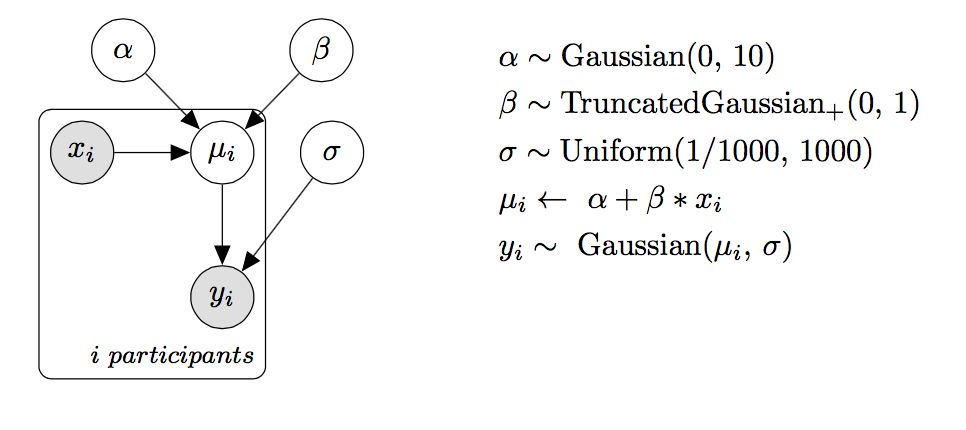
\includegraphics[width=0.75\linewidth]{/Users/ejyoon/Documents/Documents/Research/dissertation/index/chapter_child_rmds/SOL/figures/acc_model} 

}

\caption[Graphical representation of the accuracy model in Experiment 1.1.]{Graphical model representation of the linear regression used to predict accuracy. The shaded nodes represent observed data (i.e., each participant's age, vocabulary, and mean accuracy). Unshaded nodes represent latent parameters (i.e., the intercept and slope of the linear model).}\label{fig:unnamed-chunk-6}
\end{figure}
To test the association between age/vocabulary and accuracy we assume
each participant's mean accuracy is drawn from a Gaussian distribution
with a mean, \(\mu\), and a standard deviation, \(\sigma\). The mean is
a linear function of the intercept, \(\alpha\), which encodes the
expected value of the outcome variable when the predictor is zero, and
the slope, \(\beta\), which encodes the expected change in the outcome
with each unit change in the predictor (i.e., the strength of
association).

For \(\alpha\) and \(\sigma\), we use vague priors on a standardized
scale, allowing the model to consider a wide range of plausible values.
Since the slope parameter \(\beta\) is critical to our hypothesis of a
linear association, we chose to use an informed prior: that is, a
truncated Gaussian distribution with a mean of zero and a standard
deviation of one on a standardized scale. Centering the distribution at
zero is conservative and places the highest prior probability on a null
association, to reduce the chance that our model overfits the data.
Truncating the prior encodes our directional hypothesis that accuracy
should increase with age and larger vocabulary size. And using a
standard deviation of one constrains the plausible slope values, thus
making our alternative hypothesis more precise. We constrained the slope
values based on previous research with children learning spoken language
showing that the average gain in accuracy for one month of development
between 18-24 months to be \textasciitilde{}1.5\% (Fernald, Zangl,
Portillo, \& Marchman, 2008).

\subsection{Reaction Time}\label{reaction-time}
\begin{figure}[t]

{\centering 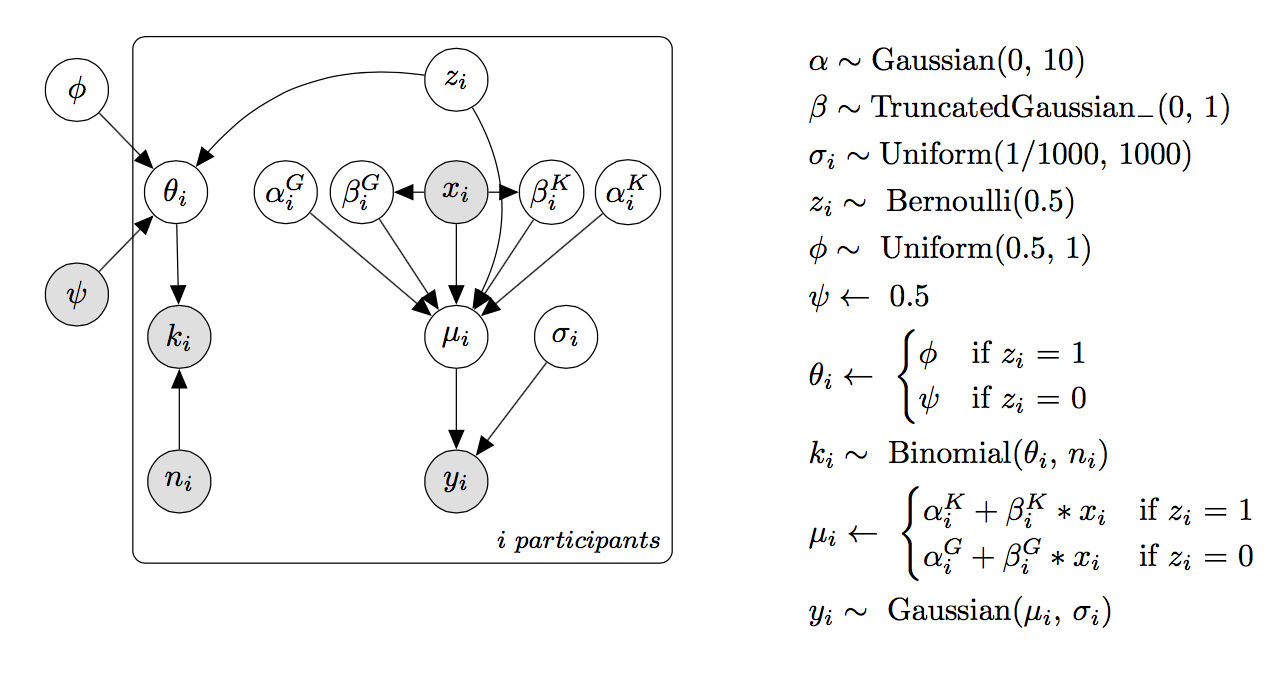
\includegraphics[width=0.75\linewidth]{/Users/ejyoon/Documents/Documents/Research/dissertation/index/chapter_child_rmds/SOL/figures/rt_model} 

}

\caption[Graphical representation of the RT model in Experiment 1.1.]{Graphical model representation of the linear regression plus latent mixture model (i.e., guessing model). The model assumes that each individual participant's first shift is either the result of guessing or knowledge. And the latent indicator $z_i$ determines whether that participant is included in the linear regression estimating the association between age/vocabulary and RT.}\label{fig:unnamed-chunk-7}
\end{figure}
The use of RT as a processing measure is based on the assumption that
the timing of a child's first shift reflects the speed of their
incremental language comprehension. Yet, some children have a first
shift that seems to be unassociated with this construct: their first
shift behavior appears random. We quantify this possibility for each
participant explicitly (i.e., the probability that the participant is a
``guesser'') and we create an analysis model where participants who were
more likely to be guessers have less of an influence on the estimated
relations between RT and age/vocabulary.

To quantify each participant's probability of guessing, we computed the
proportion of signer-to-target (correct) and signer-to-distracter
(incorrect) shifts for each child. We then used a latent mixture model
in which we assumed that the observed data, k\_i, were generated by two
processes (guessing and knowledge) that had different overall
probabilities of success, with the ``guessing group'' having a
probability of 50\%, \(\psi\), and the ``knowledge'' group having a
probability greater than 50\%, \(\phi\). The group membership of each
participant is a latent indicator variable, \(z_i\), inferred based on
that participant's proportion of correct signer-to-target shifts
relative to the overall proportion of correct shifts across all
participants (see Lee \& Wagenmakers (2014) for a detailed discussion of
this modeling approach). We then used each participant's inferred group
membership to determine whether they were included in the linear
regression. In sum, the model allows participants to contribute to the
estimated associations between age/vocabulary and RT proportional to our
belief that they were guessing.

As in the Accuracy model, we use vague priors for \(\alpha\) and
\(\sigma\) on a standardized scale. We again use an informed prior for
\(\beta\), making our alternative hypothesis more precise. That is, we
constrained the plausible slope values based on previous research with
children learning spoken language showing that the average gain in RT
for one month of development between 18-24 months to be
\textasciitilde{}30 ms (Fernald, Zangl, Portillo, \& Marchman, 2008).

\section{Sensitivity Analysis: Prior Distribution and Window
Selection}\label{sensitivity-analysis-prior-distribution-and-window-selection}
\begin{figure}[t]

{\centering 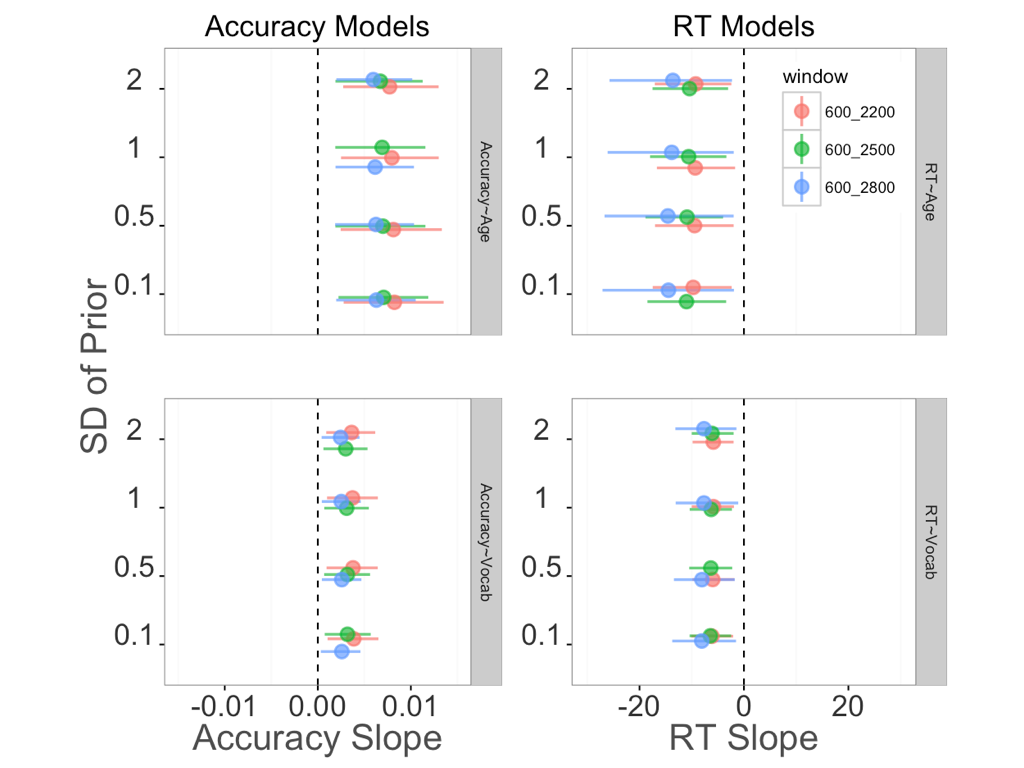
\includegraphics[width=0.75\linewidth]{/Users/ejyoon/Documents/Documents/Research/dissertation/index/chapter_child_rmds/SOL/figures/supp_coef_plot} 

}

\caption[Results of sensitivity analysis for Experiment 1.1.]{Coefficient plot for the slope parameter for four different parameterizations of the prior and for three different analysis windows. Each panel shows a different model. Each point represents a coefficient measuring the strength of association between the two variables. Error bars are 95\% HDIs around the coefficient. Color represents the three different analysis windows.}\label{fig:unnamed-chunk-8}
\end{figure}
We conducted a sensitivity analysis to show that our parameter estimates
for the associations between accuracy/RT and age/vocabulary are robust
to decisions about (a) the analysis window and (b) the specification of
the prior distribution on the slope parameter. Specifically, we varied
the parameterization of the standard deviation on the slope, allowing
the model to consider a wider or narrower range of values to be
plausible a priori. We also fit these different models to two additional
analysis windows +/- 300 ms from the final analysis window: 600-2500 ms
(the middle 90\% of the RT distribution in our experiment).
\begin{table}

\caption[Results for sensitivity analysis for Experiment 1.1]{\label{tab:unnamed-chunk-9}Bayes Factors for all four linear models fit to three different analysis windows using four different parameterizations of the prior distribution for the slope parameter.}
\centering
\resizebox{\linewidth}{!}{
\begin{tabular}[t]{>{\raggedright\arraybackslash}p{3.5cm}>{\raggedleft\arraybackslash}p{3cm}rrrr}
\toprule
\textbf{Analysis window} & \textbf{SD Slope} & \textbf{Acc\textasciitilde{}Age} & \textbf{Acc\textasciitilde{}Vocab} & \textbf{RT\textasciitilde{}Age} & \textbf{RT\textasciitilde{}Vocab}\\
\midrule
600 – 2200 ms & 3.2 & 6.2 & 3.7 & 2.4 & 4.1\\
NA & 1.4 & 14.1 & 5.5 & 3.5 & 8.6\\
NA & 1.0 & 19.4 & 8.9 & 5.0 & 9.2\\
NA & 0.7 & 22.7 & 11.6 & 7.8 & 17.0\\
600 – 2500 ms & 3.2 & 11.0 & 2.3 & 5.6 & 6.1\\
\addlinespace
NA & 1.4 & 9.7 & 4.0 & 13.8 & 10.5\\
NA & 1.0 & 12.8 & 6.8 & 12.5 & 18.2\\
NA & 0.7 & 15.6 & 6.8 & 17.9 & 20.7\\
600 – 2800 ms & 3.2 & 6.0 & 1.1 & 1.2 & 1.4\\
NA & 1.4 & 10.7 & 2.6 & 3.5 & 4.7\\
\addlinespace
NA & 1.0 & 13.5 & 4.0 & 3.7 & 4.0\\
NA & 0.7 & 15.2 & 4.6 & 5.5 & 5.6\\
\bottomrule
\end{tabular}}
\end{table}
Figure S3 shows the results of the sensitivity analysis, plotting the
coefficient for the \(\beta\) parameter in each model for the three
different analysis windows for each specification of the prior. All
models show similar coefficient values, suggesting that inferences about
the parameters are not sensitive to the exact form of the priors. Table
S1 shows the Bayes Factors for all models across three analysis windows
and fit using four different vales for the slope prior. The Bayes Factor
only drops below 3 when the prior distribution is quite broad (standard
deviation of 3.2) and only for the longest analysis window (600-2800
ms). In sum, the strength of evidence for a linear association is robust
to the choice of analysis window and prior specification.

\section{Parallel set of non-Bayesian
analyses}\label{parallel-set-of-non-bayesian-analyses}

First, we compare Accuracy and RT of native hearing and deaf signers
using a Welch Two Sample t-test and do not find evidence that these
groups are different (Accuracy: t(28) = 0.75, p = 0.45, 95\% CI on the
difference in means {[}-0.07, 0.14{]}; RT: t(28) = 0.75, p = 0.46, 95\%
CI on the difference in means {[}-125.47 ms, 264.99 ms{]}.

Second, we test whether children and adults tend to generate saccades
away from the central signer prior to the offset of the target sign. To
do this, we use a One Sample t-test with a null hypothesis that the true
mean is not equal to 1, and we find evidence against this null
(Children: M = 0.88, t(28) = -2.92, p = 0.007, 95\% CI {[}0.79, 0.96{]};
Adults: M = 0.51, t(15) = -6.87, p \textless{} 0.001, 95\% CI {[}0.35,
0.65{]})

Third, we fit the four linear models using MLE to estimate the relations
between the processing measures on the VLP task (Accuracy/RT) and
age/vocabulary. We follow recommendations from Barr (2008) and use a
logistic transform to convert the proportion accuracy scores to a scale
more suitable for the linear model.
\begin{table}

\caption[Results for MLE models fit to data in Experiment 1.1.]{\label{tab:unnamed-chunk-10}Results for the four linear models fit using Maxiumum Likelihood Estimation. All p-values are one-sided to reflect our directional hypotheses about the VLP measures improving over development.}
\centering
\resizebox{\linewidth}{!}{
\begin{tabular}[t]{>{\raggedright\arraybackslash}p{3.5cm}>{\raggedleft\arraybackslash}p{3cm}rrr}
\toprule
\textbf{Model specification} & \textbf{Mean Beta value} & \textbf{std. error} & \textbf{t-statistic} & \textbf{p-value}\\
\midrule
logit(accuracy) \textasciitilde{} age + hearing status & 0.003 & 0.012 & 2.59 & 0.008\\
logit(accuracy) \textasciitilde{} vocabulary + hearing status & 0.002 & 0.006 & 2.27 & 0.015\\
RT \textasciitilde{} age + hearing status & -10.050 & 4.620 & -2.17 & 0.019\\
RT \textasciitilde{} vocabulary + hearing status & -6.340 & 2.180 & -2.91 & 0.003\\
\bottomrule
\end{tabular}}
\end{table}
\section{Analyses of phonological overlap and
iconicity}\label{analyses-of-phonological-overlap-and-iconicity}
\begin{figure}[t]

{\centering 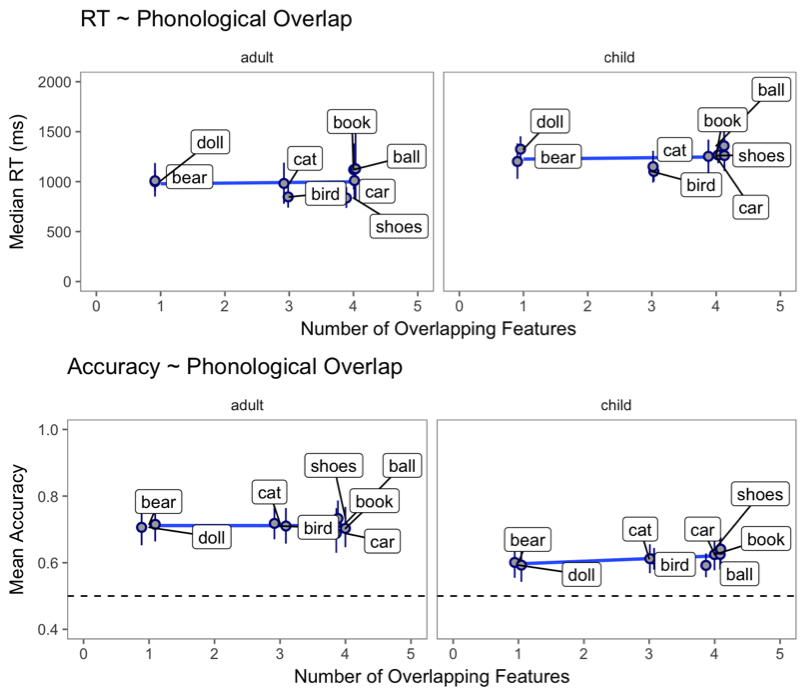
\includegraphics[width=0.75\linewidth]{/Users/ejyoon/Documents/Documents/Research/dissertation/index/chapter_child_rmds/SOL/figures/phonological_overlap} 

}

\caption[Association between degree of phonological overlap and RT/Accuracy in Experiment 1.1.]{Scatterplot of the association between degree of phonological overlap and RT (top row) and accuracy (bottom row) for both adults (left column) and children (right column). The blue line represents a linear model fit.}\label{fig:unnamed-chunk-11}
\end{figure}
First, we analyzed whether phonological overlap of our item-pairs might
have influenced adults and children's RTs and accuracy. Signs that are
higher in phonological overlap might have been more difficult to process
because they are more confusable. Here, phonological overlap is
quantified as the number of features (e.g., Selected Fingers, Major
Location, Movement, Sign Type) that both signs shared. Values were taken
from a recently created database (ASL-LEX) of lexical and phonological
properties of nearly 1,000 signs of American Sign Language (Caselli et
al., 2017). Our item-pairs varied in degree of overlap from 1-4
features. We did not see evidence that degree of phonological overlap
influenced either processing measure in the VLP task.
\begin{figure}[t]

{\centering 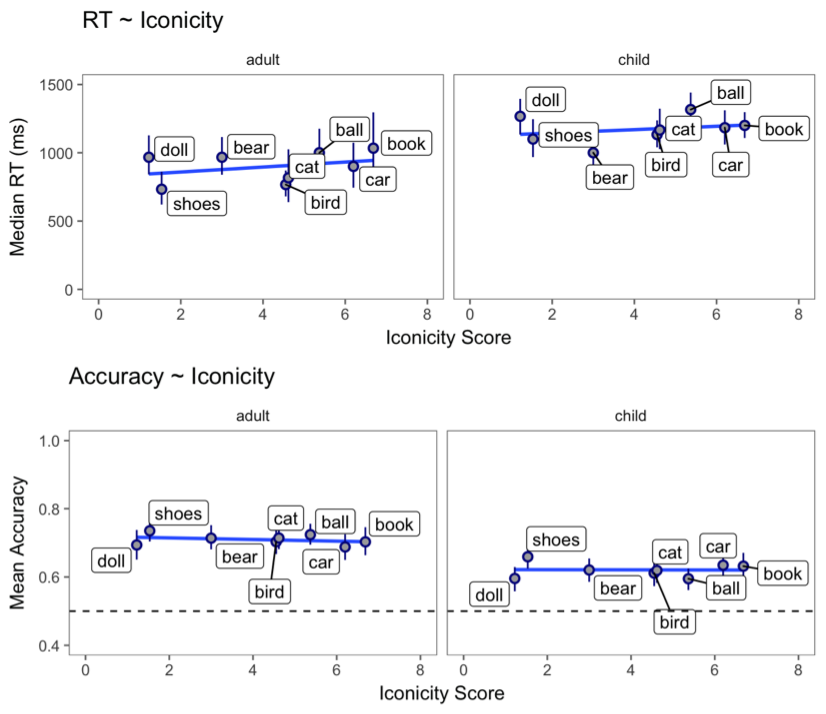
\includegraphics[width=0.75\linewidth]{/Users/ejyoon/Documents/Documents/Research/dissertation/index/chapter_child_rmds/SOL/figures/iconicity} 

}

\caption[Association between degree of iconicity and RT/Accuracy in Experiment 1.1]{Scatterplot of the association between degree of iconicity and RT (top row) and accuracy (bottom row) for both adults (left column) and children (right column). The blue line represents a linear model fit.}\label{fig:unnamed-chunk-12}
\end{figure}
Next, we performed a parallel analysis, exploring whether the iconicity
of our signs might have influenced adults and children's RT and
accuracy. It is possible that highly iconic signs might be easier to
process because of the visual similarity to the target object. Again, we
used ASL-LEX to quantify the iconicity of our signs. To generate these
values, native signers were asked to explicitly rate the iconicity of
each sign on a scale of 1-7, with 1 being not iconic at all and 7 being
very iconic. Similar to the phonological overlap analysis, we did see
evidence that degree of iconicity influenced either processing measure
for either age group in the VLP task.

\chapter{Supplementary materials for Chapter
3}\label{supplementary-materials-for-chapter-3}

\section{Model output for Experiment
3.1}\label{model-output-for-experiment-3.1}

\section{Model output for Experiment
3.2}\label{model-output-for-experiment-3.2}

\chapter{Supplementary materials for Chapter
4}\label{supplementary-materials-for-chapter-4}

\section{Analytic model specifications and
output}\label{analytic-model-specifications-and-output}

\subsection{Experiment 1}\label{experiment-1-1}

\captionsetup[table]{labelformat=empty}

\section*{Table A1. Length of inspection times on exposure trials in Experiment 1 as a function of gaze, interval, and number of referents}

\texttt{Log(Inspection time) $\sim$ (Gaze + Log(Interval) + Log(Referents))$^2$ + (1 | subject)}
\begin{table}[h]
\centering
\begin{tabular}{lrrrrl}
 term & estimate & std.error & t.value & p.value &  \\ 
  \hline
Intercept & 0.83 & 0.10 & 8.19 & $<$ .001 & *** \\ 
  Gaze Condition & 0.16 & 0.11 & 1.48 & 0.138 &  \\ 
  Log(Interval) & 0.06 & 0.05 & 1.33 & 0.184 &  \\ 
  Log(Referents) & 0.34 & 0.04 & 7.91 & $<$ .001 & *** \\ 
  Gaze Condition*Log(Interval) & -0.08 & 0.03 & -2.86 & 0.004 & ** \\ 
  Gaze Condition*Log(Referent) & -0.27 & 0.04 & -6.01 & $<$ .001 & *** \\ 
  Log(Interval)*Log(Referent) & -0.00 & 0.02 & -0.19 & 0.849 &  \\ 
   \hline
\end{tabular}
\label{tab:e1_rt}
\end{table}
\newpage

\section*{Table A2. Accuracy on test trials in Experiment 1 with inspection times on exposure trials included as a predictor}

\texttt{Correct $\sim$ (Trial Type + Gaze + Log(Interval) + Log(Referents) + \\ Log(Inspection Time))$^2$ + offset(logit($^1/_{Referents}$)) + (TrialType | subject)}
\begin{table}[h]
\centering
\begin{tabular}{lrrrrl}
 term & estimate & std.error & z.value & p.value &  \\ 
  \hline
Intercept & 2.89 & 0.34 & 8.49 & $<$ .001 & *** \\ 
  Switch Trial & -1.45 & 0.25 & -5.76 & $<$ .001 & *** \\ 
  Gaze Condition & 0.12 & 0.27 & 0.43 & 0.669 &  \\ 
  Log(Interval) & -0.47 & 0.11 & -4.15 & $<$ .001 & *** \\ 
  Log(Referents) & 0.05 & 0.14 & 0.39 & 0.693 &  \\ 
  Log(Inspection Time) & 0.20 & 0.15 & 1.38 & 0.169 &  \\ 
  Switch Trial*Gaze Condition & -1.02 & 0.13 & -7.86 & $<$ .001 & *** \\ 
  Switch Trial*Log(Interval) & 0.52 & 0.06 & 9.39 & $<$ .001 & *** \\ 
  Switch Trial*Log(Referent) & -0.62 & 0.09 & -6.67 & $<$ .001 & *** \\ 
  Switch Trial*Log(Inspection Time) & 0.09 & 0.07 & 1.36 & 0.174 &  \\ 
  Gaze Condition*Log(Interval) & 0.09 & 0.06 & 1.61 & 0.107 &  \\ 
  Gaze Condition*Log(Referent) & 0.36 & 0.10 & 3.68 & $<$ .001 & *** \\ 
  Gaze Condition*Log(Inspection Time) & -0.17 & 0.07 & -2.55 & 0.011 & * \\ 
  Log(Interval)*Log(Referent) & -0.05 & 0.04 & -1.26 & 0.207 &  \\ 
  Log(Interval)*Log(Inspection Time) & 0.02 & 0.03 & 0.54 & 0.589 &  \\ 
  Log(Referents)*Log(Inspection Time) & 0.05 & 0.05 & 0.94 & 0.345 &  \\ 
   \hline
\end{tabular}
\label{tab:e1_acc_it}
\end{table}
\newpage

\subsection{Experiment 2}\label{experiment-2-1}

\section*{Table A3. Length of inspection times on exposure trials in Experiment 2 as a function of gaze and interval}

\texttt{Log(Inspection time) $\sim$ Gaze * Log(Interval) + (1 | subject)}
\begin{table}[h]
\centering
\begin{tabular}{lrrrrl}
 term & estimate & std.error & t.value & p.value &  \\ 
  \hline
Intercept & 3.90 & 0.08 & 50.69 & $<$ .001 & *** \\ 
  Gaze Condition & -1.10 & 0.05 & -20.90 & $<$ .001 & *** \\ 
  Log(Interval) & -0.48 & 0.05 & -8.77 & $<$ .001 & *** \\ 
  Gaze Condition*Log(Interval) & -0.02 & 0.04 & -0.60 & 0.549 &  \\ 
   \hline
\end{tabular}
\label{tab:e2_rt}
\end{table}
\section*{Table A4. Accuracy on test trials in Experiment 2 with inspection times on exposure trials included as a predictor}

\texttt{Correct $\sim$ (Trial Type + Gaze + Log(Interval) + Log(Inspection Time))$^2$ + \\ offset(logit($^1/_{Referents}$)) + (TrialType | subject)}
\begin{table}[h]
\centering
\begin{tabular}{lrrrrl}
 term & estimate & std.error & z.value & p.value &  \\ 
  \hline
Intercept & 3.51 & 0.29 & 12.13 & $<$ .001 & *** \\ 
  Gaze Condition & 0.13 & 0.23 & 0.58 & 0.559 &  \\ 
  Switch Trial & -3.12 & 0.26 & -12.21 & $<$ .001 & *** \\ 
  Log(Interval) & -0.88 & 0.14 & -6.34 & $<$ .001 & *** \\ 
  Log(Inspection Time) & 0.15 & 0.13 & 1.14 & 0.255 &  \\ 
  Switch Trial*Gaze Condition & -0.54 & 0.17 & -3.21 & 0.001 & ** \\ 
  Gaze Condition*Log(Interval) & 0.16 & 0.09 & 1.85 & 0.064 & . \\ 
  Gaze Condition*Log(Inspection Time) & -0.14 & 0.10 & -1.37 & 0.172 &  \\ 
  Switch Trial*Log(Interval) & 0.77 & 0.10 & 8.00 & $<$ .001 & *** \\ 
  Switch Trial*Log(Inspection Time) & 0.21 & 0.11 & 1.96 & 0.05 & . \\ 
  Log(Interval)*Log(Inspection Time) & 0.04 & 0.06 & 0.77 & 0.44 &  \\ 
   \hline
\end{tabular}
\label{tab:e2_acc_it}
\end{table}
\newpage

\subsection{Experiment 3}\label{experiment-3-1}

\section*{Table A5. Accuracy on exposure trials in Experiment 3 as a function of reliability condition and participants' subjective reliability judgments}

\texttt{Correct-Exposure $\sim$ Reliability Condition * Subjective Reliability + \\  offset(logit($^1/_{Referents}$)) + (1 | subject)}
\begin{table}[h]
\centering
\begin{tabular}{lrrrrl}
 term & estimate & std.error & z.value & p.value &  \\ 
  \hline
Intercept & 3.07 & 0.98 & 3.13 & 0.002 & ** \\ 
  Reliability Condition & 3.28 & 1.50 & 2.19 & 0.029 & * \\ 
  Subjective Reliability & 7.26 & 1.73 & 4.21 & $<$ .001 & *** \\ 
  Reliability Condition*Subjective Reliability & -4.58 & 2.72 & -1.68 & 0.093 & . \\ 
   \hline
\end{tabular}
\label{tab:e3_gf_exp}
\end{table}
\section*{Table A6. Accuracy on test trials in Experiment 3 as a function of reliability condition}

\texttt{Correct $\sim$ Trial Type * Reliability Condition + offset(logit($^1/_{Referents}$)) + \\ (Trial Type | subject)}
\begin{table}[h]
\centering
\begin{tabular}{lrrrrl}
 term & estimate & std.error & z.value & p.value &  \\ 
  \hline
Intercept & 4.70 & 0.36 & 13.10 & $<$ .001 & *** \\ 
  Trial Type & -3.95 & 0.36 & -10.92 & $<$ .001 & *** \\ 
  Reliability Condition & 0.38 & 0.37 & 1.03 & 0.302 &  \\ 
  Reliability Condition*Trial Type & -0.76 & 0.38 & -2.01 & 0.044 & * \\ 
   \hline
\end{tabular}
\label{tab:e3_acc_rel_cond}
\end{table}
\newpage

\section*{Table A7. Accuracy on test trials in Experiment 3 as a function of reliability condition and participants' use of gaze on exposure trials}

\texttt{Correct $\sim$ (Trial Type + Reliability Condition + Correct-Exposure)$^2$ \\ + offset(logit($^1/_{Referents}$)) + (Trial Type | subject)}
\begin{table}[h]
\centering
\begin{tabular}{lrrrrl}
 term & estimate & std.error & z.value & p.value &  \\ 
  \hline
Intercept & 4.50 & 0.39 & 11.59 & $<$ .001 & *** \\ 
  Correct Exposure & 0.07 & 0.29 & 0.26 & 0.796 &  \\ 
  Trial Type & -2.70 & 0.38 & -7.07 & $<$ .001 & *** \\ 
  Reliability Condition & -0.43 & 0.44 & -0.98 & 0.325 &  \\ 
  Correct Exposure*Trial Type & -1.43 & 0.26 & -5.41 & $<$ .001 & *** \\ 
  Correct Exposure*Reliability & 0.97 & 0.33 & 2.92 & 0.004 & ** \\ 
  Reliability Condition*Trial Type & -0.62 & 0.36 & -1.72 & 0.086 & . \\ 
   \hline
\end{tabular}
\label{tab:e3_acc_rel_cond_gf}
\end{table}
\section*{Table A8. Accuracy on test trials in Experiment 3 as a function of each participants' accuracy on exposure trials}

\texttt{Correct $\sim$ Trial Type * Total Correct Exposure + offset(logit($^1/_{Referents}$)) + \\ (Trial Type | subject)}
\begin{table}[h]
\centering
\begin{tabular}{lrrrrl}
 term & estimate & std.error & z.value & p.value &  \\ 
  \hline
Intercept & 2.73 & 0.39 & 7.01 & $<$ .001 & *** \\ 
  Total Exposure Correct & 0.14 & 0.06 & 2.49 & 0.013 & * \\ 
  Trial Type & -1.39 & 0.39 & -3.55 & $<$ .001 & *** \\ 
  Total Exposure Correct*Trial Type & -0.26 & 0.06 & -4.66 & $<$ .001 & *** \\ 
   \hline
\end{tabular}
\label{tab:e3_acc_gaze_use}
\end{table}
\newpage

\section*{Table A9. Accuracy on test trials in Experiment 3 as a function of each participants' subjective reliability judgment}

\texttt{Correct $\sim$ Trial Type * Subjective Reliability + offset(logit($^1/_{Referents}$)) + \\ (Trial Type | subject)}
\begin{table}[h]
\centering
\begin{tabular}{lrrrrl}
 term & estimate & std.error & z.value & p.value &  \\ 
  \hline
Intercept & 4.54 & 0.44 & 10.33 & $<$ .001 & *** \\ 
  Subjective Reliability & 0.40 & 0.58 & 0.69 & 0.493 &  \\ 
  Trial Type & -3.44 & 0.44 & -7.81 & $<$ .001 & *** \\ 
  Subjective Reliability*Trial Type & -1.63 & 0.59 & -2.78 & 0.005 & ** \\ 
   \hline
\end{tabular}
\label{tab:e3_acc_subj_rel}
\end{table}
\section*{Table A10. Accuracy on test trials in Experiment 3 as a function of reliability condition and inspection time on exposure trials}

\texttt{Correct $\sim$ (Trial Type + Reliability condition + Trial Type + \\ Log(Inspection Time))$^2$ + offset(logit($^1/_{Referents}$)) + (Trial Type | subject)}
\begin{table}[h]
\centering
\begin{tabular}{lrrrrl}
 term & estimate & std.error & z.value & p.value &  \\ 
  \hline
Intercept & 3.11 & 0.20 & 15.94 & $<$ .001 & *** \\ 
  Log(Inspection Time) & 0.31 & 0.09 & 3.31 & 0.001 & ** \\ 
  Trial Type & -2.75 & 0.20 & -13.64 & $<$ .001 & *** \\ 
  Reliability Condition & 0.50 & 0.30 & 1.66 & 0.097 & . \\ 
  Log(Inspection Time)*Trial Type & 0.03 & 0.09 & 0.34 & 0.736 &  \\ 
  Log(Inspection Time)*Reliability Condition & -0.20 & 0.11 & -1.83 & 0.067 & . \\ 
  Trial Type*Reliability Condition & -0.58 & 0.29 & -1.97 & 0.048 & * \\ 
   \hline
\end{tabular}
\label{tab:e3_acc_inspect}
\end{table}
\newpage

\subsection{Experiment 4}\label{experiment-4-1}

\section*{Table A11. Accuracy on test trials in Experiment 4 as a function of gaze and interval}

\texttt{Correct $\sim$ (Trial Type + Gaze + Log(Interval))$^2$ + offset(logit($^1/_{Referents}$)) + \\ (Trial Type | subject)}
\begin{table}[h]
\centering
\begin{tabular}{lrrrrl}
 term & estimate & std.error & z.value & p.value &  \\ 
  \hline
Intercept & 3.37 & 0.16 & 21.32 & $<$ .001 & *** \\ 
  Trial Type & -3.18 & 0.16 & -19.93 & $<$ .001 & *** \\ 
  Gaze Condition & -0.48 & 0.14 & -3.52 & $<$ .001 & *** \\ 
  Log(Interval) & -0.84 & 0.10 & -8.59 & $<$ .001 & *** \\ 
  Trial Type*Gaze Condition & 0.90 & 0.14 & 6.63 & $<$ .001 & *** \\ 
  Trial Type*Log(Interval) & 0.80 & 0.09 & 8.71 & $<$ .001 & *** \\ 
  Gaze Condition*Log(Interval) & -0.01 & 0.07 & -0.10 & 0.917 &  \\ 
   \hline
\end{tabular}
\label{tab:e4_acc}
\end{table}
\chapter*{References}\label{references}
\addcontentsline{toc}{chapter}{References}

\markboth{References}{References}

\noindent

\setlength{\parindent}{-0.20in} \setlength{\leftskip}{0.20in}
\setlength{\parskip}{8pt}

\hypertarget{refs}{}
\hypertarget{ref-adriaans2017prosodic}{}
Adriaans, F., \& Swingley, D. (2017). Prosodic exaggeration within
infant-directed speech: Consequences for vowel learnability. \emph{The
Journal of the Acoustical Society of America}, \emph{141}(5),
3070--3078.

\hypertarget{ref-axia1985}{}
Axia, G., \& Baroni, M. R. (1985). Linguistic politeness at different
age levels. \emph{Child Development}, 918--927.

\hypertarget{ref-baldwin1993infants}{}
Baldwin, D. A. (1993). Infants' ability to consult the speaker for clues
to word reference. \emph{Journal of Child Language}, \emph{20}(02),
395--418.

\hypertarget{ref-baranes2015eye}{}
Baranes, A., Oudeyer, P.-Y., \& Gottlieb, J. (2015). Eye movements
reveal epistemic curiosity in human observers. \emph{Vision Research},
\emph{117}, 81--90.

\hypertarget{ref-barr2013random}{}
Barr, D. J., Levy, R., Scheepers, C., \& Tily, H. J. (2013). Random
effects structure for confirmatory hypothesis testing: Keep it maximal.
\emph{Journal of Memory and Language}, \emph{68}(3), 255--278.

\hypertarget{ref-bates2013lme4}{}
Bates, D., Maechler, M., Bolker, B., \& Walker, S. (2013). Lme4: Linear
mixed-effects models using eigen and s4. \emph{R Package Version},
\emph{1}(4).

\hypertarget{ref-begus2014infants}{}
Begus, K., Gliga, T., \& Southgate, V. (2014). Infants learn what they
want to learn: Responding to infant pointing leads to superior learning.

\hypertarget{ref-benitez2018predictable}{}
Benitez, V. L., \& Saffran, J. R. (2018). Predictable events enhance
word learning in toddlers. \emph{Current Biology}, \emph{28}(17),
2787--2793.

\hypertarget{ref-berlyne1960conflict}{}
Berlyne, D. E. (1960). Conflict, arousal, and curiosity.

\hypertarget{ref-birbili2009helping}{}
Birbili, M., \& Karagiorgou, I. (2009). Helping children and their
parents ask better questions: An intervention study. \emph{Journal of
Research in Childhood Education}, \emph{24}(1), 18--31.

\hypertarget{ref-bloom2002children}{}
Bloom, P. (2002). \emph{How children learn the meaning of words}. The
MIT Press.

\hypertarget{ref-bonawitz2016computational}{}
Bonawitz, E., \& Shafto, P. (2016). Computational models of development,
social influences. \emph{Current Opinion in Behavioral Sciences},
\emph{7}, 95--100.

\hypertarget{ref-bonawitz2011double}{}
Bonawitz, E., Shafto, P., Gweon, H., Goodman, N. D., Spelke, E., \&
Schulz, L. (2011). The double-edged sword of pedagogy: Instruction
limits spontaneous exploration and discovery. \emph{Cognition},
\emph{120}(3), 322--330.

\hypertarget{ref-bonnefon2009}{}
Bonnefon, J.-F., Feeney, A., \& Villejoubert, G. (2009). When some is
actually all: Scalar inferences in face-threatening contexts.
\emph{Cognition}, \emph{112}(2), 249--258.

\hypertarget{ref-boyd2011cultural}{}
Boyd, R., Richerson, P. J., \& Henrich, J. (2011). The cultural niche:
Why social learning is essential for human adaptation. \emph{Proceedings
of the National Academy of Sciences}, \emph{108}(Supplement 2),
10918--10925.

\hypertarget{ref-brooks2005development}{}
Brooks, R., \& Meltzoff, A. N. (2005). The development of gaze following
and its relation to language. \emph{Developmental Science}, \emph{8}(6),
535--543.

\hypertarget{ref-brooks2008infant}{}
Brooks, R., \& Meltzoff, A. N. (2008). Infant gaze following and
pointing predict accelerated vocabulary growth through two years of age:
A longitudinal, growth curve modeling study. \emph{Journal of Child
Language}, \emph{35}(01), 207--220.

\hypertarget{ref-brown1987}{}
Brown, P., \& Levinson, S. C. (1987). \emph{Politeness: Some universals
in language usage} (Vol. 4). Cambridge university press.

\hypertarget{ref-bruner1961act}{}
Bruner, J. S. (1961). The act of discovery. \emph{Harvard Educational
Review}.

\hypertarget{ref-butler2012preschoolers}{}
Butler, L. P., \& Markman, E. M. (2012). Preschoolers use intentional
and pedagogical cues to guide inductive inferences and exploration.
\emph{Child Development}, \emph{83}(4), 1416--1428.

\hypertarget{ref-call2005copying}{}
Call, J., Carpenter, M., \& Tomasello, M. (2005). Copying results and
copying actions in the process of social learning: Chimpanzees (pan
troglodytes) and human children (homo sapiens). \emph{Animal Cognition},
\emph{8}(3), 151--163.

\hypertarget{ref-carlson2001individual}{}
Carlson, S. M., \& Moses, L. J. (2001). Individual differences in
inhibitory control and children's theory of mind. \emph{Child
Development}, \emph{72}(4), 1032--1053.

\hypertarget{ref-carpenter1998social}{}
Carpenter, M., Nagell, K., Tomasello, M., Butterworth, G., \& Moore, C.
(1998). Social cognition, joint attention, and communicative competence
from 9 to 15 months of age. \emph{Monographs of the Society for Research
in Child Development}, i--174.

\hypertarget{ref-cartmill2013quality}{}
Cartmill, E. A., Armstrong, B. F., Gleitman, L. R., Goldin-Meadow, S.,
Medina, T. N., \& Trueswell, J. C. (2013). Quality of early parent input
predicts child vocabulary 3 years later. \emph{Proceedings of the
National Academy of Sciences}, \emph{110}(28), 11278--11283.

\hypertarget{ref-castro2009human}{}
Castro, R. M., Kalish, C., Nowak, R., Qian, R., Rogers, T., \& Zhu, X.
(2009). Human active learning. In \emph{Advances in neural information
processing systems} (pp. 241--248).

\hypertarget{ref-chi2009active}{}
Chi, M. T. (2009). Active-constructive-interactive: A conceptual
framework for differentiating learning activities. \emph{Topics in
Cognitive Science}, \emph{1}(1), 73--105.

\hypertarget{ref-chow2008see}{}
Chow, V., Poulin-Dubois, D., \& Lewis, J. (2008). To see or not to see:
Infants prefer to follow the gaze of a reliable looker.
\emph{Developmental Science}, \emph{11}(5), 761--770.

\hypertarget{ref-cimpian2007subtle}{}
Cimpian, A., Arce, H.-M. C., Markman, E. M., \& Dweck, C. S. (2007).
Subtle linguistic cues affect children's motivation. \emph{Psychological
Science}, \emph{18}(4), 314--316.

\hypertarget{ref-clark2009first}{}
Clark, E. V. (2009). \emph{First language acquisition}. Cambridge
University Press.

\hypertarget{ref-clark1980}{}
Clark, H. H., \& Schunk, D. H. (1980). Polite responses to polite
requests. \emph{Cognition}, \emph{8}(2), 111--143.

\hypertarget{ref-cleveland2007joint}{}
Cleveland, A., Schug, M., \& Striano, T. (2007). Joint attention and
object learning in 5-and 7-month-old infants. \emph{Infant and Child
Development}, \emph{16}(3), 295--306.

\hypertarget{ref-coenen2017asking}{}
Coenen, A., Nelson, J. D., \& Gureckis, T. (2017). Asking the right
questions about human inquiry.

\hypertarget{ref-colombo2001development}{}
Colombo, J. (2001). The development of visual attention in infancy.
\emph{Annual Review of Psychology}, \emph{52}(1), 337--367.

\hypertarget{ref-cook2011science}{}
Cook, C., Goodman, N. D., \& Schulz, L. E. (2011). Where science starts:
Spontaneous experiments in preschoolers' exploratory play.
\emph{Cognition}, \emph{120}(3), 341--349.

\hypertarget{ref-cooper1990preference}{}
Cooper, R. P., \& Aslin, R. N. (1990). Preference for infant-directed
speech in the first month after birth. \emph{Child Development},
\emph{61}(5), 1584--1595.

\hypertarget{ref-corriveau2009choosing}{}
Corriveau, K., \& Harris, P. L. (2009). Choosing your informant:
Weighing familiarity and recent accuracy. \emph{Developmental Science},
\emph{12}(3), 426--437.

\hypertarget{ref-cottrell1968social}{}
Cottrell, N. B., Wack, D. L., Sekerak, G. J., \& Rittle, R. H. (1968).
Social facilitation of dominant responses by the presence of an audience
and the mere presence of others. \emph{Journal of Personality and Social
Psychology}, \emph{9}(3), 245.

\hypertarget{ref-csibra2009natural}{}
Csibra, G., \& Gergely, G. (2009). Natural pedagogy. \emph{Trends in
Cognitive Sciences}, \emph{13}(4), 148--153.

\hypertarget{ref-de2003investigating}{}
De Boer, B., \& Kuhl, P. K. (2003). Investigating the role of
infant-directed speech with a computer model. \emph{Acoustics Research
Letters Online}, \emph{4}(4), 129--134.

\hypertarget{ref-deborah2004children}{}
Deborah, G. K. N., Louisa Chan, E., \& Holt, M. B. (2004). When children
ask,``What is it?'' what do they want to know about artifacts?
\emph{Psychological Science}, \emph{15}(6), 384--389.

\hypertarget{ref-decasper1987human}{}
DeCasper, A. J., Fifer, W. P., Oates, J., \& Sheldon, S. (1987). Of
human bonding: Newborns prefer their mothers' voices. \emph{Cognitive
Development in Infancy}, 111--118.

\hypertarget{ref-dweck1988social}{}
Dweck, C. S., \& Leggett, E. L. (1988). A social-cognitive approach to
motivation and personality. \emph{Psychological Review}, \emph{95}(2),
256.

\hypertarget{ref-eaves2016infant}{}
Eaves Jr, B. S., Feldman, N. H., Griffiths, T. L., \& Shafto, P. (2016).
Infant-directed speech is consistent with teaching. \emph{Psychological
Review}, \emph{123}(6), 758.

\hypertarget{ref-emery1998optimal}{}
Emery, A., \& Nenarokomov, A. V. (1998). Optimal experiment design.
\emph{Measurement Science and Technology}, \emph{9}(6), 864.

\hypertarget{ref-farroni2002eye}{}
Farroni, T., Csibra, G., Simion, F., \& Johnson, M. H. (2002). Eye
contact detection in humans from birth. \emph{Proceedings of the
National Academy of Sciences}, \emph{99}(14), 9602--9605.

\hypertarget{ref-farroni2007direct}{}
Farroni, T., Massaccesi, S., Menon, E., \& Johnson, M. H. (2007). Direct
gaze modulates face recognition in young infants. \emph{Cognition},
\emph{102}(3), 396--404.

\hypertarget{ref-fernald1987acoustic}{}
Fernald, A., \& Kuhl, P. (1987). Acoustic determinants of infant
preference for motherese speech. \emph{Infant Behavior and Development},
\emph{10}(3), 279--293.

\hypertarget{ref-fernald1991prosody}{}
Fernald, A., \& Mazzie, C. (1991). Prosody and focus in speech to
infants and adults. \emph{Developmental Psychology}, \emph{27}(2), 209.

\hypertarget{ref-fernald1998rapid}{}
Fernald, A., Pinto, J. P., Swingley, D., Weinbergy, A., \& McRoberts, G.
W. (1998). Rapid gains in speed of verbal processing by infants in the
2nd year. \emph{Psychological Science}, \emph{9}(3), 228--231.

\hypertarget{ref-fitneva2013development}{}
Fitneva, S. A., Lam, N. H., \& Dunfield, K. A. (2013). The development
of children's information gathering: To look or to ask?
\emph{Developmental Psychology}, \emph{49}(3), 533.

\hypertarget{ref-franchak2018see}{}
Franchak, J. M., Kretch, K. S., \& Adolph, K. E. (2018). See and be
seen: Infant--caregiver social looking during locomotor free play.
\emph{Developmental Science}, \emph{21}(4), e12626.

\hypertarget{ref-frank2012predicting}{}
Frank, M. C., \& Goodman, N. D. (2012). Predicting pragmatic reasoning
in language games. \emph{Science}, \emph{336}(6084), 998--998.

\hypertarget{ref-frank2014inferring}{}
Frank, M. C., \& Goodman, N. D. (2014). Inferring word meanings by
assuming that speakers are informative. \emph{Cognitive Psychology},
\emph{75}, 80--96.

\hypertarget{ref-frank2009using}{}
Frank, M. C., Goodman, N. D., \& Tenenbaum, J. B. (2009). Using
speakers' referential intentions to model early cross-situational word
learning. \emph{Psychological Science}, \emph{20}(5), 578--585.

\hypertarget{ref-frank2013social}{}
Frank, M. C., Tenenbaum, J. B., \& Fernald, A. (2013). Social and
discourse contributions to the determination of reference in
cross-situational word learning. \emph{Language Learning and
Development}, \emph{9}(1), 1--24.

\hypertarget{ref-frazier2009preschoolers}{}
Frazier, B. N., Gelman, S. A., \& Wellman, H. M. (2009). Preschoolers'
search for explanatory information within adult--child conversation.
\emph{Child Development}, \emph{80}(6), 1592--1611.

\hypertarget{ref-friesen2004attentional}{}
Friesen, C. K., Ristic, J., \& Kingstone, A. (2004). Attentional effects
of counterpredictive gaze and arrow cues. \emph{Journal of Experimental
Psychology: Human Perception and Performance}, \emph{30}(2), 319.

\hypertarget{ref-geisler2003ideal}{}
Geisler, W. S. (2003). Ideal observer analysis. \emph{The Visual
Neurosciences}, \emph{10}(7), 12--12.

\hypertarget{ref-gelman2009learning}{}
Gelman, S. A. (2009). Learning from others: Children's construction of
concepts. \emph{Annual Review of Psychology}, \emph{60}, 115--140.

\hypertarget{ref-gelman2008generic}{}
Gelman, S. A., Goetz, P. J., Sarnecka, B. W., \& Flukes, J. (2008).
Generic language in parent-child conversations. \emph{Language Learning
and Development}, \emph{4}(1), 1--31.

\hypertarget{ref-gergely2007pedagogy}{}
Gergely, G., Egyed, K., \& Király, I. (2007). On pedagogy.
\emph{Developmental Science}, \emph{10}(1), 139--146.

\hypertarget{ref-gerken2011infants}{}
Gerken, L., Balcomb, F. K., \& Minton, J. L. (2011). Infants avoid
`labouring in vain'by attending more to learnable than unlearnable
linguistic patterns. \emph{Developmental Science}, \emph{14}(5),
972--979.

\hypertarget{ref-gerstenberg2017intuitive}{}
Gerstenberg, T., \& Tenenbaum, J. B. (2017). Intuitive theories.
\emph{Oxford Handbook of Causal Reasoning}, 515--548.

\hypertarget{ref-gillette1999human}{}
Gillette, J., Gleitman, H., Gleitman, L., \& Lederer, A. (1999). Human
simulations of vocabulary learning. \emph{Cognition}, \emph{73}(2),
135--176.

\hypertarget{ref-gleitman1990structural}{}
Gleitman, L. (1990). The structural sources of verb meanings.
\emph{Language Acquisition}, \emph{1}(1), 3--55.

\hypertarget{ref-goffman1967}{}
Goffman, E. (1967). \emph{Interaction ritual: Essays on face-to-face
interaction}. Aldine.

\hypertarget{ref-goldstein2008social}{}
Goldstein, M. H., \& Schwade, J. A. (2008). Social feedback to infants'
babbling facilitates rapid phonological learning. \emph{Psychological
Science}, \emph{19}(5), 515--523.

\hypertarget{ref-goodman2016pragmatic}{}
Goodman, N. D., \& Frank, M. C. (2016). Pragmatic language
interpretation as probabilistic inference. \emph{Trends in Cognitive
Sciences}, \emph{20}(11), 818--829.

\hypertarget{ref-goodman2009cause}{}
Goodman, N. D., Baker, C. L., \& Tenenbaum, J. B. (2009). Cause and
intent: Social reasoning in causal learning. In \emph{Proceedings of the
31st annual conference of the cognitive science society} (pp.
2759--2764).

\hypertarget{ref-gopnik1999scientist}{}
Gopnik, A., Meltzoff, A. N., \& Kuhl, P. K. (1999). \emph{The scientist
in the crib: Minds, brains, and how children learn.} William Morrow \&
Co.

\hypertarget{ref-gottlieb2012attention}{}
Gottlieb, J. (2012). Attention, learning, and the value of information.
\emph{Neuron}, \emph{76}(2), 281--295.

\hypertarget{ref-gottlieb2018towards}{}
Gottlieb, J., \& Oudeyer, P.-Y. (2018). Towards a neuroscience of active
sampling and curiosity. \emph{Nature Reviews Neuroscience}, 1.

\hypertarget{ref-grabinger1995rich}{}
Grabinger, R. S., \& Dunlap, J. C. (1995). Rich environments for active
learning: A definition. \emph{Research in Learning Technology},
\emph{3}(2).

\hypertarget{ref-graf2013infant}{}
Graf Estes, K., \& Hurley, K. (2013). Infant-directed prosody helps
infants map sounds to meanings. \emph{Infancy}, \emph{18}(5), 797--824.

\hypertarget{ref-grice1975}{}
Grice, H. P. (1975). Logic and conversation. In P. Cole \& J. L. Morgan
(Eds.), \emph{Syntax and semantics} (Vol. 3, pp. 41--58). Academic
Press.

\hypertarget{ref-griffiths2015rational}{}
Griffiths, T. L., Lieder, F., \& Goodman, N. D. (2015). Rational use of
cognitive resources: Levels of analysis between the computational and
the algorithmic. \emph{Topics in Cognitive Science}, \emph{7}(2),
217--229.

\hypertarget{ref-gunderson2013parent}{}
Gunderson, E. A., Gripshover, S. J., Romero, C., Dweck, C. S.,
Goldin-Meadow, S., \& Levine, S. C. (2013). Parent praise to 1-to
3-year-olds predicts children's motivational frameworks 5 years later.
\emph{Child Development}, \emph{84}(5), 1526--1541.

\hypertarget{ref-gureckis2012self}{}
Gureckis, T. M., \& Markant, D. B. (2012). Self-directed learning a
cognitive and computational perspective. \emph{Perspectives on
Psychological Science}, \emph{7}(5), 464--481.

\hypertarget{ref-gweon201116}{}
Gweon, H., \& Schulz, L. (2011). 16-month-olds rationally infer causes
of failed actions. \emph{Science}, \emph{332}(6037), 1524--1524.

\hypertarget{ref-gweon2014sins}{}
Gweon, H., Pelton, H., Konopka, J. A., \& Schulz, L. E. (2014). Sins of
omission: Children selectively explore when teachers are
under-informative. \emph{Cognition}, \emph{132}(3), 335--341.

\hypertarget{ref-haertel2008return}{}
Haertel, R. A., Seppi, K. D., Ringger, E. K., \& Carroll, J. L. (2008).
Return on investment for active learning. In \emph{Proceedings of the
nips workshop on cost-sensitive learning} (Vol. 72).

\hypertarget{ref-hayhoe2005eye}{}
Hayhoe, M., \& Ballard, D. (2005). Eye movements in natural behavior.
\emph{Trends in Cognitive Sciences}, \emph{9}(4), 188--194.

\hypertarget{ref-henderson2007visual}{}
Henderson, J. M., Brockmole, J. R., Castelhano, M. S., \& Mack, M.
(2007). Visual saliency does not account for eye movements during visual
search in real-world scenes. In \emph{Eye movements} (pp. 537--III).
Elsevier.

\hypertarget{ref-hills2012optimal}{}
Hills, T. T., Jones, M. N., \& Todd, P. M. (2012). Optimal foraging in
semantic memory. \emph{Psychological Review}, \emph{119}(2), 431.

\hypertarget{ref-hollich2000breaking}{}
Hollich, G. J., Hirsh-Pasek, K., Golinkoff, R. M., Brand, R. J., Brown,
E., Chung, H. L., \ldots{} Bloom, L. (2000). Breaking the language
barrier: An emergentist coalition model for the origins of word
learning. \emph{Monographs of the Society for Research in Child
Development}, i--135.

\hypertarget{ref-holtgraves1997}{}
Holtgraves, T. (1997). YES, but... positive politeness in conversation
arguments. \emph{Journal of Language and Social Psychology},
\emph{16}(2), 222--239.

\hypertarget{ref-ide1989}{}
Ide, S. (1989). Formal forms and discernment: Two neglected aspects of
universals of linguistic politeness. \emph{Multilingua-Journal of
Cross-Cultural and Interlanguage Communication}, \emph{8}(2-3),
223--248.

\hypertarget{ref-jara2015children}{}
Jara-Ettinger, J., Gweon, H., Tenenbaum, J. B., \& Schulz, L. E. (2015).
Children's understanding of the costs and rewards underlying rational
action. \emph{Cognition}, \emph{140}, 14--23.

\hypertarget{ref-johnson1991newborns}{}
Johnson, M. H., Dziurawiec, S., Ellis, H., \& Morton, J. (1991).
Newborns' preferential tracking of face-like stimuli and its subsequent
decline. \emph{Cognition}, \emph{40}(1), 1--19.

\hypertarget{ref-kachergis2013actively}{}
Kachergis, G., Yu, C., \& Shiffrin, R. M. (2013). Actively learning
object names across ambiguous situations. \emph{Topics in Cognitive
Science}, \emph{5}(1), 200--213.

\hypertarget{ref-kanwisher1997locus}{}
Kanwisher, N., Woods, R. P., Iacoboni, M., \& Mazziotta, J. C. (1997). A
locus in human extrastriate cortex for visual shape analysis.
\emph{Journal of Cognitive Neuroscience}, \emph{9}(1), 133--142.

\hypertarget{ref-kidd2012goldilocks}{}
Kidd, C., Piantadosi, S. T., \& Aslin, R. N. (2012). The goldilocks
effect: Human infants allocate attention to visual sequences that are
neither too simple nor too complex. \emph{PloS One}, \emph{7}(5),
e36399.

\hypertarget{ref-kidd2014goldilocks}{}
Kidd, C., Piantadosi, S. T., \& Aslin, R. N. (2014). The goldilocks
effect in infant auditory attention. \emph{Child Development},
\emph{85}(5), 1795--1804.

\hypertarget{ref-kim2016young}{}
Kim, S., Paulus, M., Sodian, B., \& Proust, J. (2016). Young children's
sensitivity to their own ignorance in informing others. \emph{PloS One},
\emph{11}(3), e0152595.

\hypertarget{ref-klahr2004equivalence}{}
Klahr, D., \& Nigam, M. (2004). The equivalence of learning paths in
early science instruction effects of direct instruction and discovery
learning. \emph{Psychological Science}, \emph{15}(10), 661--667.

\hypertarget{ref-kline2015learn}{}
Kline, M. A. (2015). How to learn about teaching: An evolutionary
framework for the study of teaching behavior in humans and other
animals. \emph{Behavioral and Brain Sciences}, \emph{38}.

\hypertarget{ref-koehne2014interplay}{}
Koehne, J., \& Crocker, M. W. (2014). The interplay of cross-situational
word learning and sentence-level constraints. \emph{Cognitive Science}.

\hypertarget{ref-koenig2004trust}{}
Koenig, M. A., Clement, F., \& Harris, P. L. (2004). Trust in testimony:
Children's use of true and false statements. \emph{Psychological
Science}, \emph{15}(10), 694--698.

\hypertarget{ref-kontra2012embodied}{}
Kontra, C., Goldin-Meadow, S., \& Beilock, S. L. (2012). Embodied
learning across the life span. \emph{Topics in Cognitive Science},
\emph{4}(4), 731--739.

\hypertarget{ref-kuhl2007speech}{}
Kuhl, P. K. (2007). Is speech learning `gated'by the social brain?
\emph{Developmental Science}, \emph{10}(1), 110--120.

\hypertarget{ref-kuhn2008needs}{}
Kuhn, D., \& Pease, M. (2008). What needs to develop in the development
of inquiry skills? \emph{Cognition and Instruction}, \emph{26}(4),
512--559.

\hypertarget{ref-leech1983}{}
Leech, G. (1983). \emph{Principles of pragmatics}. London, New York:
Longman Group Ltd.

\hypertarget{ref-legare2013use}{}
Legare, C. H., Mills, C. M., Souza, A. L., Plummer, L. E., \& Yasskin,
R. (2013). The use of questions as problem-solving strategies during
early childhood. \emph{Journal of Experimental Child Psychology},
\emph{114}(1), 63--76.

\hypertarget{ref-lenth2016lsmeans}{}
Lenth, R. V. (2016). Least-squares means: The R package lsmeans.
\emph{Journal of Statistical Software}, \emph{69}(1), 1--33.
\url{http://doi.org/10.18637/jss.v069.i01}

\hypertarget{ref-lindley1956measure}{}
Lindley, D. V. (1956). On a measure of the information provided by an
experiment. \emph{The Annals of Mathematical Statistics}, 986--1005.

\hypertarget{ref-lockhart2016could}{}
Lockhart, K. L., Goddu, M. K., Smith, E. D., \& Keil, F. C. (2016). What
could you really learn on your own?: Understanding the epistemic
limitations of knowledge acquisition. \emph{Child Development},
\emph{87}(2), 477--493.

\hypertarget{ref-lombrozo2006structure}{}
Lombrozo, T. (2006). The structure and function of explanations.
\emph{Trends in Cognitive Sciences}, \emph{10}(10), 464--470.

\hypertarget{ref-lyons2010metacognitive}{}
Lyons, K. E., \& Ghetti, S. (2010). Metacognitive development in early
childhood: New questions about old assumptions. In \emph{Trends and
prospects in metacognition research} (pp. 259--278). Springer.

\hypertarget{ref-macdonald2017info}{}
MacDonald, K., Blonder, A., Marchman, V., Fernald, A., \& Frank, M. C.
(2017a). An information-seeking account of eye movements during spoken
and signed language comprehension. In \emph{Proceedings of the 39th
annual conference of the cognitive science society}.

\hypertarget{ref-macdonald2018real}{}
MacDonald, K., LaMarr, T., Corina, D., Marchman, V. A., \& Fernald, A.
(2018). Real-time lexical comprehension in young children learning
american sign language. \emph{Developmental Science}, e12672.

\hypertarget{ref-macdonald2018noise}{}
MacDonald, K., Marchman, V., Fernald, A., \& Frank, M. C. (2018). Adults
and preschoolers seek visual information to support language
comprehension in noisy environments. In \emph{Proceedings of the 40th
annual conference of the cognitive science society}.

\hypertarget{ref-macdonald2013my}{}
MacDonald, K., Schug, M., Chase, E., \& Barth, H. (2013). My people,
right or wrong? Minimal group membership disrupts preschoolers'
selective trust. \emph{Cognitive Development}, \emph{28}(3), 247--259.

\hypertarget{ref-macdonald2017social}{}
MacDonald, K., Yurovsky, D., \& Frank, M. C. (2017b). Social cues
modulate the representations underlying cross-situational learning.
\emph{Cognitive Psychology}, \emph{94}, 67--84.

\hypertarget{ref-mackay2003information}{}
MacKay, D. J. (2003). \emph{Information theory, inference and learning
algorithms}. Cambridge university press.

\hypertarget{ref-maddux2011dissociations}{}
Maddux, J.-M., \& Holland, P. C. (2011). Dissociations between medial
prefrontal cortical subregions in the modulation of learning and action.
\emph{Behavioral Neuroscience}, \emph{125}(3), 383.

\hypertarget{ref-manohar2013attention}{}
Manohar, S. G., \& Husain, M. (2013). Attention as foraging for
information and value. \emph{Frontiers in Human Neuroscience}, \emph{7},
711.

\hypertarget{ref-marchman2008speed}{}
Marchman, V. A., \& Fernald, A. (2008). Speed of word recognition and
vocabulary knowledge in infancy predict cognitive and language outcomes
in later childhood. \emph{Developmental Science}, \emph{11}(3), F9--F16.

\hypertarget{ref-markant2014better}{}
Markant, D. B., \& Gureckis, T. M. (2014). Is it better to select or to
receive? Learning via active and passive hypothesis testing.
\emph{Journal of Experimental Psychology: General}, \emph{143}(1), 94.

\hypertarget{ref-markant2016enhanced}{}
Markant, D. B., Ruggeri, A., Gureckis, T. M., \& Xu, F. (2016). Enhanced
memory as a common effect of active learning. \emph{Mind, Brain, and
Education}, \emph{10}(3), 142--152.

\hypertarget{ref-markant2014deconstructing}{}
Markant, D., DuBrow, S., Davachi, L., \& Gureckis, T. M. (2014).
Deconstructing the effect of self-directed study on episodic memory.
\emph{Memory \& Cognition}, \emph{42}(8), 1211--1224.

\hypertarget{ref-markman1979realizing}{}
Markman, E. M. (1979). Realizing that you don't understand: Elementary
school children's awareness of inconsistencies. \emph{Child
Development}, 643--655.

\hypertarget{ref-matsumoto1988}{}
Matsumoto, Y. (1988). Reexamination of the universality of face:
Politeness phenomena in japanese. \emph{Journal of Pragmatics},
\emph{12}(4), 403--426.

\hypertarget{ref-mccormack2016children}{}
McCormack, T., Bramley, N., Frosch, C., Patrick, F., \& Lagnado, D.
(2016). Children's use of interventions to learn causal structure.
\emph{Journal of Experimental Child Psychology}, \emph{141}, 1--22.

\hypertarget{ref-mcmurray2012word}{}
McMurray, B., Horst, J. S., \& Samuelson, L. K. (2012). Word learning
emerges from the interaction of online referent selection and slow
associative learning. \emph{Psychological Review}, \emph{119}(4), 831.

\hypertarget{ref-medina2011words}{}
Medina, T. N., Snedeker, J., Trueswell, J. C., \& Gleitman, L. R.
(2011). How words can and cannot be learned by observation.
\emph{Proceedings of the National Academy of Sciences}, \emph{108}(22),
9014--9019.

\hypertarget{ref-mills2012little}{}
Mills, C. M., Danovitch, J. H., Grant, M. G., \& Elashi, F. B. (2012).
Little pitchers use their big ears: Preschoolers solve problems by
listening to others ask questions. \emph{Child Development},
\emph{83}(2), 568--580.

\hypertarget{ref-mills2010preschoolers}{}
Mills, C. M., Legare, C. H., Bills, M., \& Mejias, C. (2010).
Preschoolers use questions as a tool to acquire knowledge from different
sources. \emph{Journal of Cognition and Development}, \emph{11}(4),
533--560.

\hypertarget{ref-mills2011determining}{}
Mills, C. M., Legare, C. H., Grant, M. G., \& Landrum, A. R. (2011).
Determining who to question, what to ask, and how much information to
ask for: The development of inquiry in young children. \emph{Journal of
Experimental Child Psychology}, \emph{110}(4), 539--560.

\hypertarget{ref-najemnik2005optimal}{}
Najemnik, J., \& Geisler, W. S. (2005). Optimal eye movement strategies
in visual search. \emph{Nature}, \emph{434}(7031), 387.

\hypertarget{ref-needham2002pick}{}
Needham, A., Barrett, T., \& Peterman, K. (2002). A pick-me-up for
infants' exploratory skills: Early simulated experiences reaching for
objects using ``sticky mittens'' enhances young infants' object
exploration skills. \emph{Infant Behavior and Development},
\emph{25}(3), 279--295.

\hypertarget{ref-nelson2005finding}{}
Nelson, J. D. (2005). Finding useful questions: On bayesian
diagnosticity, probability, impact, and information gain.
\emph{Psychological Review}, \emph{112}(4).

\hypertarget{ref-nelson2010experience}{}
Nelson, J. D., McKenzie, C. R., Cottrell, G. W., \& Sejnowski, T. J.
(2010). Experience matters: Information acquisition optimizes
probability gain. \emph{Psychological Science}, \emph{21}(7), 960--969.

\hypertarget{ref-oakes2011infant}{}
Oakes, L. M. (2011). \emph{Infant perception and cognition: Recent
advances, emerging theories, and future directions}. Oxford University
Press, USA.

\hypertarget{ref-opfer2004revisiting}{}
Opfer, J. E., \& Siegler, R. S. (2004). Revisiting preschoolers' living
things concept: A microgenetic analysis of conceptual change in basic
biology. \emph{Cognitive Psychology}, \emph{49}(4), 301--332.

\hypertarget{ref-oudeyer2016evolution}{}
Oudeyer, P.-Y., \& Smith, L. B. (2016). How evolution may work through
curiosity-driven developmental process. \emph{Topics in Cognitive
Science}, \emph{8}(2), 492--502.

\hypertarget{ref-ouyang2016practical}{}
Ouyang, L., Tessler, M. H., Ly, D., \& Goodman, N. (2016). Practical
optimal experiment design with probabilistic programs. \emph{arXiv
Preprint arXiv:1608.05046}.

\hypertarget{ref-partridge2015young}{}
Partridge, E., McGovern, M. G., Yung, A., \& Kidd, C. (2015). Young
children's self-directed information gathering on touchscreens. In
\emph{Proceedings of the 37th annual conference of the cognitive science
society, austin, tx. cognitive science society}.

\hypertarget{ref-pea1982origins}{}
Pea, R. D. (1982). Origins of verbal logic: Spontaneous denials by
two-and three-year olds. \emph{Journal of Child Language}, \emph{9}(3),
597--626.

\hypertarget{ref-pegg1992preference}{}
Pegg, J. E., Werker, J. F., \& McLeod, P. J. (1992). Preference for
infant-directed over adult-directed speech: Evidence from 7-week-old
infants. \emph{Infant Behavior and Development}, \emph{15}(3), 325--345.

\hypertarget{ref-piaget1952origins}{}
Piaget, J., \& Cook, M. T. (1952). The origins of intelligence in
children.

\hypertarget{ref-pirolli1999information}{}
Pirolli, P., \& Card, S. (1999). Information foraging.
\emph{Psychological Review}, \emph{106}(4), 643.

\hypertarget{ref-prince2004does}{}
Prince, M. (2004). Does active learning work? A review of the research.
\emph{Journal of Engineering Education}, \emph{93}(3), 223--231.

\hypertarget{ref-quine19600}{}
Quine, W. V. (1960). 0. word and object. \emph{111e MIT Press}.

\hypertarget{ref-rakoczy2010bigger}{}
Rakoczy, H., Hamann, K., Warneken, F., \& Tomasello, M. (2010). Bigger
knows better: Young children selectively learn rule games from adults
rather than from peers. \emph{British Journal of Developmental
Psychology}, \emph{28}(4), 785--798.

\hypertarget{ref-ramirez2017active}{}
Ramirez-Loaiza, M. E., Sharma, M., Kumar, G., \& Bilgic, M. (2017).
Active learning: An empirical study of common baselines. \emph{Data
Mining and Knowledge Discovery}, \emph{31}(2), 287--313.

\hypertarget{ref-ratcliff2008diffusion}{}
Ratcliff, R., \& McKoon, G. (2008). The diffusion decision model: Theory
and data for two-choice decision tasks. \emph{Neural Computation},
\emph{20}(4), 873--922.

\hypertarget{ref-reid2005adult}{}
Reid, V. M., \& Striano, T. (2005). Adult gaze influences infant
attention and object processing: Implications for cognitive
neuroscience. \emph{European Journal of Neuroscience}, \emph{21}(6),
1763--1766.

\hypertarget{ref-rogoff1993guided}{}
Rogoff, B., Mistry, J., Göncü, A., Mosier, C., Chavajay, P., \& Heath,
S. B. (1993). Guided participation in cultural activity by toddlers and
caregivers. \emph{Monographs of the Society for Research in Child
Development}, i--179.

\hypertarget{ref-rohde2014markers}{}
Rohde, H., \& Frank, M. C. (2014). Markers of topical discourse in
child-directed speech. \emph{Cognitive Science}, \emph{38}(8),
1634--1661.

\hypertarget{ref-ross2003development}{}
Ross-sheehy, S., Oakes, L. M., \& Luck, S. J. (2003). The development of
visual short-term memory capacity in infants. \emph{Child Development},
\emph{74}(6), 1807--1822.

\hypertarget{ref-rothe2015asking}{}
Rothe, A., Lake, B. M., \& Gureckis, T. M. (2015). Asking useful
questions: Active learning with rich queries. In \emph{CogSci}.

\hypertarget{ref-rowe2017going}{}
Rowe, M. L., Leech, K. A., \& Cabrera, N. (2017). Going beyond input
quantity: Wh-questions matter for toddlers' language and cognitive
development. \emph{Cognitive Science}, \emph{41}(S1), 162--179.

\hypertarget{ref-ruggeri2015children}{}
Ruggeri, A., \& Lombrozo, T. (2015). Children adapt their questions to
achieve efficient search. \emph{Cognition}, \emph{143}, 203--216.

\hypertarget{ref-ruggeri2016active}{}
Ruggeri, A., Markant, D. B., Gureckis, T. M., \& Xu, F. (2016). Active
control of study leads to improved recognition memory in children. In
\emph{Proceedings of the 38th annual conference of the cognitive science
society. austin, tx: Cognitive science society}.

\hypertarget{ref-sage2011disentangling}{}
Sage, K. D., \& Baldwin, D. (2011). Disentangling the social and the
pedagogical in infants' learning about tool-use. \emph{Social
Development}, \emph{20}(4), 825--844.

\hypertarget{ref-schober1989understanding}{}
Schober, M. F., \& Clark, H. H. (1989). Understanding by addressees and
overhearers. \emph{Cognitive Psychology}, \emph{21}(2), 211--232.

\hypertarget{ref-schulz2012origins}{}
Schulz, L. (2012). The origins of inquiry: Inductive inference and
exploration in early childhood. \emph{Trends in Cognitive Sciences},
\emph{16}(7), 382--389.

\hypertarget{ref-senju2008gaze}{}
Senju, A., \& Csibra, G. (2008). Gaze following in human infants depends
on communicative signals. \emph{Current Biology}, \emph{18}(9),
668--671.

\hypertarget{ref-settles2012active}{}
Settles, B. (2012). Active learning. \emph{Synthesis Lectures on
Artificial Intelligence and Machine Learning}, \emph{6}(1), 1--114.

\hypertarget{ref-settles2008active}{}
Settles, B., Craven, M., \& Friedland, L. (2008). Active learning with
real annotation costs. In \emph{Proceedings of the nips workshop on
cost-sensitive learning} (pp. 1--10).

\hypertarget{ref-shafto2012epistemic}{}
Shafto, P., Eaves, B., Navarro, D. J., \& Perfors, A. (2012a). Epistemic
trust: Modeling children's reasoning about others' knowledge and intent.
\emph{Developmental Science}, \emph{15}(3), 436--447.

\hypertarget{ref-shafto2012learning}{}
Shafto, P., Goodman, N. D., \& Frank, M. C. (2012b). Learning from
others the consequences of psychological reasoning for human learning.
\emph{Perspectives on Psychological Science}, \emph{7}(4), 341--351.

\hypertarget{ref-shafto2014rational}{}
Shafto, P., Goodman, N. D., \& Griffiths, T. L. (2014). A rational
account of pedagogical reasoning: Teaching by, and learning from,
examples. \emph{Cognitive Psychology}, \emph{71}, 55--89.

\hypertarget{ref-singh2009influences}{}
Singh, L., Nestor, S., Parikh, C., \& Yull, A. (2009). Influences of
infant-directed speech on early word recognition. \emph{Infancy},
\emph{14}(6), 654--666.

\hypertarget{ref-siskind1996computational}{}
Siskind, J. M. (1996). A computational study of cross-situational
techniques for learning word-to-meaning mappings. \emph{Cognition},
\emph{61}(1), 39--91.

\hypertarget{ref-smith2011cross}{}
Smith, K., Smith, A. D., \& Blythe, R. A. (2011). Cross-situational
learning: An experimental study of word-learning mechanisms.
\emph{Cognitive Science}, \emph{35}(3), 480--498.

\hypertarget{ref-smith2008infants}{}
Smith, L. B., \& Yu, C. (2008). Infants rapidly learn word-referent
mappings via cross-situational statistics. \emph{Cognition},
\emph{106}(3), 1558--1568.

\hypertarget{ref-smith2013visual}{}
Smith, L. B., \& Yu, C. (2013). Visual attention is not enough:
Individual differences in statistical word-referent learning in infants.
\emph{Language Learning and Development}, \emph{9}(1), 25--49.

\hypertarget{ref-smith2014unrealized}{}
Smith, L. B., Suanda, S. H., \& Yu, C. (2014). The unrealized promise of
infant statistical word--referent learning. \emph{Trends in Cognitive
Sciences}, \emph{18}(5), 251--258.

\hypertarget{ref-stahl2015observing}{}
Stahl, A. E., \& Feigenson, L. (2015). Observing the unexpected enhances
infants' learning and exploration. \emph{Science}, \emph{348}(6230),
91--94.

\hypertarget{ref-tanenhaus2000eye}{}
Tanenhaus, M. K., Magnuson, J. S., Dahan, D., \& Chambers, C. (2000).
Eye movements and lexical access in spoken-language comprehension:
Evaluating a linking hypothesis between fixations and linguistic
processing. \emph{Journal of Psycholinguistic Research}, \emph{29}(6),
557--580.

\hypertarget{ref-thiessen2005infant}{}
Thiessen, E. D., Hill, E. A., \& Saffran, J. R. (2005). Infant-directed
speech facilitates word segmentation. \emph{Infancy}, \emph{7}(1),
53--71.

\hypertarget{ref-tomasello1986joint}{}
Tomasello, M., \& Farrar, M. J. (1986). Joint attention and early
language. \emph{Child Development}, 1454--1463.

\hypertarget{ref-trueswell2016perceiving}{}
Trueswell, J. C., Lin, Y., Armstrong, B., Cartmill, E. A.,
Goldin-Meadow, S., \& Gleitman, L. R. (2016). Perceiving referential
intent: Dynamics of reference in natural parent--child interactions.
\emph{Cognition}, \emph{148}, 117--135.

\hypertarget{ref-trueswell2013propose}{}
Trueswell, J. C., Medina, T. N., Hafri, A., \& Gleitman, L. (2013).
Propose but verify: Fast mapping meets cross-situational word learning.
\emph{Cognitive Psychology}, \emph{66}(1), 126--156.

\hypertarget{ref-uziel2007individual}{}
Uziel, L. (2007). Individual differences in the social facilitation
effect: A review and meta-analysis. \emph{Journal of Research in
Personality}, \emph{41}(3), 579--601.

\hypertarget{ref-vlach2013memory}{}
Vlach, H. A., \& Johnson, S. P. (2013). Memory constraints on infants'
cross-situational statistical learning. \emph{Cognition}, \emph{127}(3),
375--382.

\hypertarget{ref-vosniadou1992mental}{}
Vosniadou, S., \& Brewer, W. F. (1992). Mental models of the earth: A
study of conceptual change in childhood. \emph{Cognitive Psychology},
\emph{24}(4), 535--585.

\hypertarget{ref-vouloumanos2008fine}{}
Vouloumanos, A. (2008). Fine-grained sensitivity to statistical
information in adult word learning. \emph{Cognition}, \emph{107}(2),
729--742.

\hypertarget{ref-vouloumanos2007listening}{}
Vouloumanos, A., \& Werker, J. F. (2007). Listening to language at
birth: Evidence for a bias for speech in neonates. \emph{Developmental
Science}, \emph{10}(2), 159--164.

\hypertarget{ref-vredenburgh2016young}{}
Vredenburgh, C., \& Kushnir, T. (2016). Young children's help-seeking as
active information gathering. \emph{Cognitive Science}, \emph{40}(3),
697--722.

\hypertarget{ref-vul2014}{}
Vul, E., Goodman, N., Griffiths, T. L., \& Tenenbaum, J. B. (2014). One
and done? Optimal decisions from very few samples. \emph{Cognitive
Science}, \emph{38}(4), 599--637.

\hypertarget{ref-vygotsky1987zone}{}
Vygotsky, L. (1987). Zone of proximal development. \emph{Mind in
Society: The Development of Higher Psychological Processes},
\emph{5291}, 157.

\hypertarget{ref-watts2003}{}
Watts, R. J. (2003). \emph{Politeness}. Cambridge University Press.

\hypertarget{ref-woodard2016two}{}
Woodard, K., Gleitman, L. R., \& Trueswell, J. C. (2016). Two-and
three-year-olds track a single meaning during word learning: Evidence
for propose-but-verify. \emph{Language Learning and Development},
\emph{12}(3), 252--261.

\hypertarget{ref-wu2010no}{}
Wu, R., \& Kirkham, N. Z. (2010). No two cues are alike: Depth of
learning during infancy is dependent on what orients attention.
\emph{Journal of Experimental Child Psychology}, \emph{107}(2),
118--136.

\hypertarget{ref-wu2011infants}{}
Wu, R., Gopnik, A., Richardson, D. C., \& Kirkham, N. Z. (2011). Infants
learn about objects from statistics and people. \emph{Developmental
Psychology}, \emph{47}(5), 1220.

\hypertarget{ref-wu2015caregivers}{}
Wu, Z., \& Gros-Louis, J. (2015). Caregivers provide more labeling
responses to infants' pointing than to infants' object-directed
vocalizations. \emph{Journal of Child Language}, \emph{42}(3), 538--561.

\hypertarget{ref-xu2007sampling}{}
Xu, F., \& Tenenbaum, J. B. (2007a). Sensitivity to sampling in bayesian
word learning. \emph{Developmental Science}, \emph{10}(3), 288--297.

\hypertarget{ref-xu2007word}{}
Xu, F., \& Tenenbaum, J. B. (2007b). Word learning as bayesian
inference. \emph{Psychological Review}, \emph{114}(2), 245.

\hypertarget{ref-yoon2018balancing}{}
Yoon, E. J., MacDonald, K., Asaba, M., Gweon, H., \& Frank, M. C.
(2018). Balancing informational and social goals in active learning. In
\emph{Proceedings of the 40th annual conference of the cognitive science
society}.

\hypertarget{ref-yoonwon}{}
Yoon, E. J., Tessler, Michael Henry, Goodman, N. D., \& Frank, M. C.
(2017). ``I won't lie, it wasn't amazing'': Modeling polite indirect
speech. In \emph{Proceedings of the 39th annual conference of the
cognitive science society}.

\hypertarget{ref-yoon2008communication}{}
Yoon, J. M., Johnson, M. H., \& Csibra, G. (2008). Communication-induced
memory biases in preverbal infants. \emph{Proceedings of the National
Academy of Sciences}, \emph{105}(36), 13690--13695.

\hypertarget{ref-yu2007unified}{}
Yu, C., \& Ballard, D. H. (2007). A unified model of early word
learning: Integrating statistical and social cues.
\emph{Neurocomputing}, \emph{70}(13), 2149--2165.

\hypertarget{ref-yu2007rapid}{}
Yu, C., \& Smith, L. B. (2007). Rapid word learning under uncertainty
via cross-situational statistics. \emph{Psychological Science},
\emph{18}(5), 414--420.

\hypertarget{ref-yu2012embodied}{}
Yu, C., \& Smith, L. B. (2012). Embodied attention and word learning by
toddlers. \emph{Cognition}.

\hypertarget{ref-yu2013joint}{}
Yu, C., \& Smith, L. B. (2013). Joint attention without gaze following:
Human infants and their parents coordinate visual attention to objects
through eye-hand coordination. \emph{PloS One}, \emph{8}(11), e79659.

\hypertarget{ref-yu2016social}{}
Yu, C., \& Smith, L. B. (2016). The social origins of sustained
attention in one-year-old human infants. \emph{Current Biology},
\emph{26}(9), 1235--1240.

\hypertarget{ref-yu2005role}{}
Yu, C., Ballard, D. H., \& Aslin, R. N. (2005). The role of embodied
intention in early lexical acquisition. \emph{Cognitive Science},
\emph{29}(6), 961--1005.

\hypertarget{ref-yurovsky2014algorithmic}{}
Yurovsky, D., \& Frank, M. C. (2015). An integrative account of
constraints on cross-situational learning. \emph{Cognition}.

\hypertarget{ref-yurovsky2013statistical}{}
Yurovsky, D., Smith, L. B., \& Yu, C. (2013). Statistical word learning
at scale: The baby's view is better. \emph{Developmental Science},
\emph{16}(6), 959--966.

\hypertarget{ref-zangl2007increasing}{}
Zangl, R., \& Fernald, A. (2007). Increasing flexibility in children's
online processing of grammatical and nonce determiners in fluent speech.
\emph{Language Learning and Development}, \emph{3}(3), 199--231.


% Index?

\end{document}
